\chapter{Повышение интерпретируемости тематических моделей при помощи регуляризации}

В этом разделе будет предложен метод подбора коэффициентов сглаживания, коэффициентов разреживания и весов дополнительных модальностей. Также будет рассмотрен псевдорегуляризатор, основанный на допущении о функциональной зависимости $\Theta = f(\Phi)$ и превносящий в тематическую модель некоторые полезные свойства.

В данной главе ставится цель проанализировать поведение предложенного алгоритма на реальных текстовых коллекциях.

\section{Относительные коэффициенты регуляризации}

% Задача этого текста --- обьяснить теоретическую подоплёку относительных коэффициентов регуляризации и дать ряд практических советов по их применению.

% В данный момент открытая библиотека bigARTM умеет работать с относительными коэффициентами для $\phi$-регуляризаторов. Таким же образом можно подбирать и коэффициенты для $\theta$-регуляризаторов (возможность, которая сейчас в bigARTM отсутствует). Более того, таким же образом можно и подбирать веса дополнительных модальностей (возможность, которая и не снилась нашим мудрецам).

Относительные коэффициенты регуляризации были впервые введены в работе \cite{doykov} в общем виде.

\dscl{Общая формула взята из ВКР Никиты Дойкова. Важные частные случаи --- выведены мной, успешно проверены на практике}
В исследовании \cite{doykov} приведена формула для общего случая $k$ произвольных гладких регуляризаторов $R_i(\Phi, \Theta)$. Здесь и далее: $\tau_i$ (тау) обозначает абсолютный коэффициент регуляризации, а $\lambda_i$ - относительный коэффициент регуляризации

Общая формула для регуляризаторов $\Phi$:
\[
\phi_{wt} = \norm_{w \in W}\Bigg( 
    n_{wt} + \sum_{i=1}^k \lambda_i \Big[
        \gamma_i \frac{n_t}{r_{it}} + (1-\gamma_i)\frac{n}{r_i}
        \Big] 
    \phi_{wt} \frac{\partial R_i}{\partial \phi_{wt}}
\Bigg), \label{rel_phi_general}
\]

где: 
\begin{itemize}
    \item{$r_{it} = \sum_{w\in W} \Big| \phi_{wt} \frac{\partial R_i}{\partial \phi_{wt}} \Big| $ --- воздействие регуляризатора на тему}
    \item { $r_{i} = \sum_{t\in T} r_{it}$ --- суммарное воздействие регуляризатора на коллекцию.}
    \item { $\lambda_i$ - относительный коэффициент регуляризации, показывающий, \emph{во сколько раз} соответствующий регуляризатор влияет на оценку $\phi_{wt}$ больше, чем коллекция}
    \item {Выражение в квадратных скобках - \textit{фактор балансировки}, гарантирующий ''равновесие'' между $n_{wt}$ и регуляризационной добавкой}
\end{itemize}

Введённый в этой формуле коэффициент $\gamma_i$ отвечает за степень индивидуализации. Он позволяет плавно переходить от равномерной регуляризации по всем темам ($\gamma = 0$) к индивидуальному подходу к каждой теме ($\gamma = 1$).

Важно заметить следующие особенности: 
\begin{enumerate}
    \item {В формуле участвуют $n_t, r_{it}, r_{i}$:  величины, которые могут изменяться в ходе итераций EM-алгоритма. Следовательно, в общем случае
    абсолютные коэффициенты и относительные  коэффициенты задают различные множества возможных траекторий регуляризации.}
    \item  {В формуле участвуют $n_t, r_{it}, r_{i}$: переменные, значения которых определяются в ходе ЕМ-алгоритма.}
\end{enumerate}

Общая формула для регуляризаторов $\Theta$:

\[
\theta_{td} = \norm_{t \in T} \Bigg( 
    n_{td} + \sum_{i=1}^k \lambda_i \Big[
        \gamma_i \frac{n_d}{r_{id}} + (1-\gamma_i)\frac{n}{r_i}
        \Big] 
    \theta_{td} \frac{\partial R_i}{\partial \theta_{td}}
\Bigg), \label{rel_theta_general}
\]

где: 
\begin{itemize}
    \item { $r_{id} = \sum_{t\in T} \Big | \theta_{td} \frac{\partial R_i}{\partial \theta_{td}} \Big | $ --- воздействие регуляризатора на документ}
    \item { $r_{i} = \sum_{d\in D} r_{id}$ --- суммарное воздействие регуляризатора на коллекцию.}
    \item { $\lambda_i$ - относительный коэффициент регуляризации, показывающий, \emph{во сколько раз} соответствующий регуляризатор влияет на оценку $\theta_{td}$ больше, чем коллекция}
    \item {Выражение в квадратных скобках - \textit{фактор балансировки}, гарантирующий ''равновесие'' между $n_{td}$ и регуляризационной добавкой}
\end{itemize}

Вычисления по формуле \ref{rel_theta_general} являются проблематичными для онлайнового и пакетных ЕМ-алгоритмов. Это связано с тем, что алгоритм разбивает коллекцию документов на пакеты, обрабатываемые параллельно и связанные только посредством матрицы $\Phi$. Поскольку в общем случае вычисление $r_i$ требует информацию о всех документах сразу, то формула \ref{rel_theta_general} несовместима с архитектурой эффективного ЕМ-алгоритма.

Тем не менее, для ряда важных частных случаев подобрать относительные коэффициенты регуляризации всё-таки возможно.

\subsection{Важные частные случаи}
\dscl{Здесь есть неотвеченный вопрос: как в БигАРТМ работает относительная декорреляция. Фактор балансировки там скачет от итерации к итерации, мне кажется что этот вопрос стоит доисследовать}

\textbf{Утверждение}. Для регуляризаторов сглаживания и разреживания, каждый абсолютный коэффициент регуляризации математически равносилен некоторому относительному коэффиценту и наоборот.

\textbf{Сглаживание и разреживание Фи}. Формула M-шага, сглаживающего ($\tau > 0$) или разреживающего ($\tau < 0$) распределение $\phi_{wt}$:

\[
\phi_{wt} = \norm_{w \in W} \big( n_{wt} + \tau \big)
\]

Интуитивный смысл этого преобразования прост: мы либо ''притягиваем'' Фи к равномерному распределению $\beta = \frac{1}{|W|}$, либо ''отталкиваем'' её от него же (возможно, даже зануляя при этом какие-то компоненты).

Оказывается, можно провести репараметризацию, которая строго это продемонстрирует. 

Пусть $\beta = \frac{1}{|W|}$ --- равномерное распределение, а текущие значения $n_{wt}$ и $\tau \in \mathbb{R}$ таковы, что на этой итерации M-шага зануления компонент не происходит (то есть либо $\tau > 0$, либо $\tau < 0$, но $n_{wt} + \tau > 0$).

Тогда операцию положительной обрезки можно проигнорировать:

\[
\phi_{wt} = \norm_{w \in W} \big( n_{wt} + \tau \big) = \frac{n_{wt} + \tau }{\sum_{w \in W} n_{wt} + \tau } = \frac{n_{wt} + \tau }{n_{t} + \tau |W|}  
\]

Попробуем представить это выражение, как выпуклую комбинацию распределений  $\frac{n_{wt}}{n_t}$ (оценки максимума правдоподобия) и $\frac{1}{|W|}$ (равномерного распределения). 


\[
\frac{n_{wt} + \tau}{n_{t} + \tau |W|} = (1-\lambda) \frac{n_{wt}}{n_t} + \lambda \frac{1}{|W|} \iff \tau  = \frac{n_t \lambda}{(1-\lambda) |W|} \label{sp_phi_rel2abs} 
\]

Значит, сглаживание Фи можно трактовать, как нахождение компромисса между $\phi_{wt} = \frac{n_{wt}}{n_t}$ и $\phi_{wt} = \frac{1}{|W|}$. 

Что это означает на практике? Допустим, мы хотим провести регуляризацию так, чтобы $\phi_{wt}$ на 50\% состояла из оценки максимума правдоподобия, и на 50\% из априорного распределения $\frac{1}{|W|}$. Для этого достаточно вычислить $\tau$ по формуле и подставить в модель.

Важно заметить следующие особенности: 

\begin{enumerate}
    \item  {Полученный коэффициент регуляризации зависит от $n_t$, то есть разные темы будут сглаживаться/разреживаться с разной силой}
    \item  {Поскольку значение $n_t$ может изменяться в ходе итераций EM-алгоритма, то абсолютная величина коэффициента тоже может меняется со временем}
    \item  {Зависит от $|W|$. Это значит, что один и тот же абсолютный коэффициент сглаживания/разреживания может по-разному влиять на коллекцию в зависимости от размера словаря.  Формула \ref{sp_phi_rel2abs} делает эту зависимость более наглядной. Теперь можно эвристически прикинуть, как нужно пересчитать $\tau$ при изменении словаря (например, после выкидывания слишком редких или частых слов).}
\end{enumerate}

Особенность (1) добавляет гибкости, но может быть проблематична на практике (слишком много дополнительных степеней свободы, возможен оверфиттинг).

В работе \cite{doykov} было предложено усреднить по всем темам:

\[
\tau = \frac{1}{|T|} \sum_t \tau_t = \frac{n}{|T|\cdot|W|} \frac{\lambda}{(1-\lambda)}
\]

\textbf{Сглаживание и разреживание Теты}. Вспомним, что M-шаг для Теты выглядит таким образом:

\[
\theta_{td} = \norm_{t \in T} \big( n_{td} + \tau \big)
\]

Аналогично выведем формулу:

\[
\frac{n_{td} + \tau}{n_d + \tau |T|} = (1-\lambda) \frac{n_{td}}{n_d} + \lambda \frac{1}{|T|} \iff \tau = \frac{n_d \lambda}{(1-\lambda) |T|} \label{sp_theta_rel2abs} 
\]

Полученный коэффициент регуляризации зависит от $n_d$, то есть разные документы будут сглаживаться/разреживаться с разной силой. Можно также усреднить все $\tau$ по документам:

\[
\tau = \frac{\lambda \sum_d n_d }{(1-\lambda) |D| \cdot |T|} 
\]

Заметим, что обе формулы для $\tau$ \textit{стабильны}. В отличии от $n_t$, значение $n_d$ в ходе обучения \emph{не меняется}. Все использованные здесь величины заранее известны и постоянны.

Следовательно, если рассматривать лишь усреднённые коэффиценты, то каждый относительный коэффициент регуляризации математически равносилен некоторому абсолютному коэффиценту и наоборот.

\textbf{Многомодальное тематическое моделирование}


Вспомним, что вероятность появления термина $w$ из $k$-й модальности в документе $d$ задаётся следующей формулой:
$p(w^k \cond d) = \sum_t \phi_{wt}^k \theta_{td}$, а общее правдоподобие представляется так:

\[
L(\Phi^m, \Theta) = \sum_m \tau_m \sum_{d\in D} \sum_{w \in W^m} n_{dw} \ln p(w \cond d) \rightarrow \max, \label{modal_likelihood}
\]
где коэффиценты $\tau_m$ показывают \textit{вес} модальности $m$.

Известно, что $EM$-алгоритм для мультимодальной тематической модели структурно похож на классический $EM$-алгоритм \cite{yanina}\cite{vorontsov2015non}\cite{bulatov}. 

Формулу \ref{modal_likelihood} можно проинтерпретировать, как введение $M-1$ дополнительного регуляризатора с коэффициентами $\tau_m$ \cite{yanina}:

\[
\tau_m R(\Phi, \Theta)_m = \tau_m L^{(m)}(\Phi, \Theta) = \tau_m  \sum_d \sum_w n_{dw}^{(m)} \ln \sum_t \phi_{wt}^{(m)}\theta_{td} = 
\sum_d \sum_w \check{n}_{dw}^{(m)} \ln \sum_t \phi_{wt}^{(m)}\theta_{td},
\]

где для удобства было введено ''обобщённое число слов'' $\check{n}_{dw}^{(m)} = \tau_m n_{dw}$ и аналогичные величины $\check{n}_{dt}^{(m)} = \sum_w \check{n}_{dt}^{(m)} p_{tdw}, \check{n}_t = \sum_d \check{n}_{dt}$.

Несложно показать, что выражение $r_{md}$ для этого случая выглядит следующим образом:

\[
r_{md} = \sum_t |\theta_{td} \frac{\partial R_m}{\partial \theta_{td}}| = \sum_t \sum_w \check{n}_{dw}^{(m)} p_{tdw} = \sum_t  \check{n}_{dt}^{(m)} = \check{n}_{d}^{(m)}
\]

Иными словами, $r_{md}$ равняется просто числу токенов модальности $m$ в документе $d$ (с учётом коэффициента $\tau_m$), а $r_m$ равняется просто суммарному количеству токенов этой модальности во всей коллекции (также с учётом коэффициента $\tau_m$).

Без ограничения общности примем, что в модели нет других регуляризаторов и задана лишь одна дополнительная модальность. Подставим найденные значения в формулу \ref{rel_theta_general}:

\[
\theta_{td} = \norm_{t \in T} \Bigg( 
    n_{td} + \lambda_m \Big[
        \gamma_m \frac{n_d}{r_{md}} + (1-\gamma_m)\frac{n}{r_m}
        \Big] 
    \theta_{td} \frac{\partial R_m}{\partial \theta_{td}}
\Bigg) = 
\]
\[
\norm_{t \in T} \Bigg( 
    n_{td} + \lambda_m \Big[
        \gamma_m \frac{n_d}{\check{n}_d^{(m)}} + (1-\gamma_m)\frac{n}{\sum_d \check{n}_d^{(m)}}
        \Big] 
    \theta_{td} \frac{\partial R_m}{\partial \theta_{td}}
\Bigg)
\]

Иными словами, фактор балансировки, ''уравновешивающий'' влияние слов и дополнительной модальности $m$, задаётся через отношение числа токенов модальности $m$ к числу слов в документе (либо во всей коллекции).

Заметим, что фактор балансировки выражается через константы, известные ещё на этапе построения коллекции.

Более того, если рассматривать лишь усреднённые коэффиценты, то каждый относительный вес модальности математически равносилен некоторому абсолютному весу и наоборот.

\[
\tau_m = \lambda_m \frac{n}{\sum_d \check{n}_d^{(m)}} \iff 
\lambda_m = \tau_m \frac{\sum_d \check{n}_d^{(m)}}{n}
\]


\subsection{Использование на практике}

Как я уже показал выше, можно адаптивно сглаживать/разреживать тету. Ещё один метод, полезный на практике, связан с весами модальносстей.

Формулы, задающие перевод из одного в другое, не требуют сложных выкладок. Их можно вычислить не только в ядре bigARTM, но даже внутри внешнего python-интерфейса.

В отличии от абсолютных коэффицентов/весов, 
относительные коэффициенты/веса можно интерпретировать, что упрощает процесс настройки тематической модели.

Можно уверенно утверждать, что относительные коэффициенты/веса являются мощным инструментом для тематического моделирования в рамках bigARTM и заслуживают повсеместного использования. 

Абсолютные и относительные коэффициенты сглаживания/разреживания для $\Theta$ эквивалентны. То же самое можно утверждать про абсолютные и относительные веса модальностей. 

\section{Аддитивная регуляризация тематических моделей c
быстрой векторизацией текста}

\section{Мотивация}

\subsection{Важность матрицы тем в документах}
С точки зрения вероятностного вывода матрица слова-темы $(\Phi)$ и матрица документы-темы $(\Theta)$ имеют одинаковую важность, поскольку обе являются скрытыми параметрами вероятностной модели. Однако, на практике, исследователи часто считают матрицу $\Phi$ более важной и относятся к матрице $\Theta$ как к чему-то вспомогательному, что может быть легко восстановлено из известных данных.

В первую очередь нужно упомянуть интерпретируемость. Интерпретируемость является желательным свойством хорошей тематической модели. Оценка интерпретируемости человеком обычно состоит из выбора небольшого набора самых вероятных слов для каждой темы и представления этого набора эксперту-человеку \cite{roder2015exploring}. В этом процессе используется только матрица $\Phi$.

Вторым примером подобного подхода является основополагающая работа \cite{rtl}, в которой измерялась интерпретируемость нескольких тематических моделей. Построенные модели вместе с использованной разметкой, были выложены в открытый доступ. Однако, была опубликована только матрица $\Phi $ (возможно, потому что авторы посчитали ее более ценной, или из-за неявного расчёта на то, что недостающее распределение $\Theta$ может быть восстановлено по выложенным данным).

К второстепенности матрицы $\Theta$ можно прийти и из практических соображений.

Во-первых, на практике часто встречаются задачи, требующие динамического расширения коллекции документов (например, анализ новостных потоков). Такое расширение может существенно увеличить $\mid D\mid$, практически не изменив размер словаря $\mid W \mid$ (что объясняется законом Ципфа \todo{cite something else, not powers-1998-applications}).

Во-вторых, требование вычислительной эффективности естественным образом приводит к использованию параллельных, распределённых или онлайновых реализаций алгоритмов тематического моделирования. Наиболее эффективным является следующий подход, реализованный в открытой библиотеке BigARTM: алгоритм разбивает входные данные на пакеты, которые обрабатываются разными потоками \cite{frei2016parallel}. В результате, алгоритмы библиотеки никогда не хранят всю матрицу $\Theta$, вместо этого элементы матрицы рассчитываются, когда они необходимы.

Сложившуюся ситуацию можно назвать парадоксальной. Для многих исследователей качество тематической модели эквивалентно прежде всего качеству матрицы $\Phi$. Но с точки зрения самой тематической модели, $\Phi$ и $\Theta$ являются равноправными, и появление слов в документах коллекции объясняется при помощи обеих этих матриц. Качество матрицы $\Theta$ при этом никак не контролируется, поэтому тематическая модель может скомпенсировать ``плохую'' $\Phi$ специально подогнанной матрицей $\Theta$.

\subsection{Матрица тем в документах и EM-алгоритм}
\label{sec:theta_inference}

Реализации тематического моделирования (особенно  восстанавливающие элементы $\Theta$ ``на лету'') часто используют следующую эвристику: для получения $\theta_{td}$ конкретного документа $d$ повторяются несколько итераций EM-алгоритма с фиксированной $\Phi$. В этой процедуре вектор $\theta_{\ast d}$ сначала инициализируется некоторым образом (как правило, используется равномерное распределение), а затем итеративно обновляется по формуле $\theta_{td}  \propto \sum_{w} n_{dw} p_{tdw}$ с пересчётом $p_{tdw}$. Обновление может происходить какое-то установленное количество итераций либо продолжаться до сходимости.

Отметим, что этот процесс может привести к переобучению, поскольку $\Theta$ целенаправленно оптимизируется для того, чтобы соответствовать заданной $\Phi$. Кроме того, время обучения модели линейно зависит от числа этих итераций, и поэтому слишком большое их количество может существенно замедлить обучение.

Чтобы формализовать этот происходящий на практике подход, мы предлагаем заменить исходную оптимизационную задачу \ref{eq:EM} на следующую:
\begin{equation} \label{eq:tEM}
L(\Phi, f(\Phi) ) + R(\Phi, f(\Phi) ) \to \max_{\Phi},
\end{equation}

где $f$ --- это некоторая функция, которая отображает матрицу темы-слова в матрицу документы-темы. Решение задачи \ref{eq:tEM} может отличаться от решения задачи \ref{eq:EM}.

Естественный кандидат для функции зависимости $\Phi$ и $\Theta$ --- одна итерация процесса, описанного в \ref{sec:theta_inference} с равномерным начальным приближением $\theta^0_{td} = \frac1{|T|}$. 

\begin{equation}
\label{eq:thetaform}
    \theta_{td}(\Phi)
    = \norm_{t\in T} \biggl( \sum_{w\in W} n_{dw} p_{tdw} \biggr)
    = \sum_{w\in d} \frac{n_{dw}}{n_d} \frac{\phi_{wt} \theta^0_{td}}{\sum_s \phi_{ws} \theta^0_{sd}}
    = \sum_{w\in d} p_{wd} \frac{\phi_{wt}}{\sum_s \phi_{ws}},
\end{equation}
где $p_{wd} = \frac{n_{dw}}{n_d} = \hat p(w\cond d)$~---
частотная оценка условной вероятности терма в~документе. Формулу можно проинтерпретировать как усреднение $n_{dw} P(t \mid w)$) по всем $w \in d$.

\subsection{EM-алгоритм с быстрой векторизацией документов}
\begin{Theorem}
\label{th:TARTM}
    Пусть функция $R(\Phi,\Theta)$ непрерывно дифференцируема, а $\Theta$ находится в функциональной зависимости от $\Phi$ согласно формуле \ref{eq:thetaform}.
    Тогда точка $\Phi$ локального экстремума задачи
    \eqref{eq:tEM} с~ограничениями \eqref{eq:logL.constraints}
    удовлетворяет системе уравнений со вспомогательными переменными, перечисленными ниже:

\begin{align*}
    h_w         &= \bigl( \textstyle\sum_t \phi_{wt} \bigr)^{-1}; \\
    \theta_{td} &= \sum_{w\in d} p_{wd} \phi_{wt} h_w; \\
    p_{tdw}     &= \norm_{t\in T} \bigl(\phi_{wt}\theta_{td} \bigr); \\
    c_{td}      &= \frac1{\theta_{td}}\sum_{w\in d} n_{dw}p_{tdw} + \frac{\partial R}{\partial \theta_{td}}; \\
    \gamma_{dw} &= \sum_{t\in T} \phi_{wt} c_{td}; \\
    p'_{tdw}    &= p_{tdw} + n_d^{-1} \phi_{wt}h_w (c_{td}-h_w\gamma_{dw});
\\
    \phi_{wt} &= \norm_{w\in W}
        \biggl(\,
        \sum_{d\in D} n_{dw} p'_{tdw}
        + \phi_{wt} \frac{\partial{R}}{\partial{\phi_{wt}}}
        \biggr).
\end{align*}

\end{Theorem}

Доказательство теоремы приведено в \cite{thetaless}. Также там описан численный эксперимент с использованием отдельного модуля на языке Python, позволяющего проверять различные варианты реализации EM и ARTM. В рамках же текущей диссертационной работы было проведено исследование свойств аддиктивно регуляризаованной модели с быстрой векторизацией, реализованной на базе открытой библиотеки TopicNet.

\textbf{Использование в качестве регуляризатора}. Заметим, что если раскрыть обозначение $p'_{tdw}$ то формулу обновления $\Phi$ можно записать в следующем эквивалентном виде:

\begin{equation}
\label{eq:Mstep_noTheta}    
    \phi_{wt} = \norm_{w\in W}
        \biggl(\,
        \sum_{d\in D} n_{dw} p_{tdw}
        + \sum_{d\in D} n_{dw} n_d^{-1} \phi_{wt}h_w (c_{td}-h_w\gamma_{dw})
        + \phi_{wt} \frac{\partial{R}}{\partial{\phi_{wt}}}
        \biggr).
\end{equation}

Если сравнить формулы \ref{eq:Mstep_Theta} и \ref{eq:Mstep_noTheta}, то можно заметить, что они отличаются на слагаемое, имеющее такой же вид, как и $\phi_{wt} \frac{\partial{R}}{\partial{\Phi_{wt}}}$. Воспользуемся тем, что программная реализация ещё одного регуляризатора\footnote{Это верно и для BigARTM, так и для TopicNet; отличается лишь используемый язык программирования, \cpp или Python.}  заключается в реализации функции, вычисляющей ещё одно слагаемое в формуле M-шага; никаких проверок того, что это слагаемое является производной какой-либо функции, не происходит (подразумевается, что пользователь сам вычисляет все нужные производные снаружи библиотеки).

Это означает, что вышеописанный итерационный процесс можно ``сэмулировать'' внутри традиционного подхода ARTM, введя фиктивный псевдорегуляризатор специального вида и положив, что $\Theta$ должна получаться из $\Phi$ за одну итерацию EM-алгоритма (то есть по формуле \ref{eq:thetaform}) \footnote{Библиотека BigARTM позволяет добиться последнего, если установить \texttt{num\_document\_passes\ =\ 1}.}.

% TopicNet -- открытая надстройка над библиотекой BigARTM, предоставляющая более удобные возможности по работе с пользовательскими регуляризаторами  \cite{bulatov2020topicnet}. Наличие такого регуляризатора будет дополнительным фактором достоверности результатов эксперимента за счёт реализации в сторонней библиотеке и проверке на встроенной и поставляемой вместе с библиотекой текстовой коллекции 20NG. 

\section{Эксперименты}
Эксперименты проводились на известной текстовой коллекции 20newsgroups. Сравнивались несколько тематических моделей: 

\begin{itemize}
    \item \texttt{PLSA}.
    \item \textbf{LDA}. Рассматривалось три вариации LDA:
    \begin{itemize}
        \item \texttt{lda\_symmetric} --- LDA с симметричным приором на $\Phi$ и $\Theta$: $\eta = \alpha = \frac{1}{T}$.
        \item \texttt{lda\_asymmetric} --- как было рекомендовано в работе \cite{wallach2009rethinking}, используется симметричный приор на $\Phi$ и асимметричный приор на $\Theta$: $\eta=\frac{1}{T}$, $\alpha_{td}\propto\frac{1}{\sqrt{t + T}},~0\leq t \leq T$)
        \item \texttt{lda\_heuristic} --- для сглаживания использовались эвристически рекомендованные величины $\alpha=\frac{50}{T}$ и $\eta=0.01$, ранее использованные в \cite{biggers2014configuring}\cite{rosen2016mobile}
    \end{itemize}
    \item \texttt{sparse\_model} --- модель с одной дополнительной фоновой темой и сглаживанием/разреживанием
    \item \texttt{just\_decorrelated} --- модель с регуляризатором декорреляции
    \item \texttt{heavily\_regularized} --- модель с одной дополнительной фоновой темой и сглаживанием/разреживанием, а также с регуляризатором декорреляции (воздействующим только на предметные темы)
    \item \textbf{TARTM}. Рассматривалось четыре вариации тематической модели с псевдорегуляризатором быстрой векторизации:
    \begin{itemize}
        \item \texttt{thetaless} --- модель с псевдорегуляризатором
        \item \texttt{thetaless\_decorrelated} --- модель с регуляризатором декорреляции и псевдорегуляризатором быстрой векторизации
        \item \texttt{sparse\_thetaless} --- модель с одной дополнительной фоновой темой и сглаживанием/разреживанием, а также с псевдорегуляризатором быстрой векторизации
        \item \texttt{thetaless\_regularized} --- модель с одной дополнительной фоновой темой и сглаживанием/разреживанием, а также с регуляризатором декорреляции (воздействующим только на предметные темы) и псевдорегуляризатором быстрой векторизации
    \end{itemize}
\end{itemize}

Для каждой модели было проведено 5 случайных перезапусков. При построении моделей использовалось $|T|= 20$ (для моделей с фоновой темой использовалось $|T|= 20+1$).

Для всех моделей с регуляризатором декорреляции использовался один и тот же относительный коэффициент $\tau = 0.02$ (при $\gamma=0$). Для всех моделей с фоновой темой использовался один и тот же набор регуляризаторов: сглаживание фоновой темы производилось с относительным коэффициентом $0.05$ (как для $\Phi$, так и для $\Theta$), разреживание предметных тем производилось  с относительным коэффициентом $-0.05$ (как для $\Phi$, так и для $\Theta$). Относительные коэффициенты сглаживания/разреживания впоследствии были пересчитаны в абсолютные по формулам из секции \ref{sec:relative}.

\subsection{Метрики}

Для оценки качества полученных тематических моделей использовалось несколько мер качества: разреженность матрицы $\Phi$, cредняя мера Жаккара между верхними токенами (измерялась по 30 токенам), среднее расстояние до ближайшей темы/среднее попарное расстояние между темами (использовалось несколько метрик расстояния), LogLift (по множеству из 30 верхних токенов). Все они описаны в \ref{chap:metrics}

\subsection{Результаты}



\begin{figure}
\begin{tabular}{ccc}
    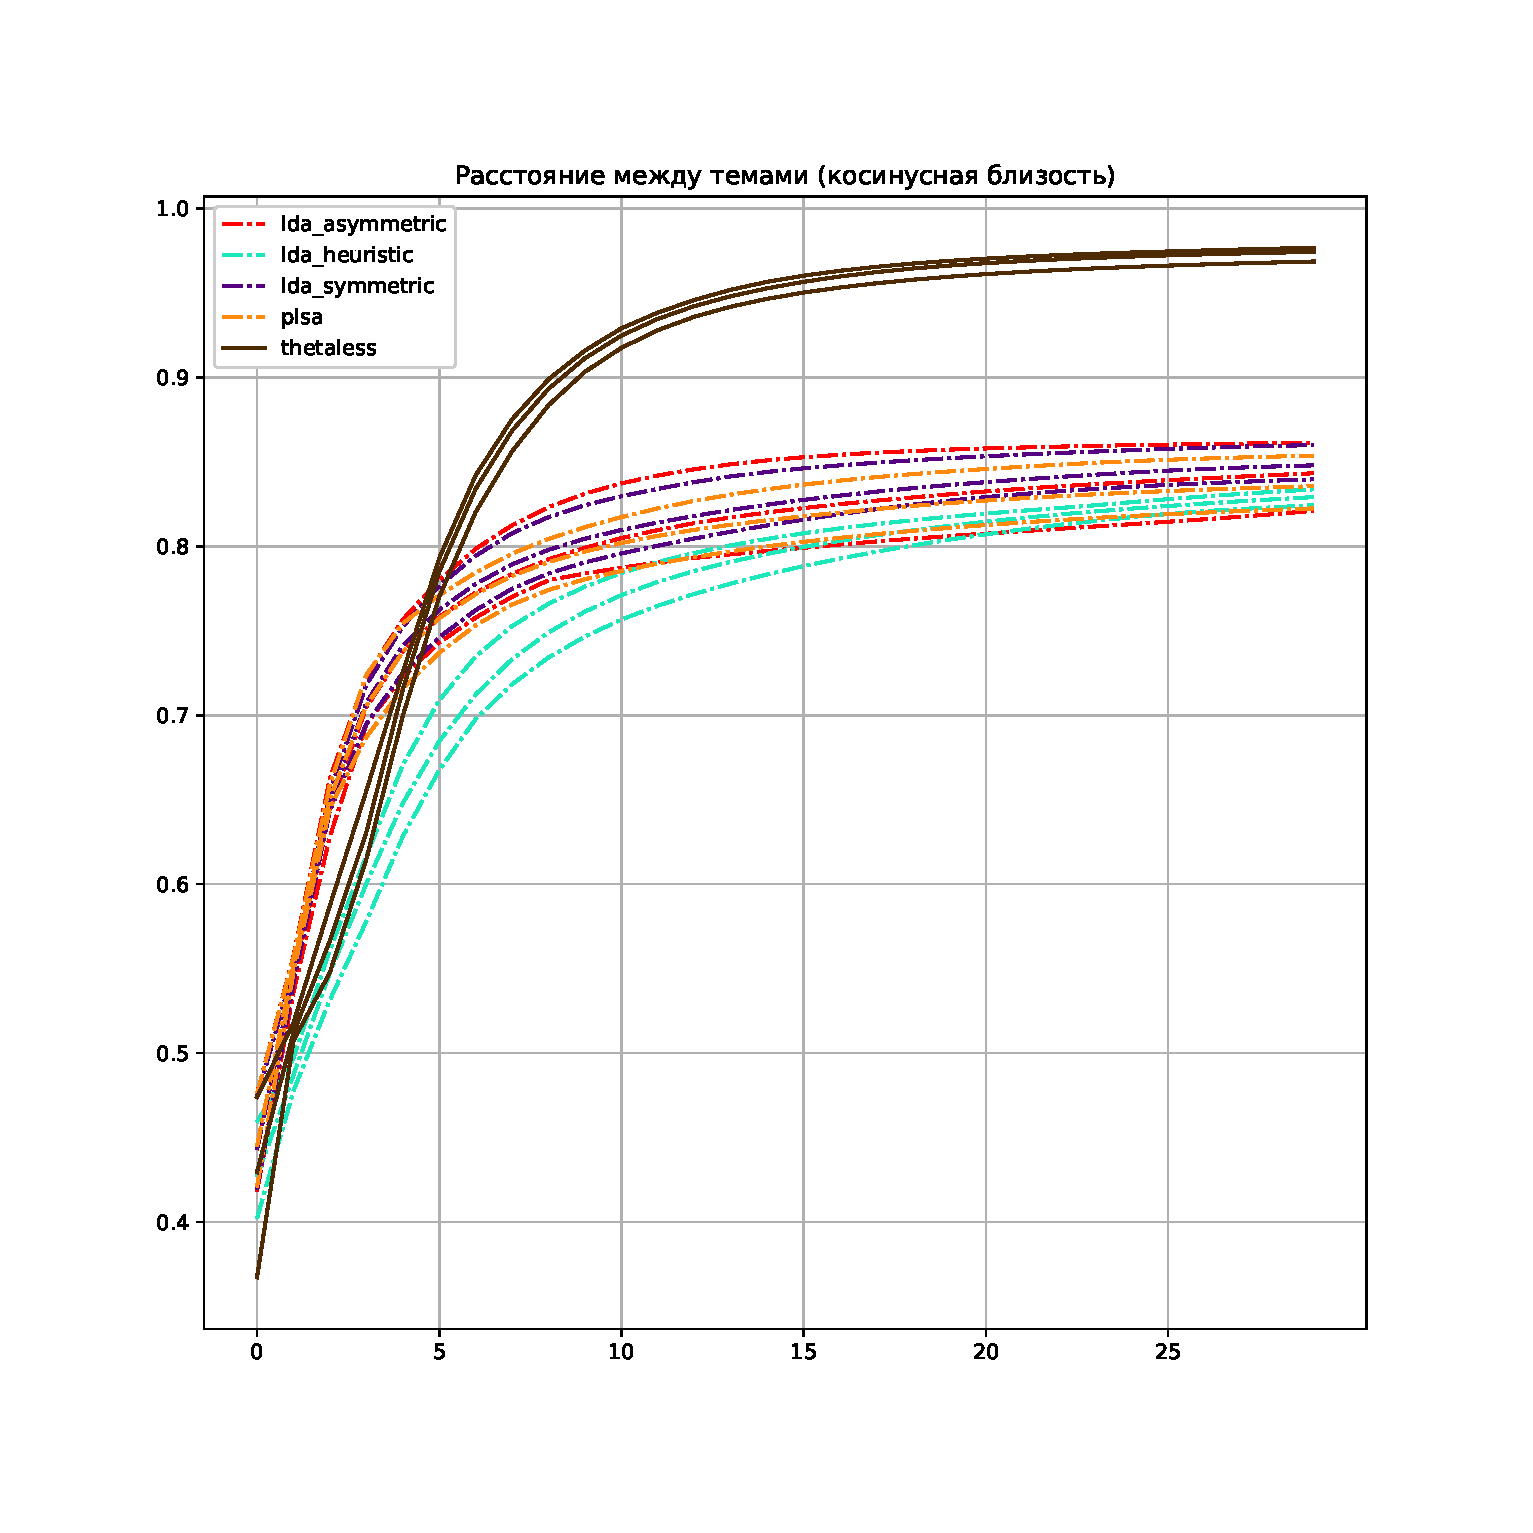
\includegraphics[width=55mm]{images/CH4_baselines_diversity_cosine_False.eps} &   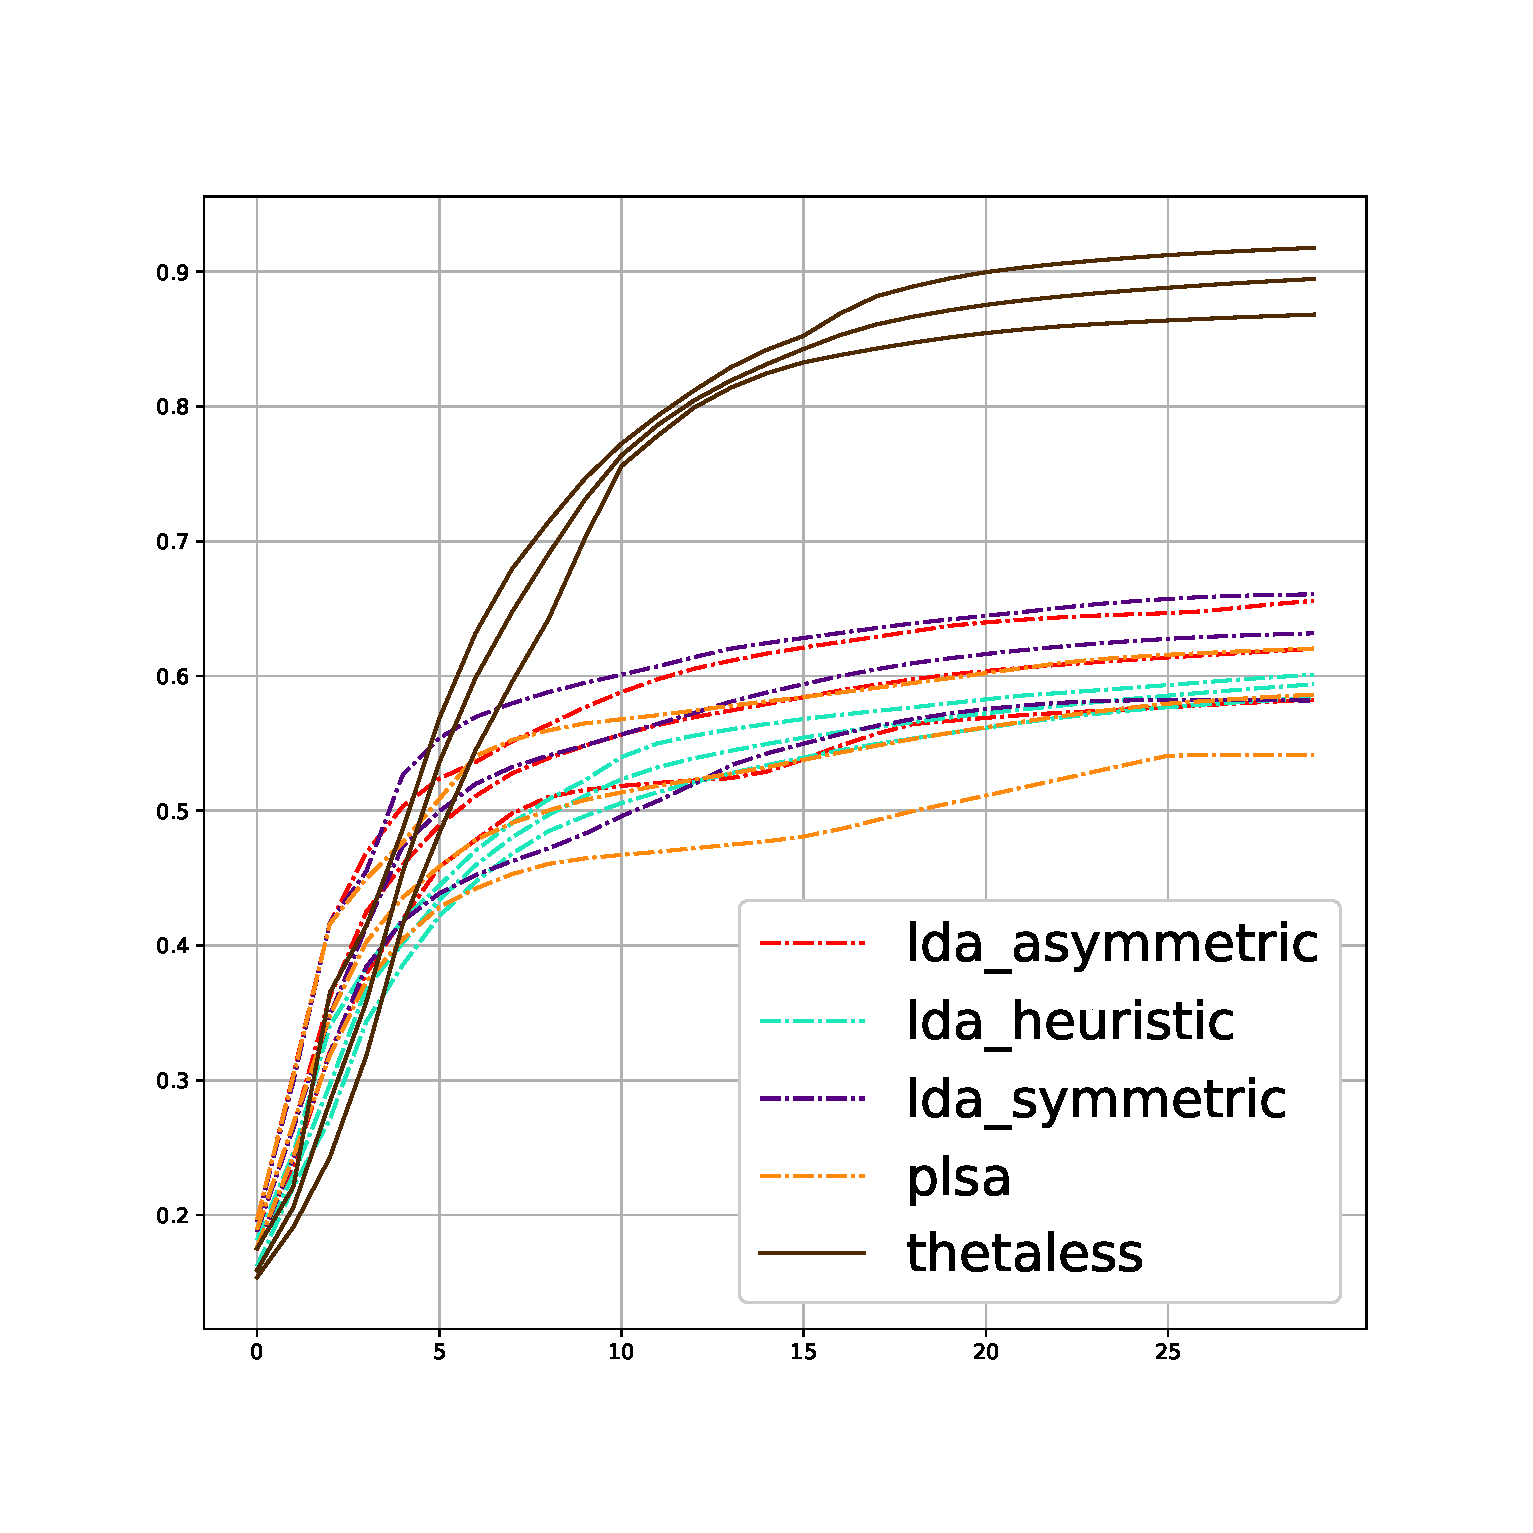
\includegraphics[width=55mm]{images/CH4_baselines_diversity_cosine_True.eps} & 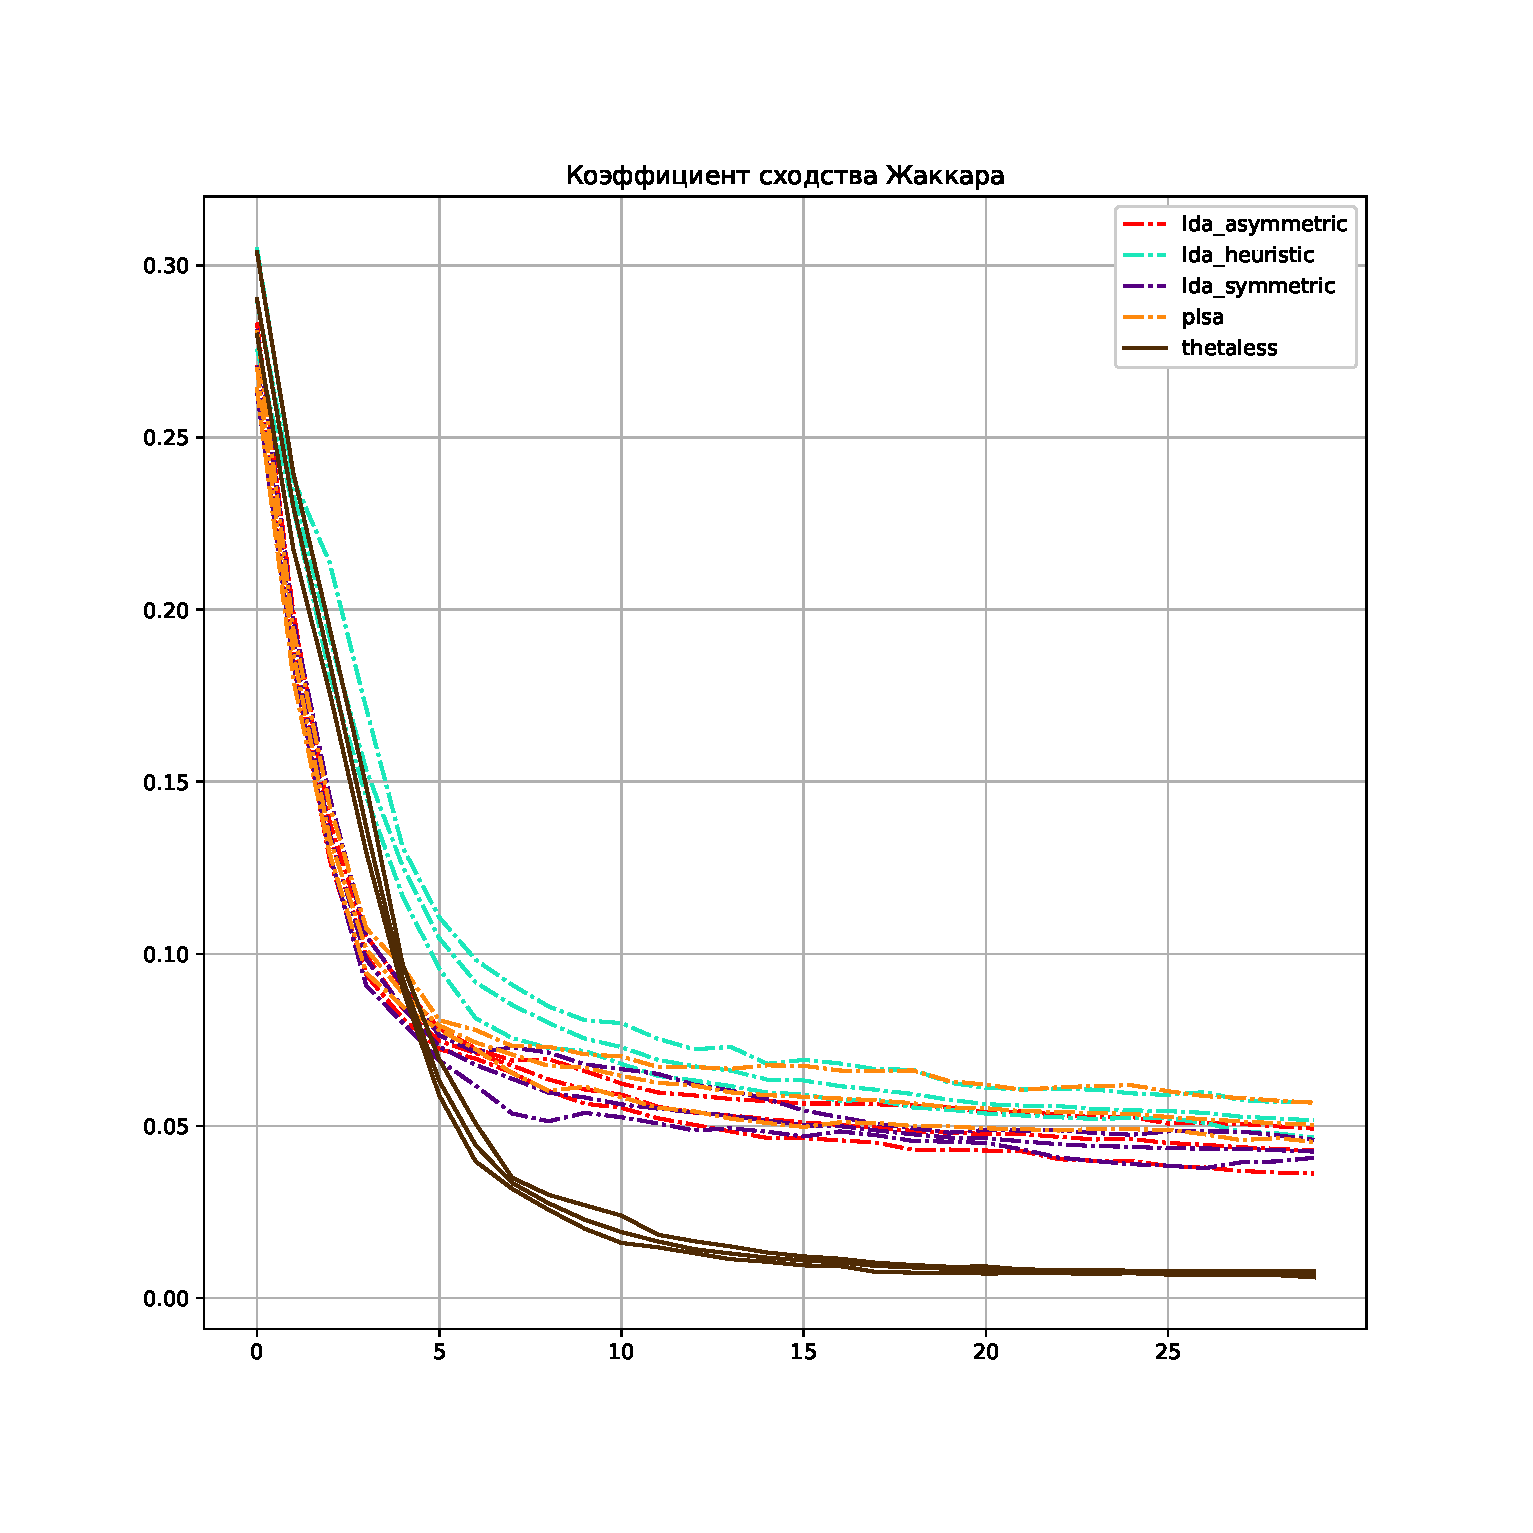
\includegraphics[width=55mm]{images/CH4_baselines_jaccard_sim_30.eps} \\
    % (a) first & (b) second & (c) third \\[6pt]
    
    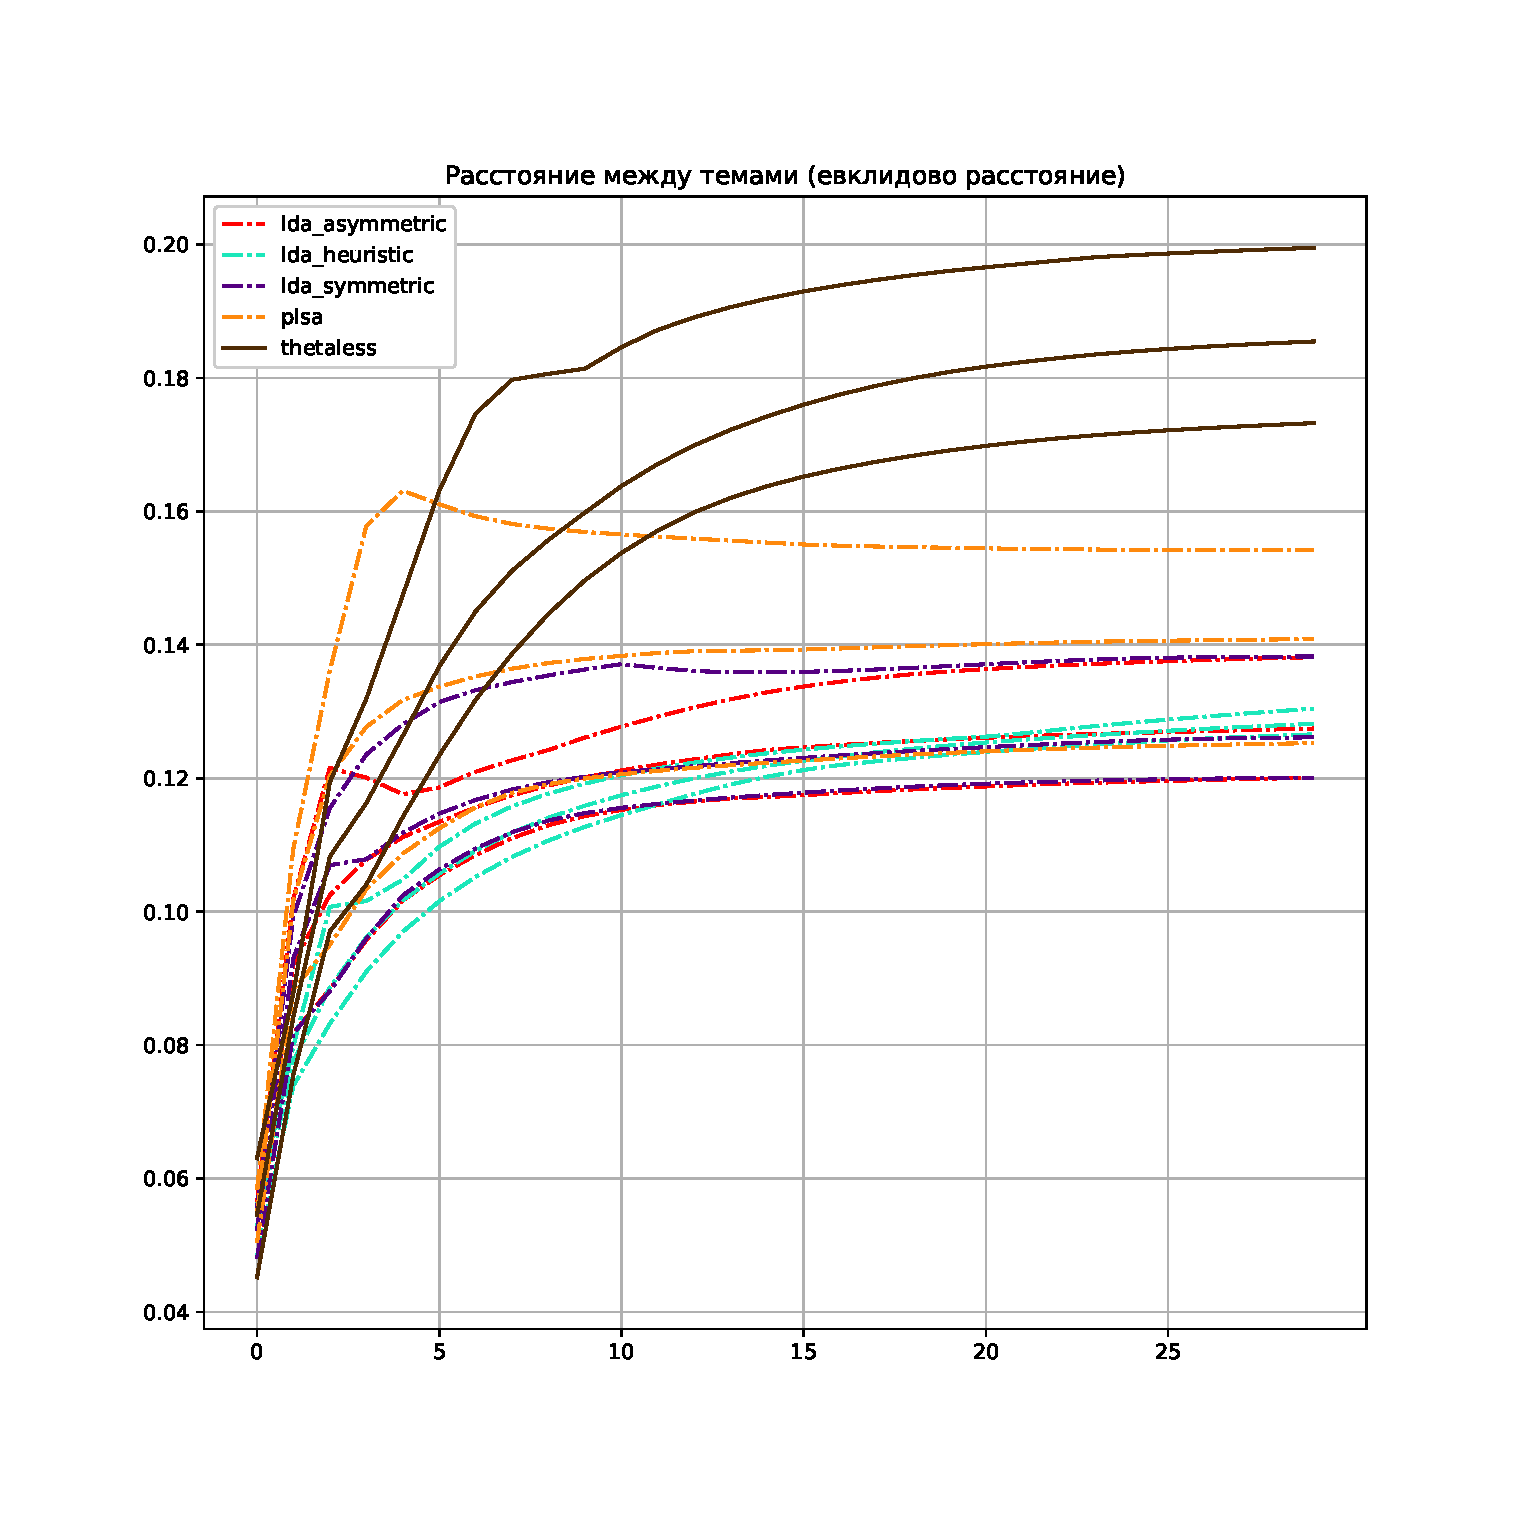
\includegraphics[width=55mm]{images/CH4_baselines_diversity_euclidean_False.eps} &   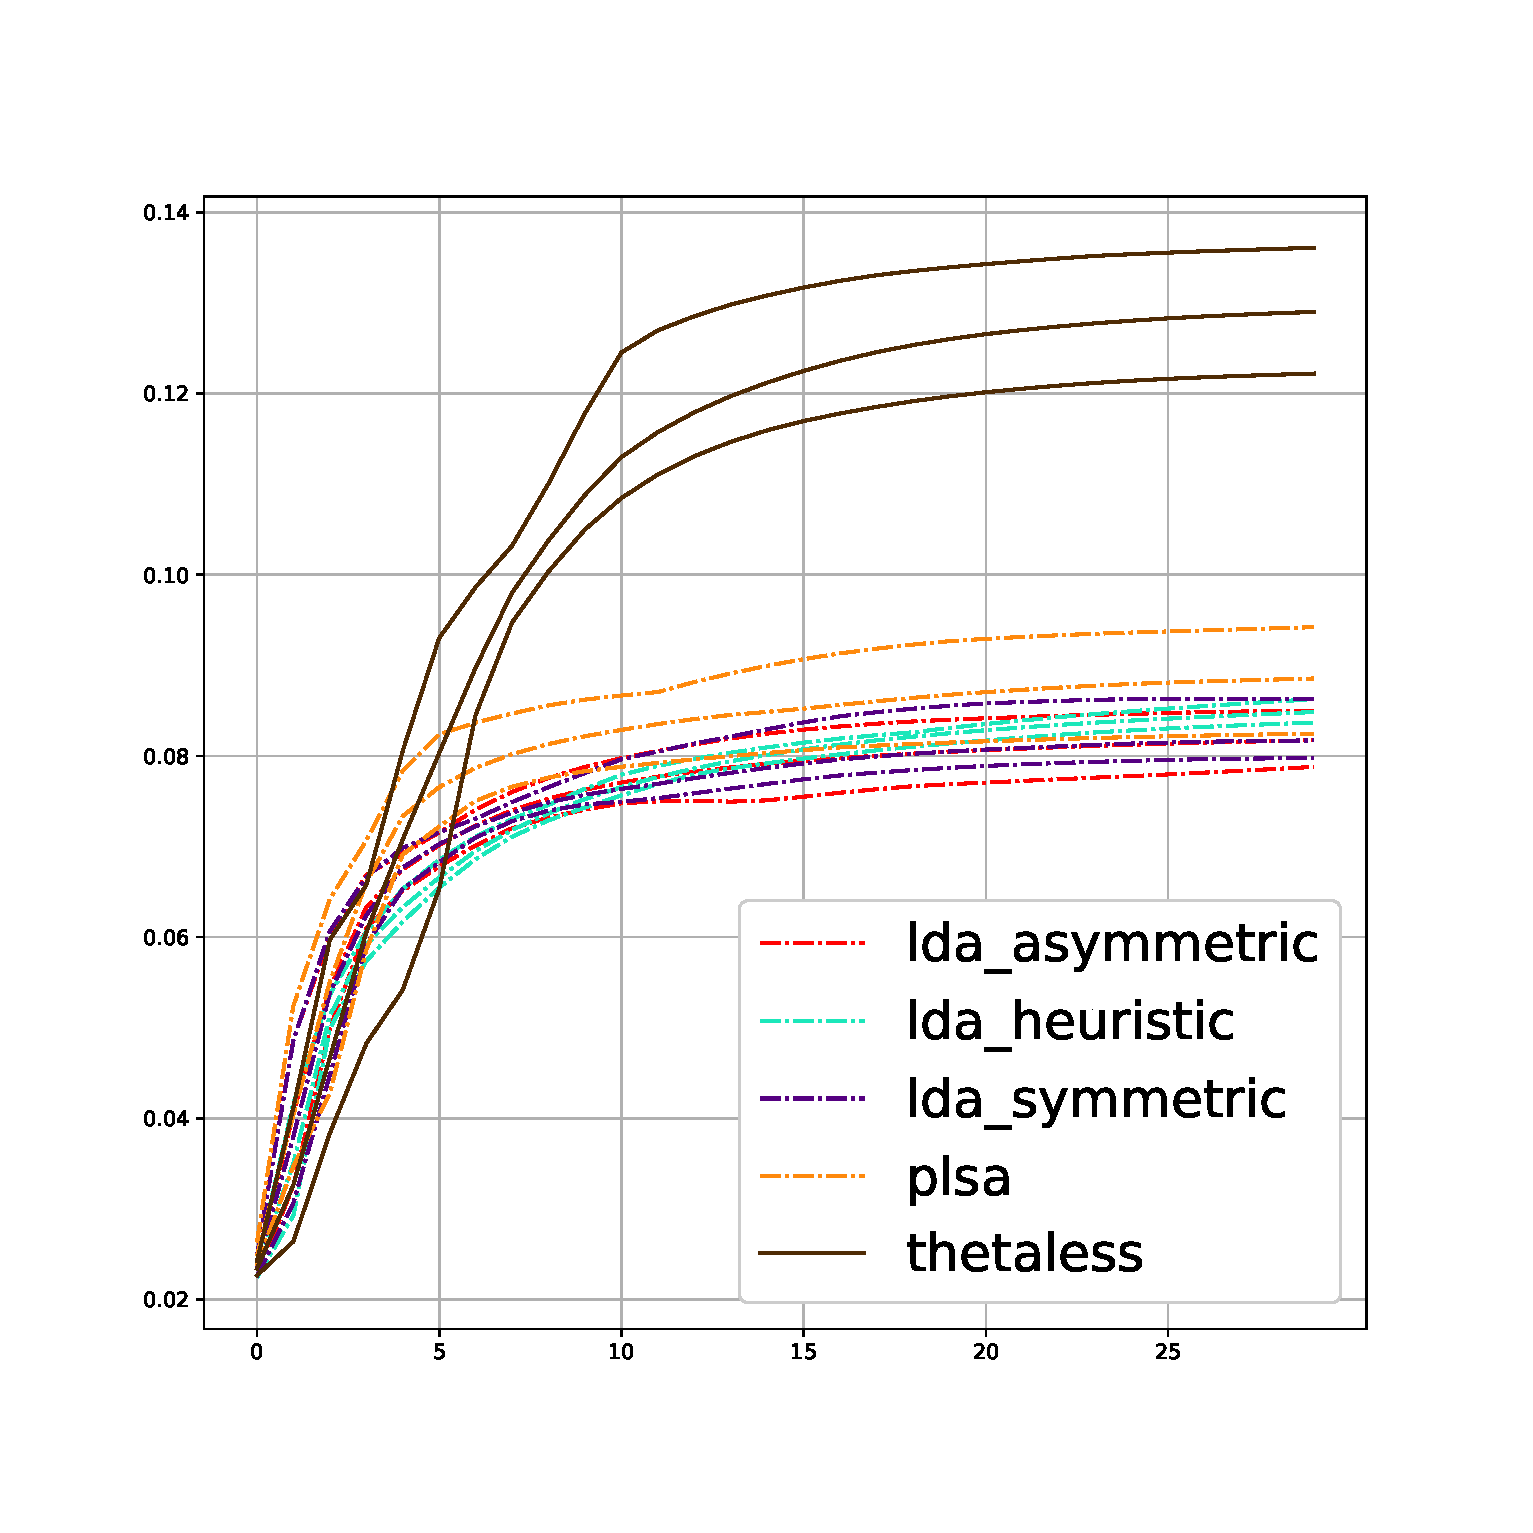
\includegraphics[width=55mm]{images/CH4_baselines_diversity_euclidean_True.eps} & 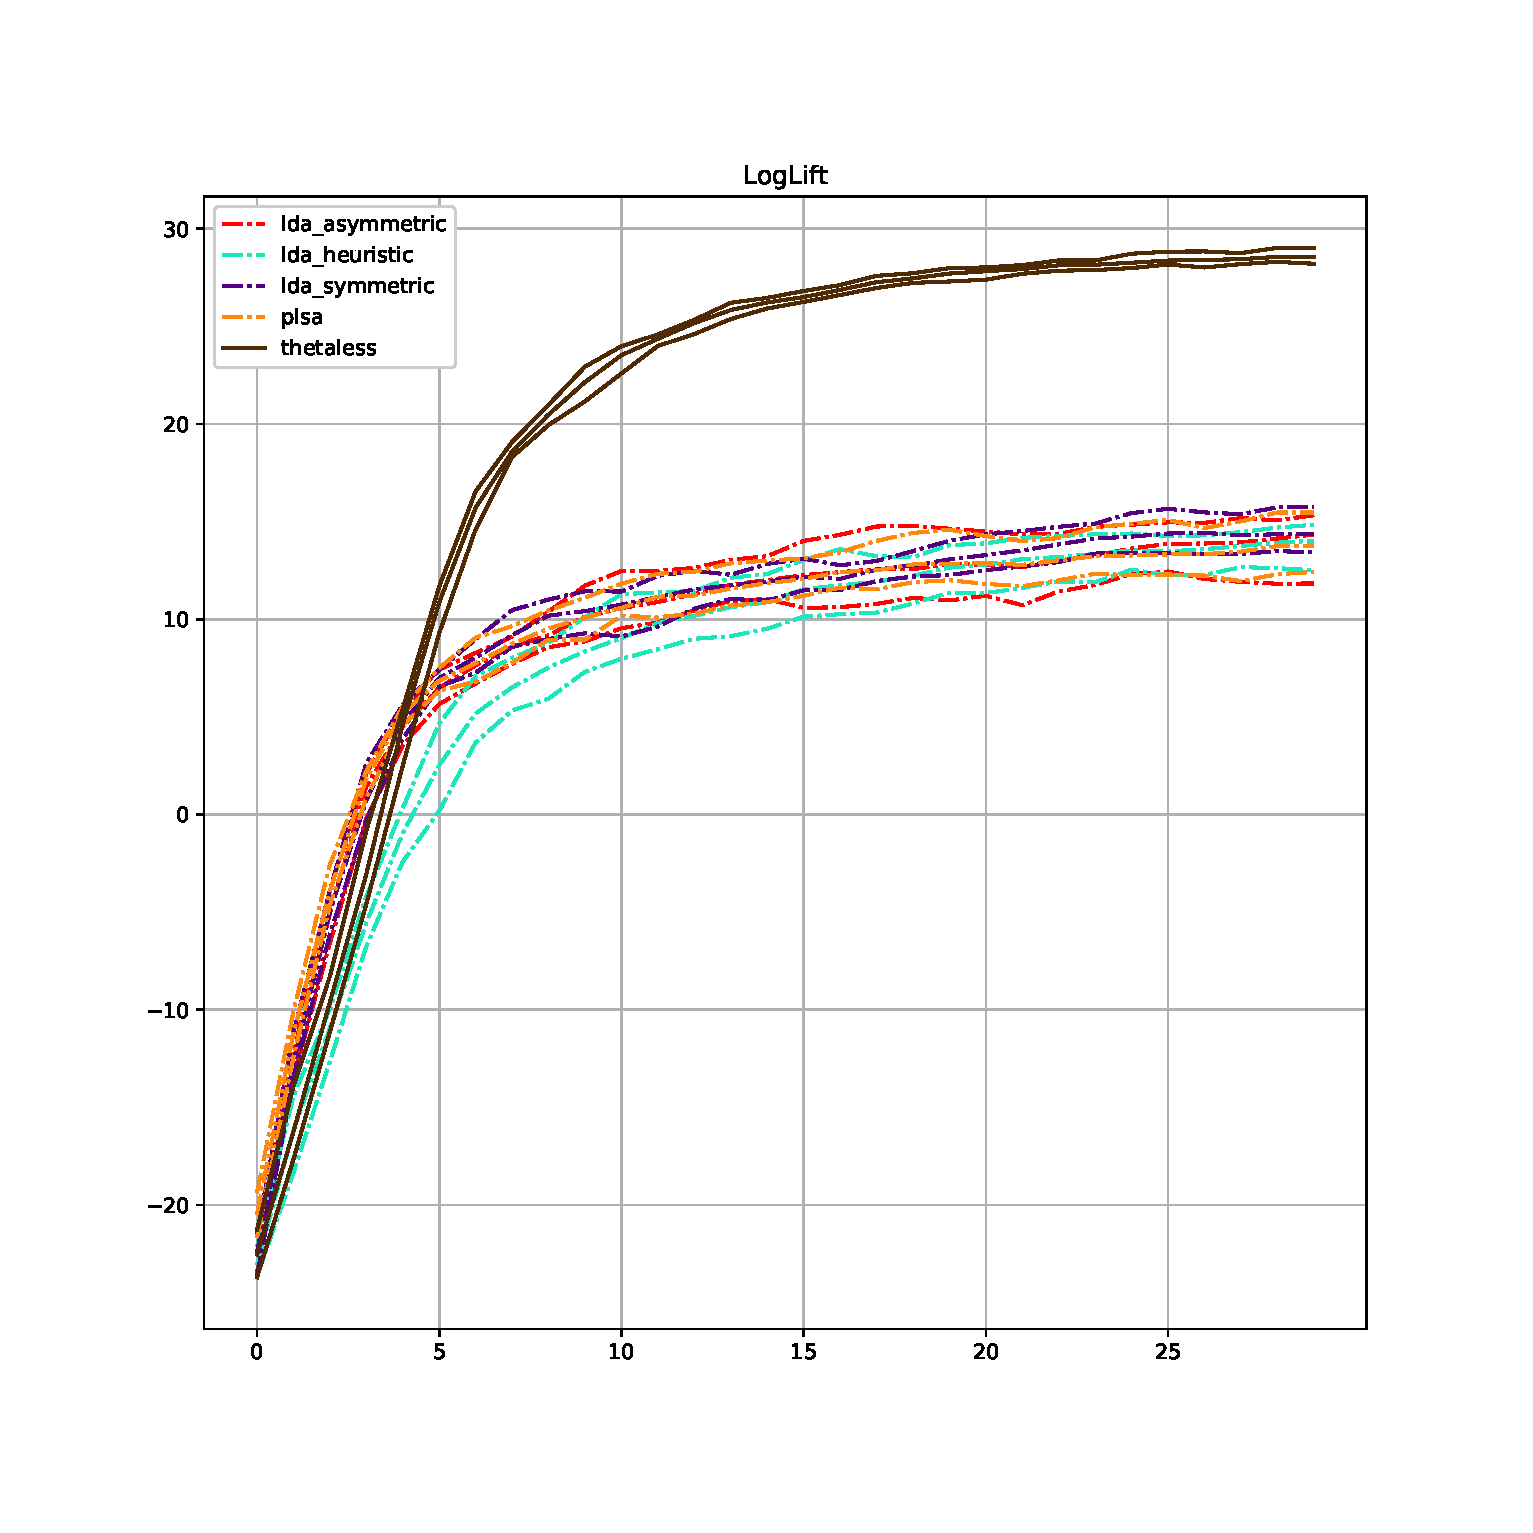
\includegraphics[width=55mm]{images/CH4_baselines_loglift30.eps} \\
    % (a) first & (b) second & (c) third \\[6pt]
    
    
    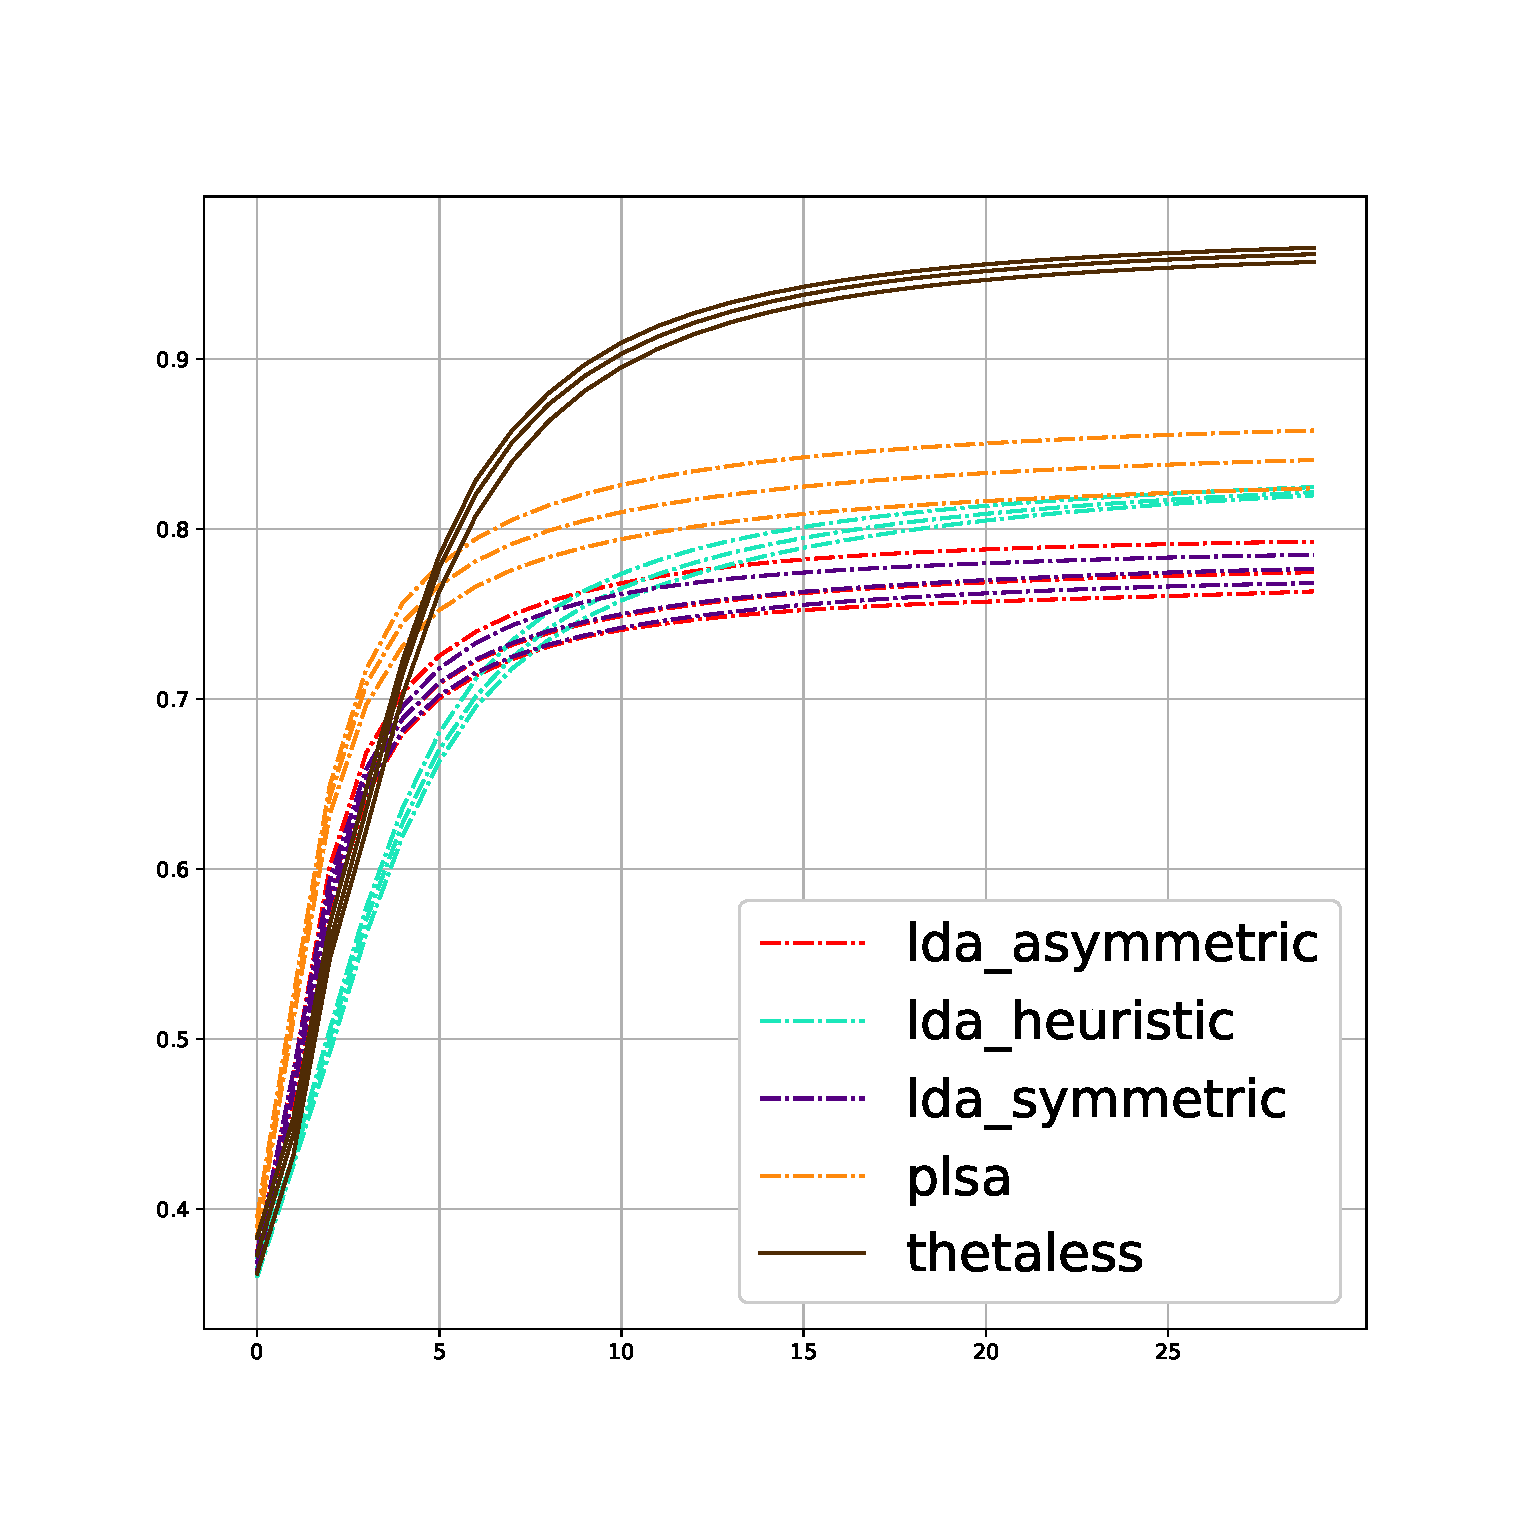
\includegraphics[width=55mm]{images/CH4_baselines_diversity_hellinger_False.eps} &   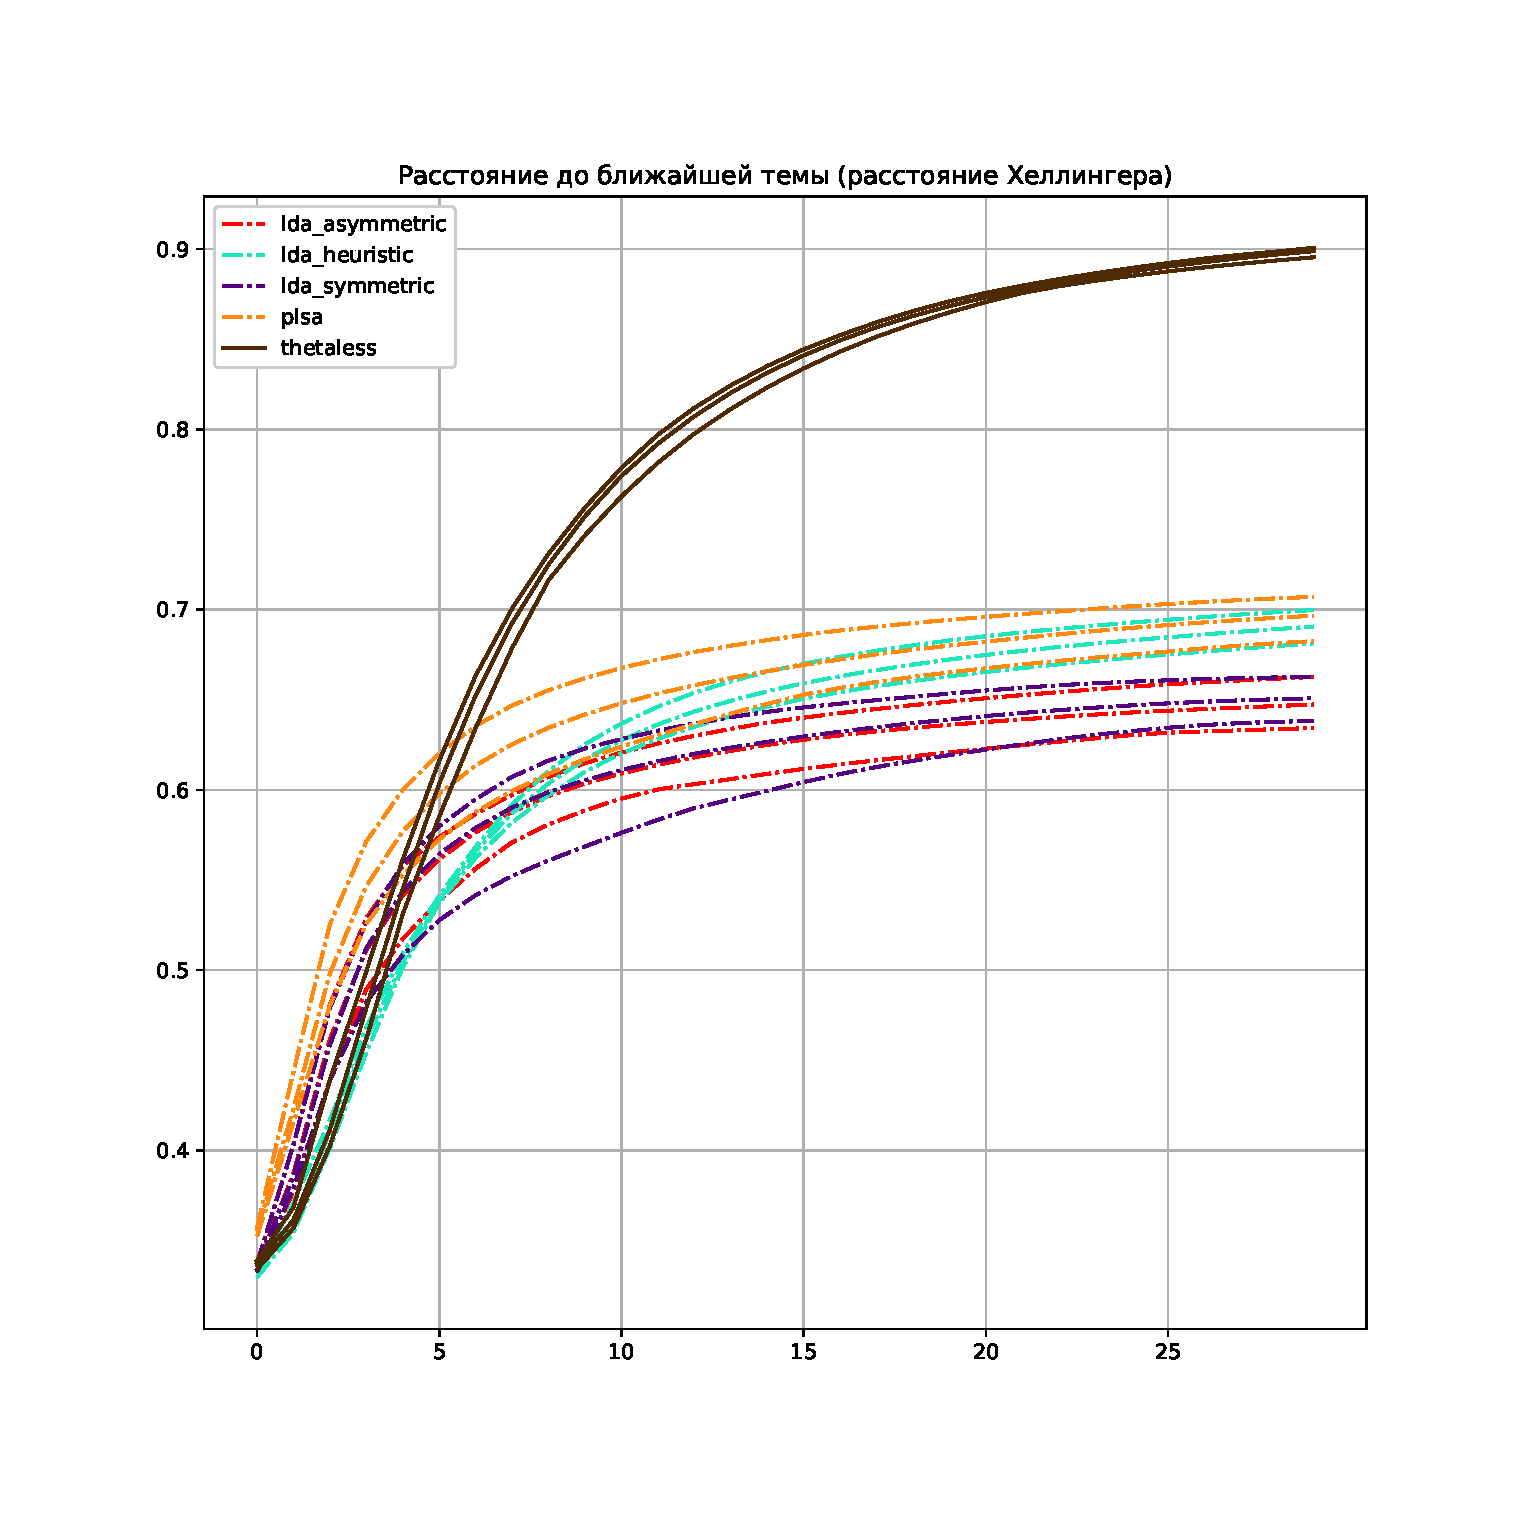
\includegraphics[width=55mm]{images/CH4_baselines_diversity_hellinger_True.eps} & 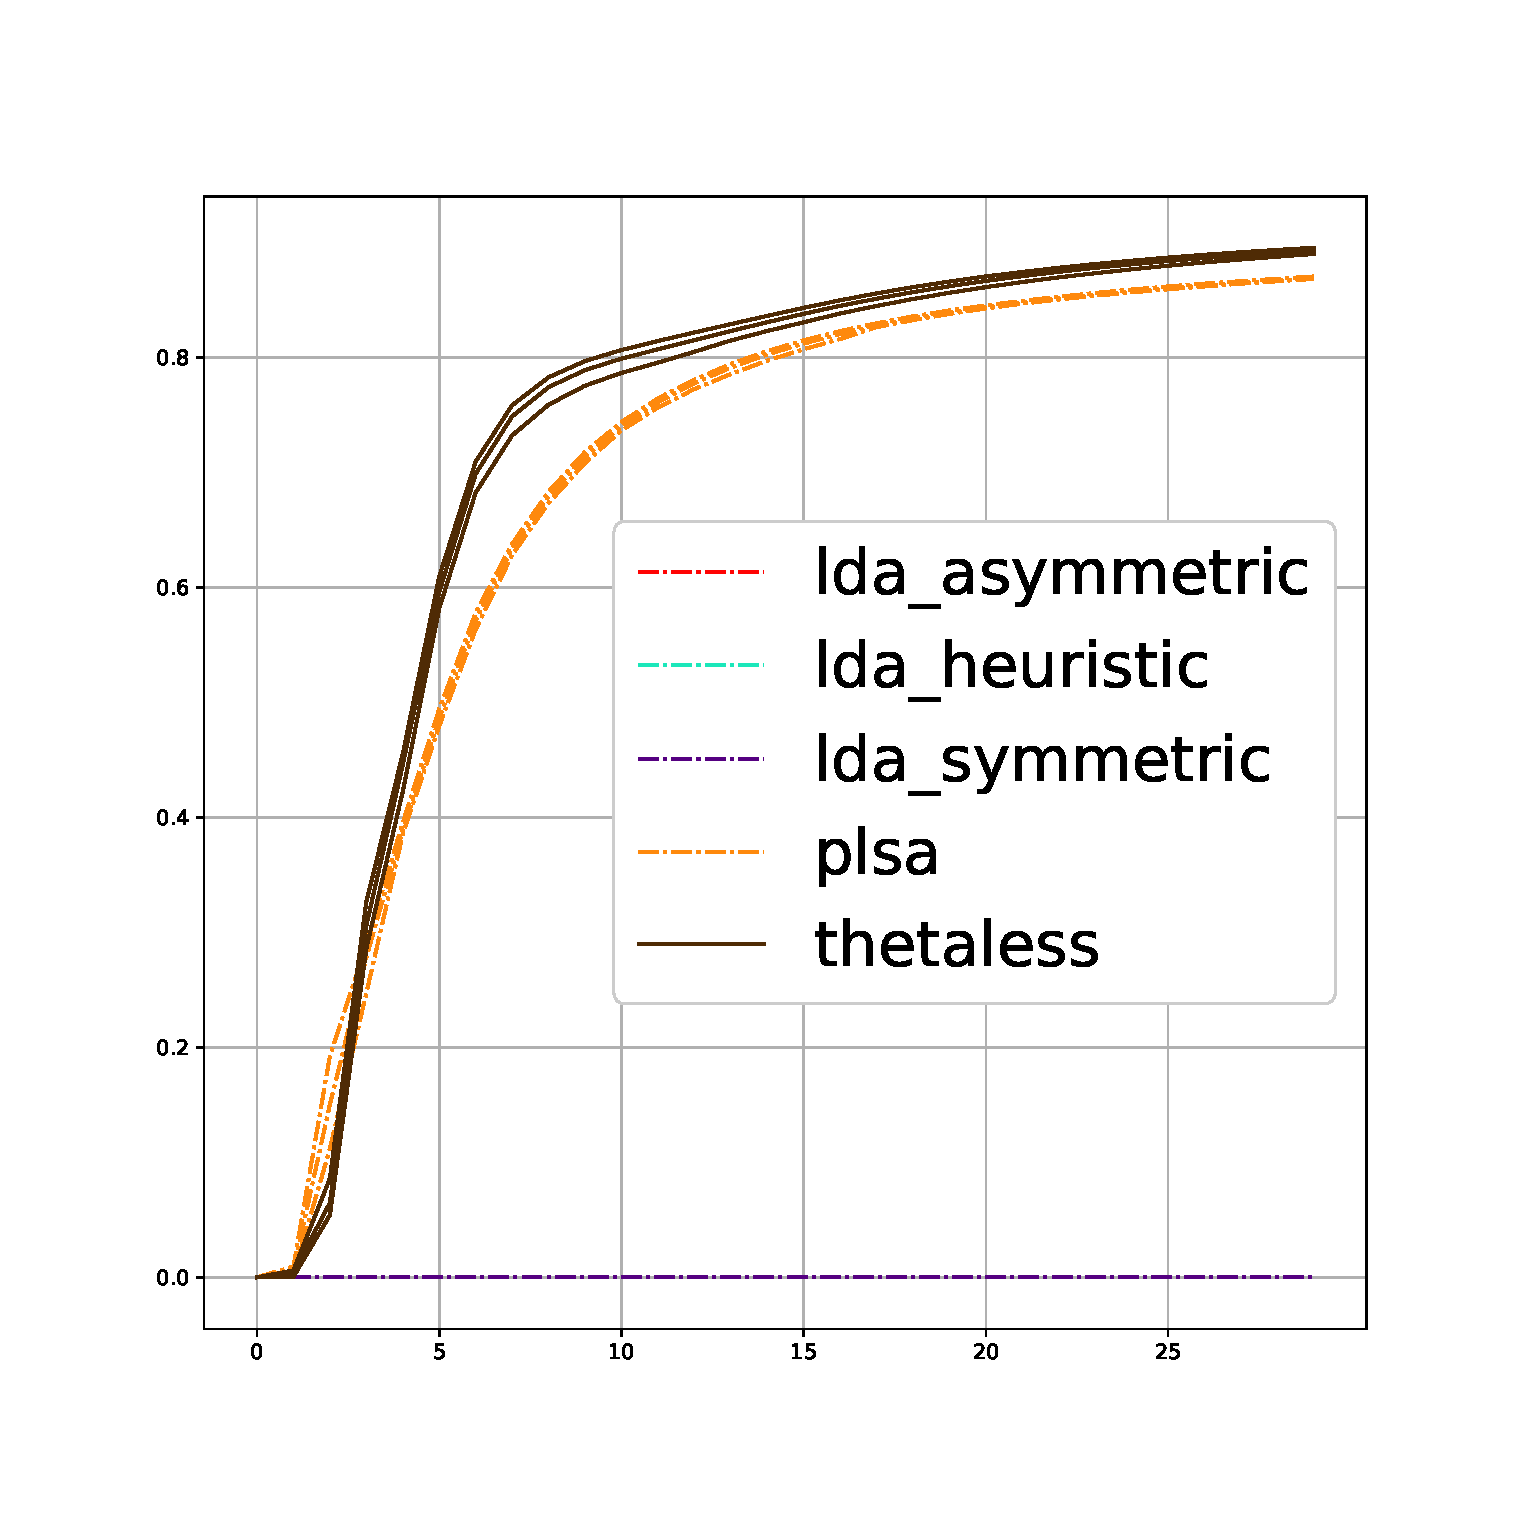
\includegraphics[width=55mm]{images/CH4_baselines_SparsityPhiScore.eps} \\
    % (a) first & (b) second & (c) third \\[6pt]
    
    
    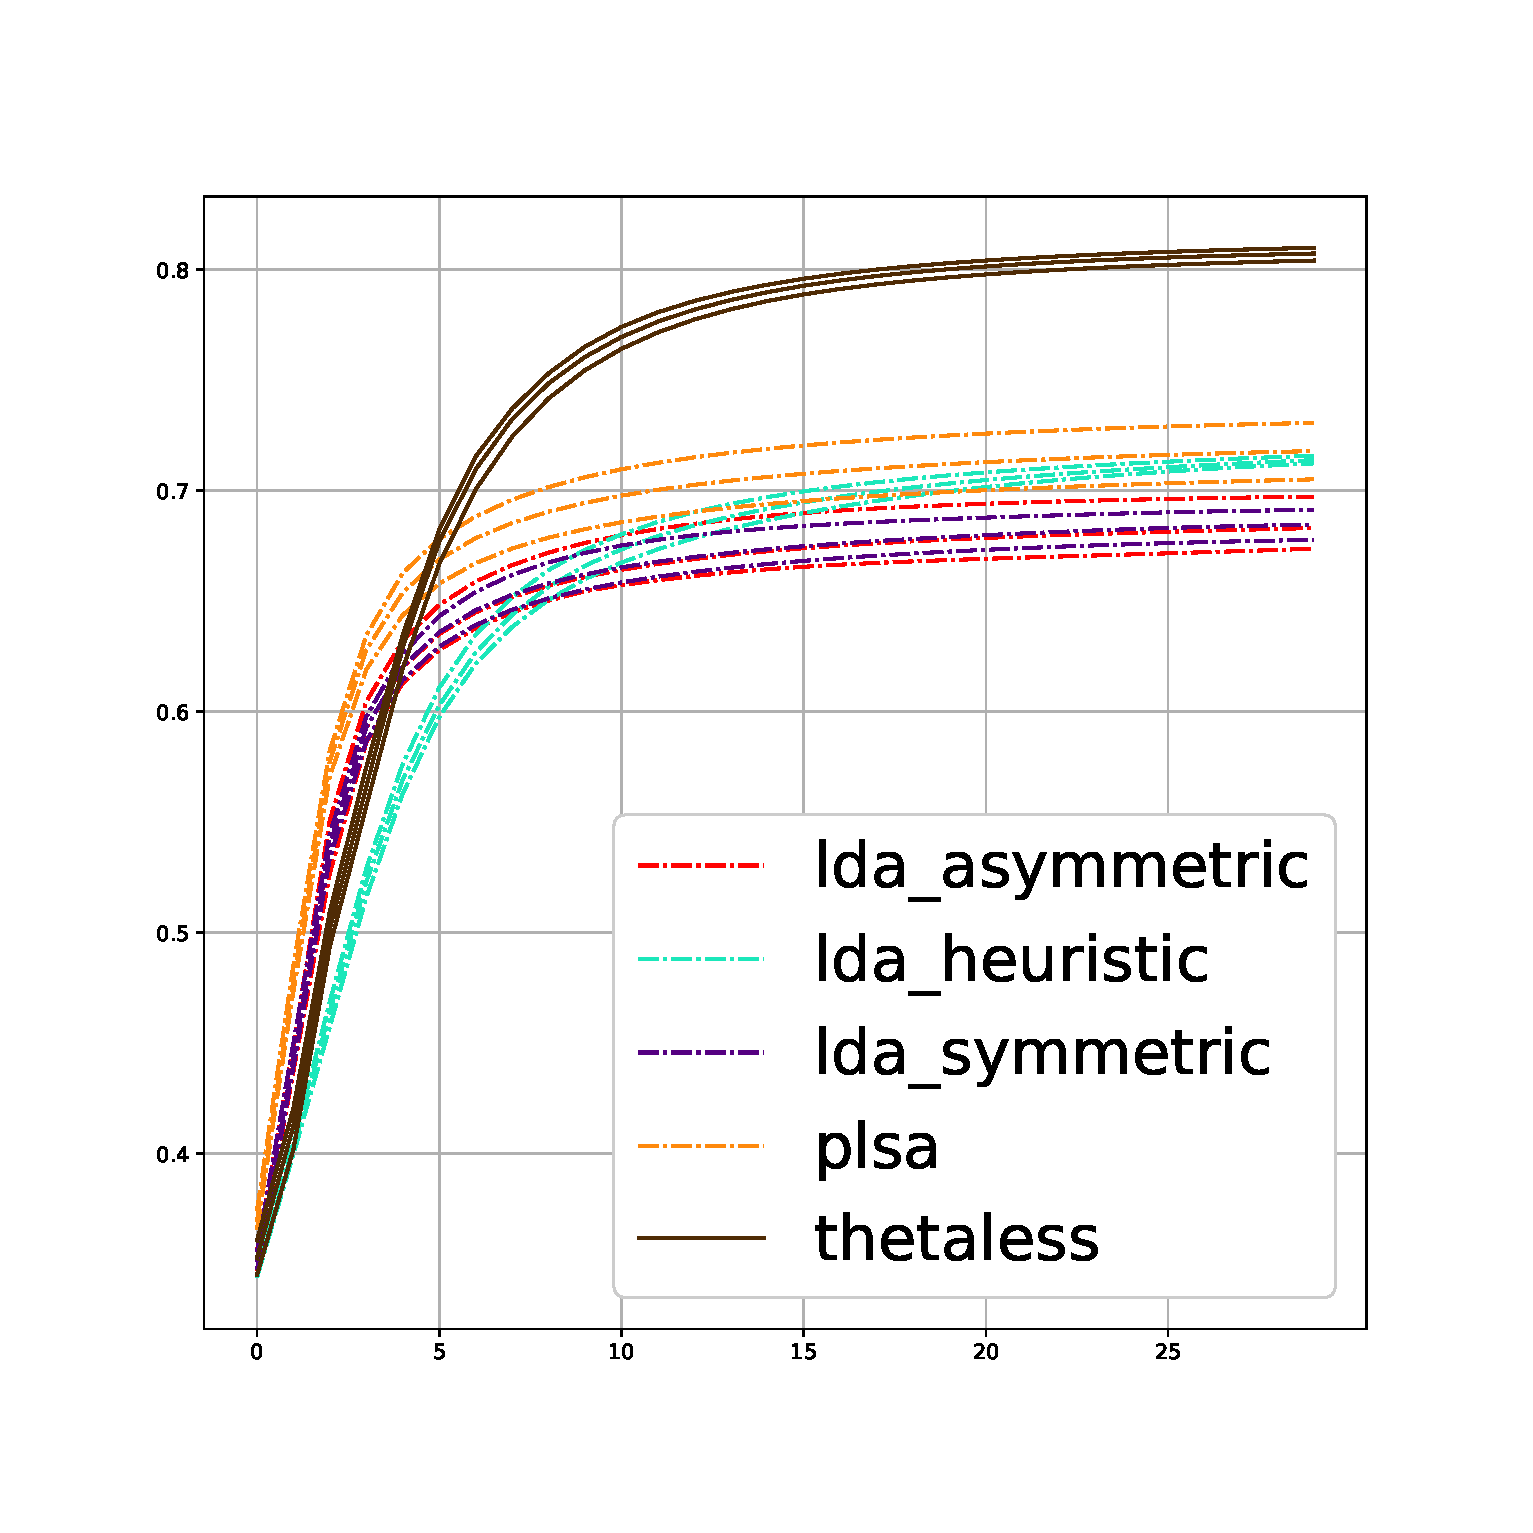
\includegraphics[width=55mm]{images/CH4_baselines_diversity_jensenshannon_False.eps} &   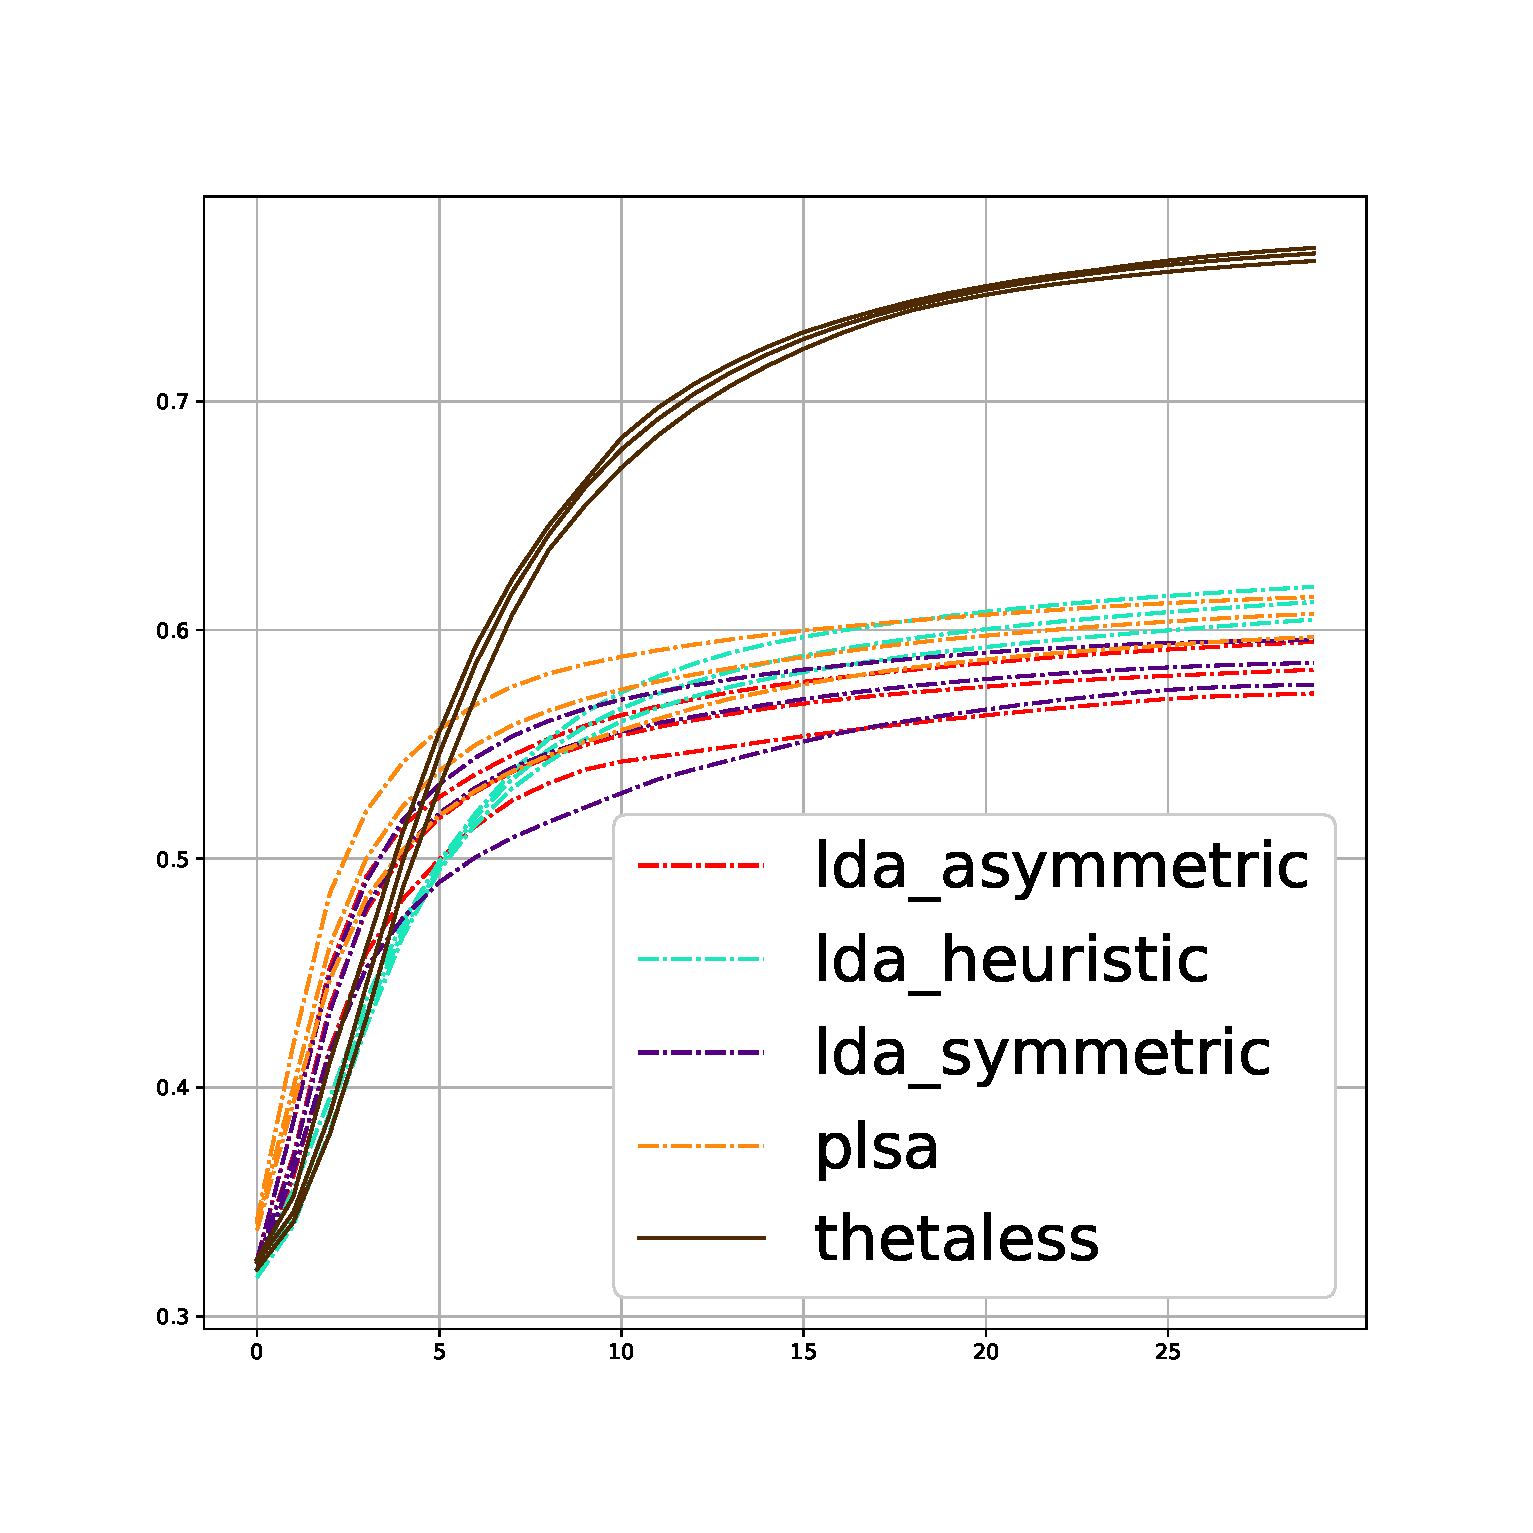
\includegraphics[width=55mm]{images/CH4_baselines_diversity_jensenshannon_True.eps} & 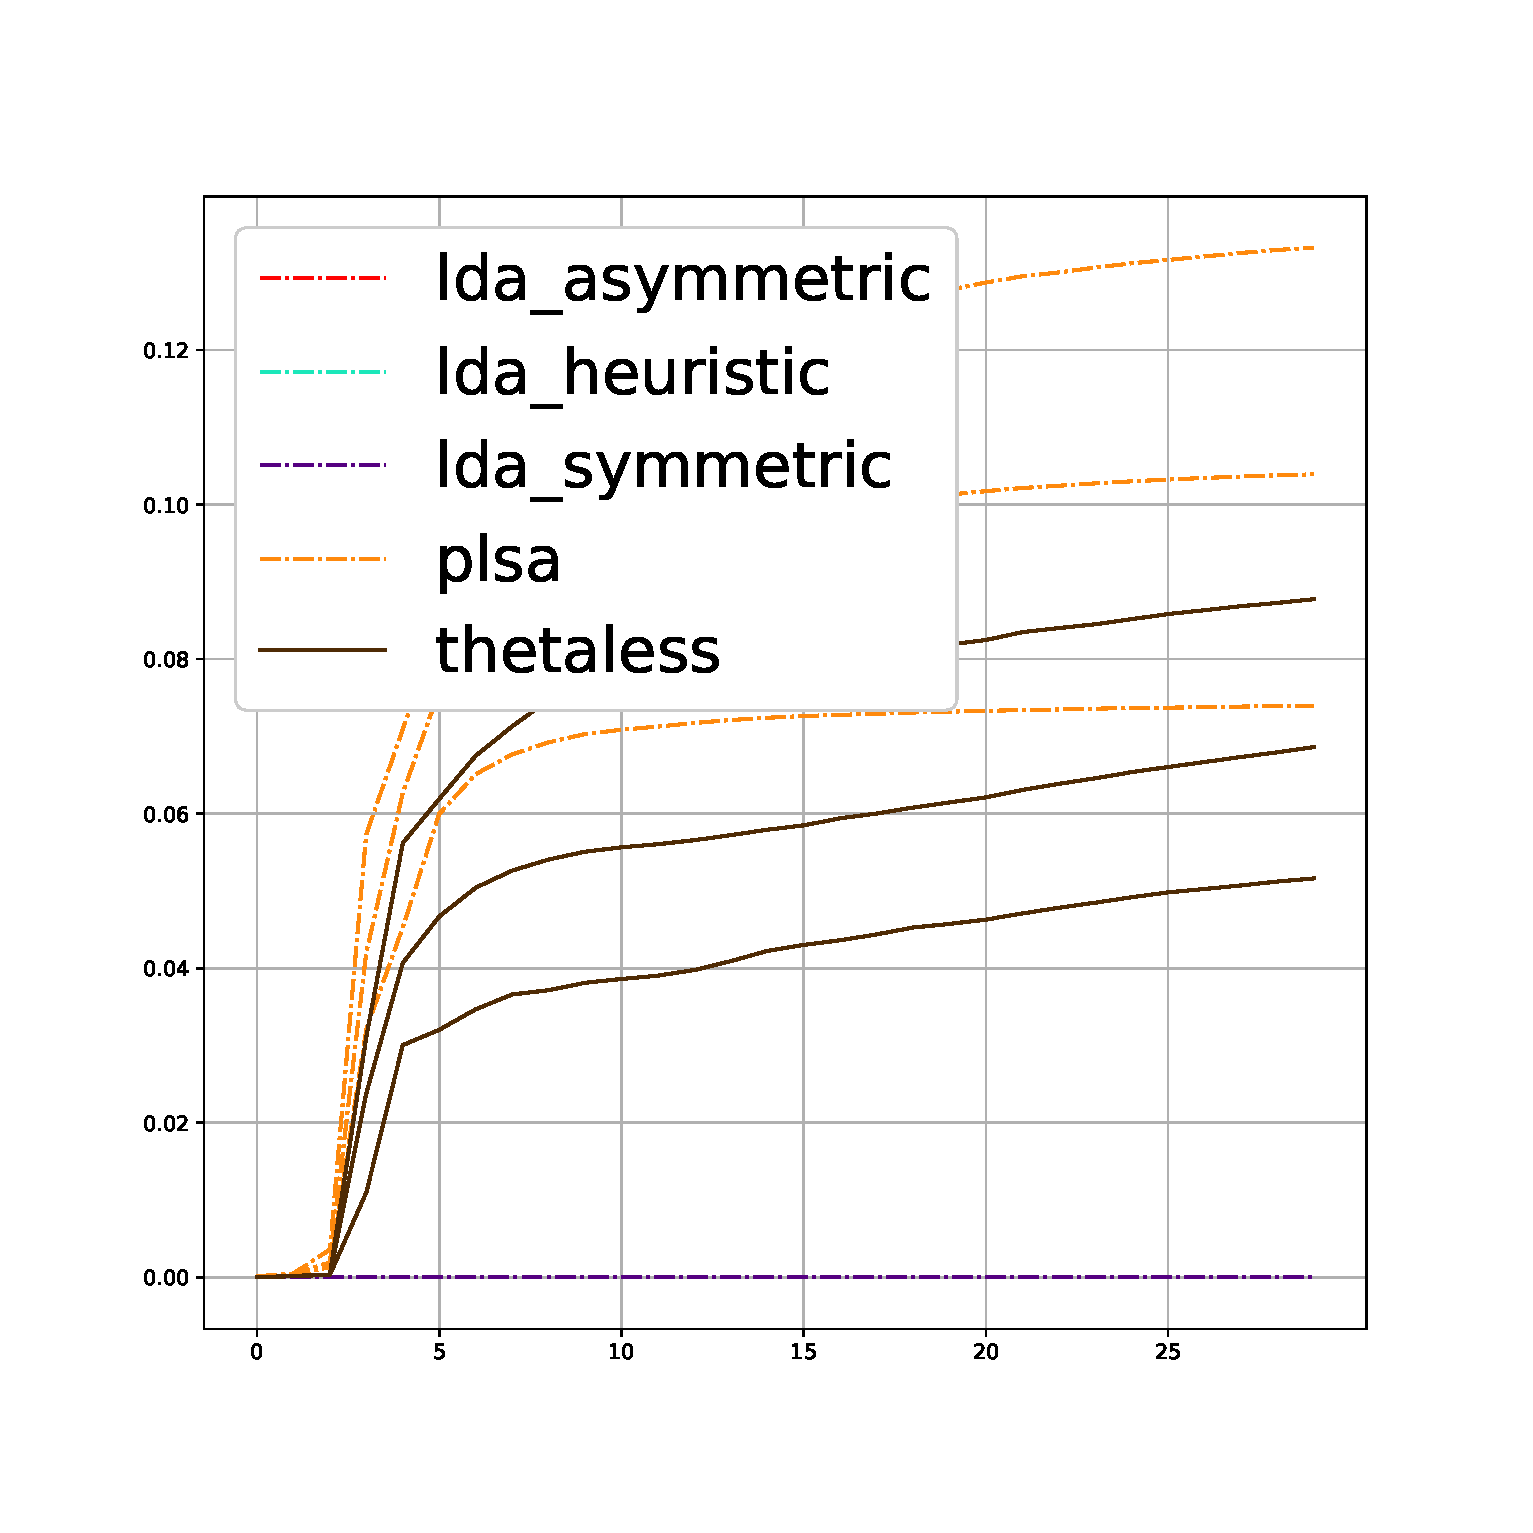
\includegraphics[width=55mm]{images/CH4_baselines_SparsityThetaScore.eps} \\
    % (a) first & (b) second & (c) third \\[6pt]
    
    %\includegraphics[width=65mm]{it} &   \includegraphics[width=65mm]{it} \\
    %(c) third & (d) fourth \\[6pt]
    
    %\multicolumn{2}{c}{\includegraphics[width=65mm]{it} }\\
    %\multicolumn{2}{c}{(e) fifth}
\end{tabular}
    \caption{Графики зависимости различных критериев качества тематических моделей для пяти моделей (TARTM, PLSA, LDA с 3 видами приоров). Каждой модели соответствуют три линии: среднее значение, минимум и максимум (по пяти случайным перезапускам).}
\label{fig:ch4_base}
\end{figure}


\begin{figure}
\begin{tabular}{ccc}
    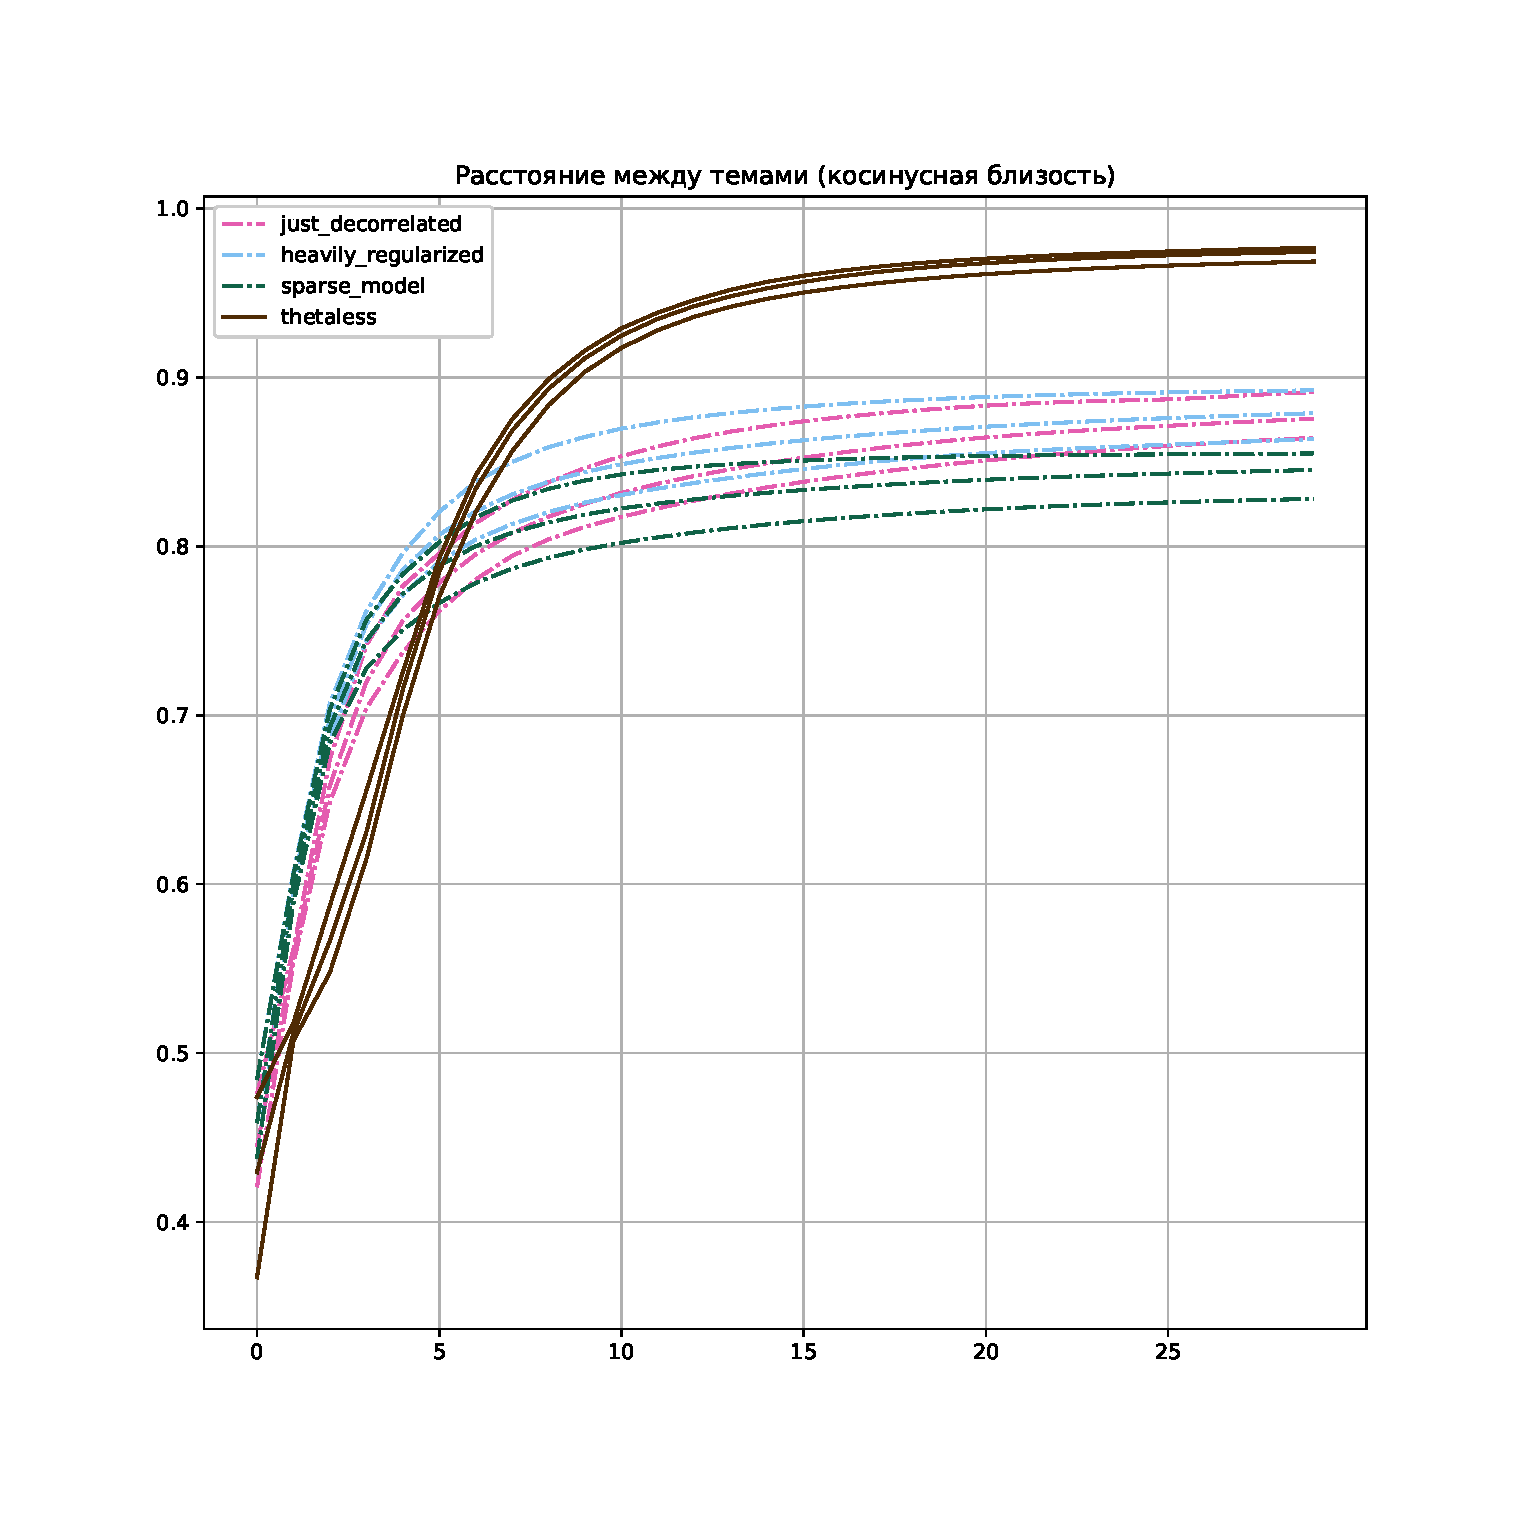
\includegraphics[width=55mm]{images/CH4_vs_regularized_diversity_cosine_False.eps} &   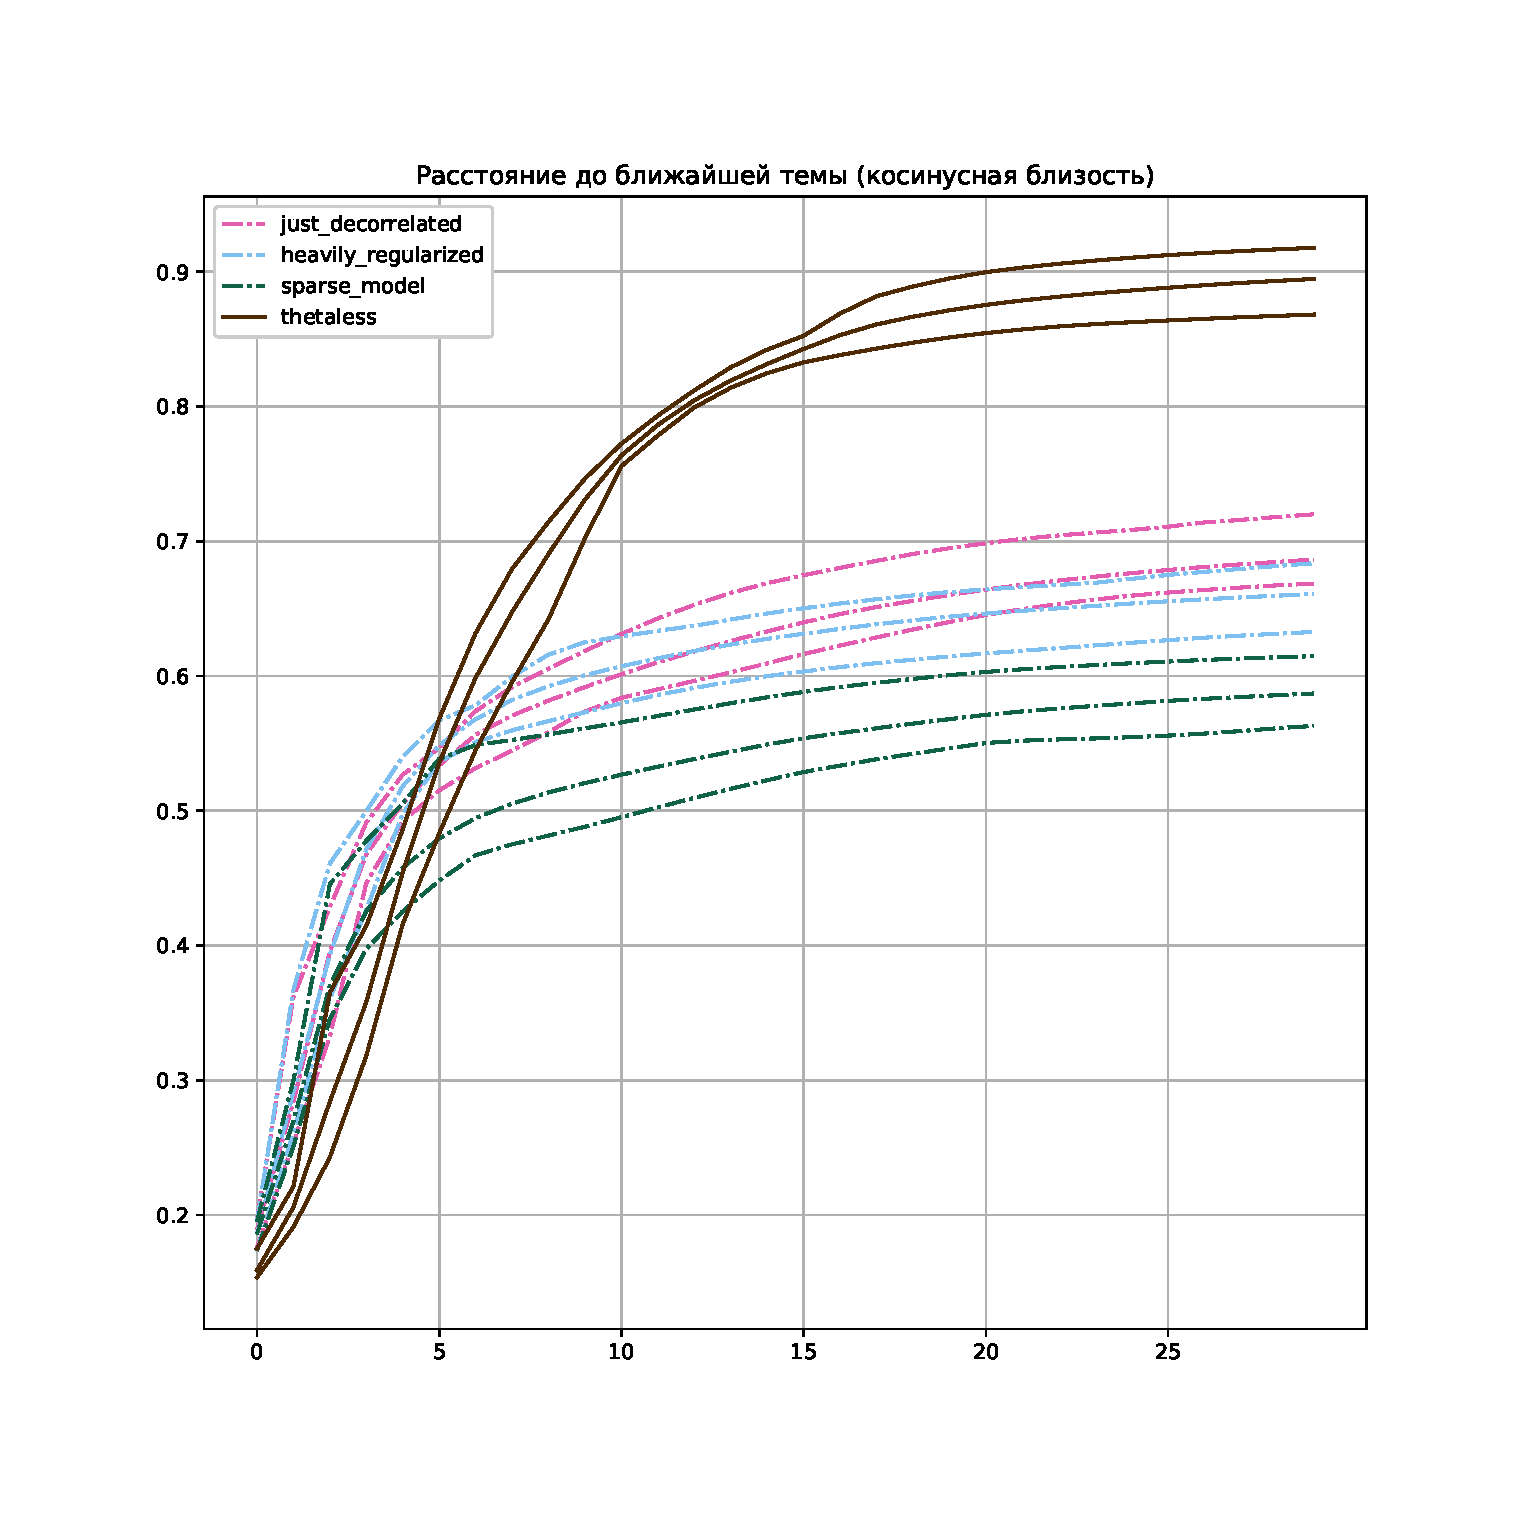
\includegraphics[width=55mm]{images/CH4_vs_regularized_diversity_cosine_True.eps} & 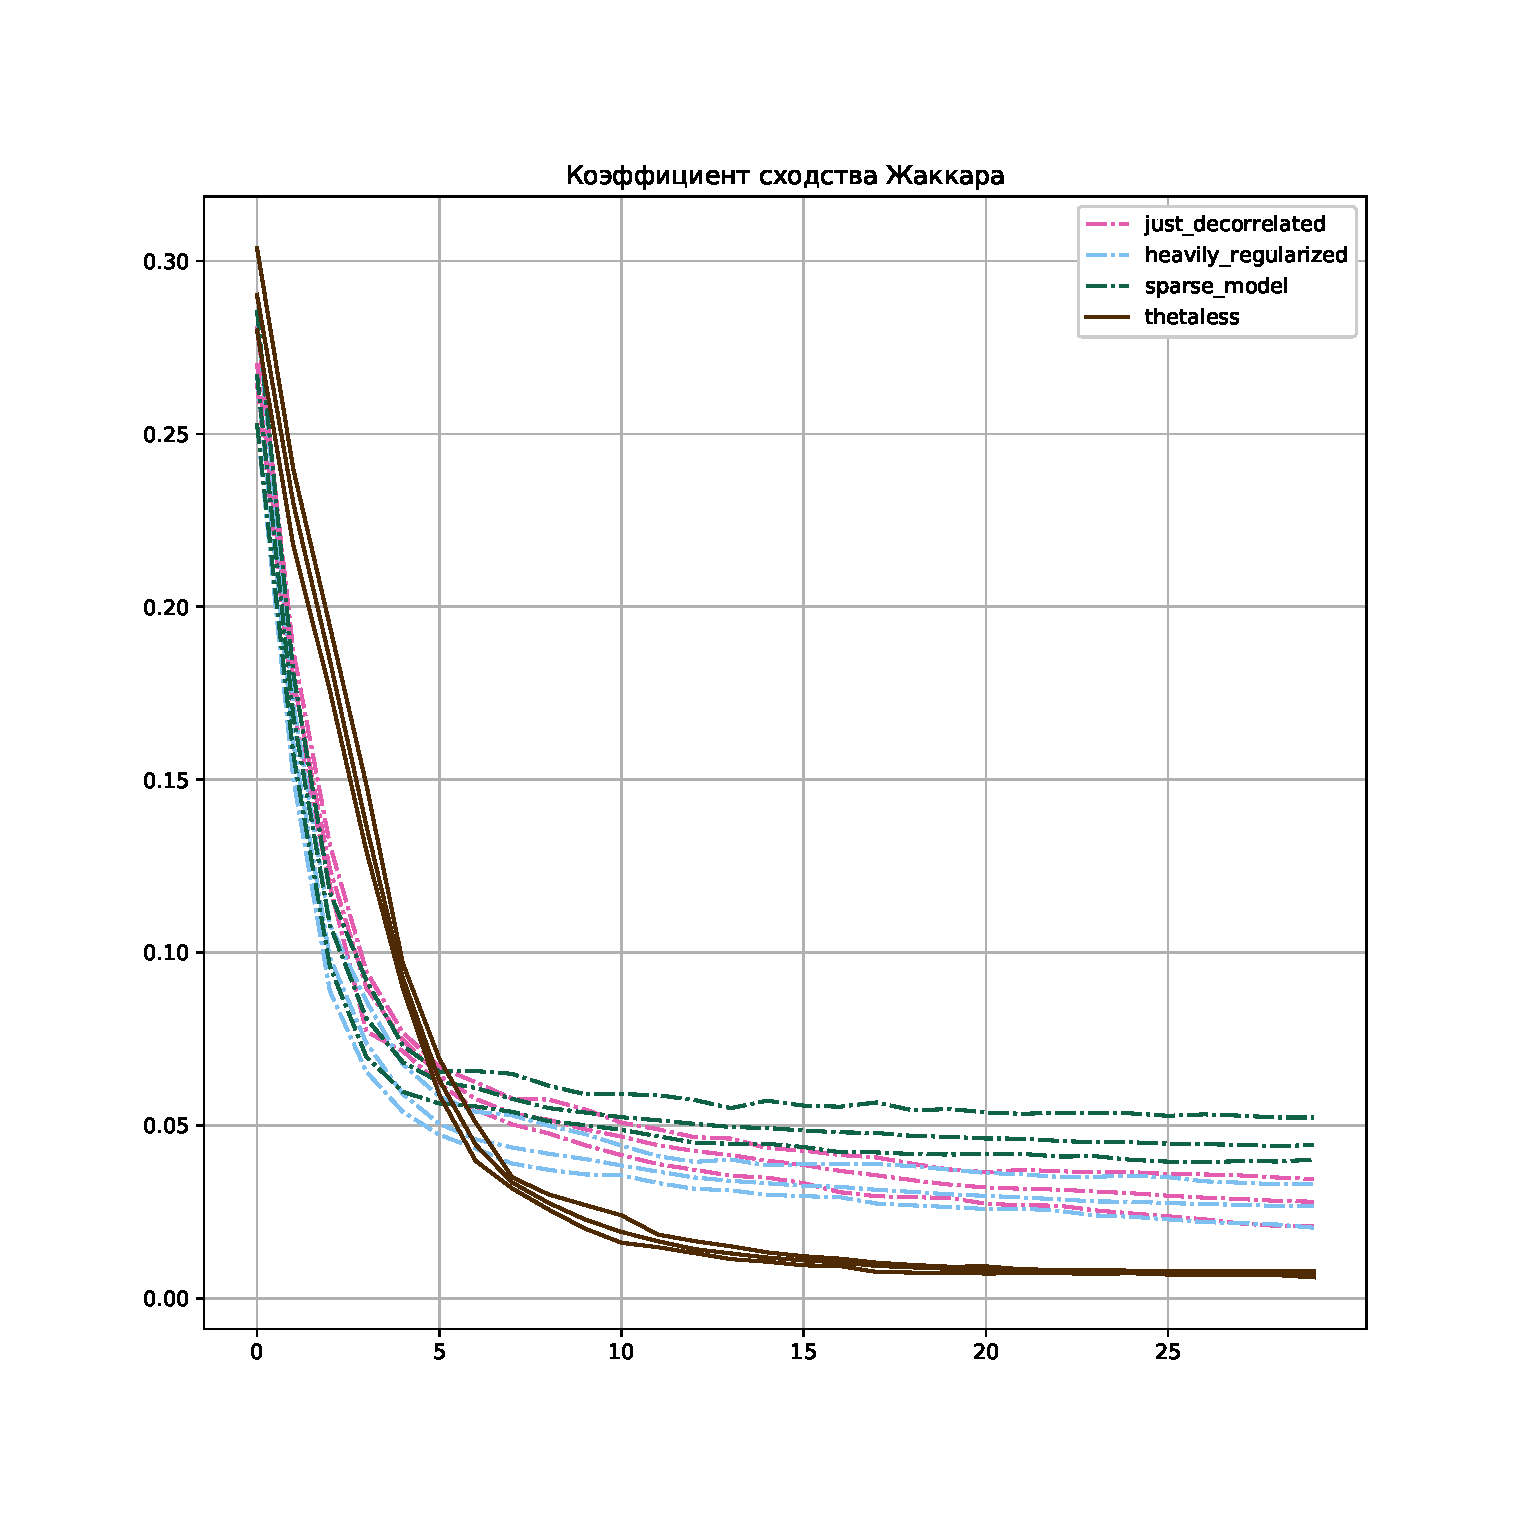
\includegraphics[width=55mm]{images/CH4_vs_regularized_jaccard_sim_30.eps} \\
    
    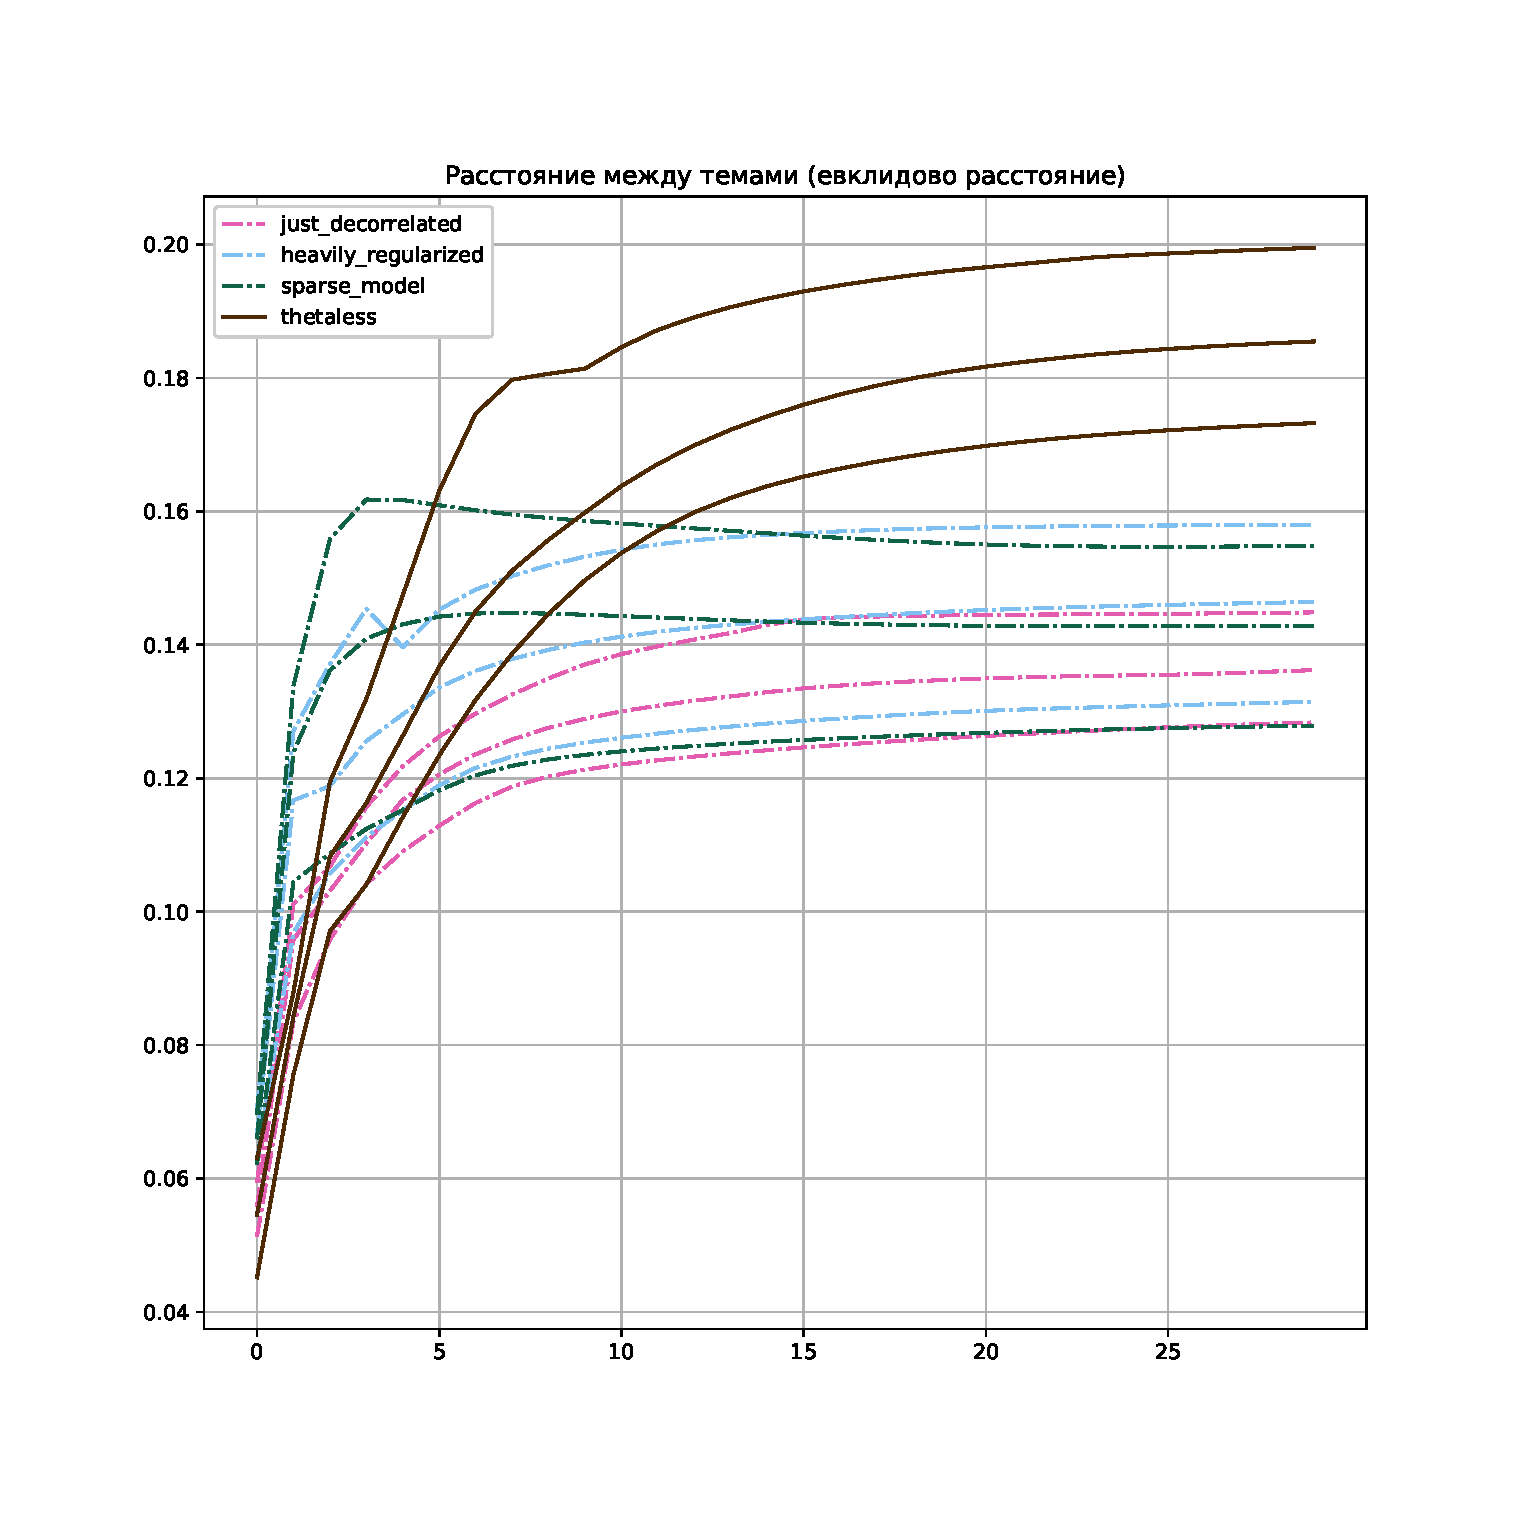
\includegraphics[width=55mm]{images/CH4_vs_regularized_diversity_euclidean_False.eps} &   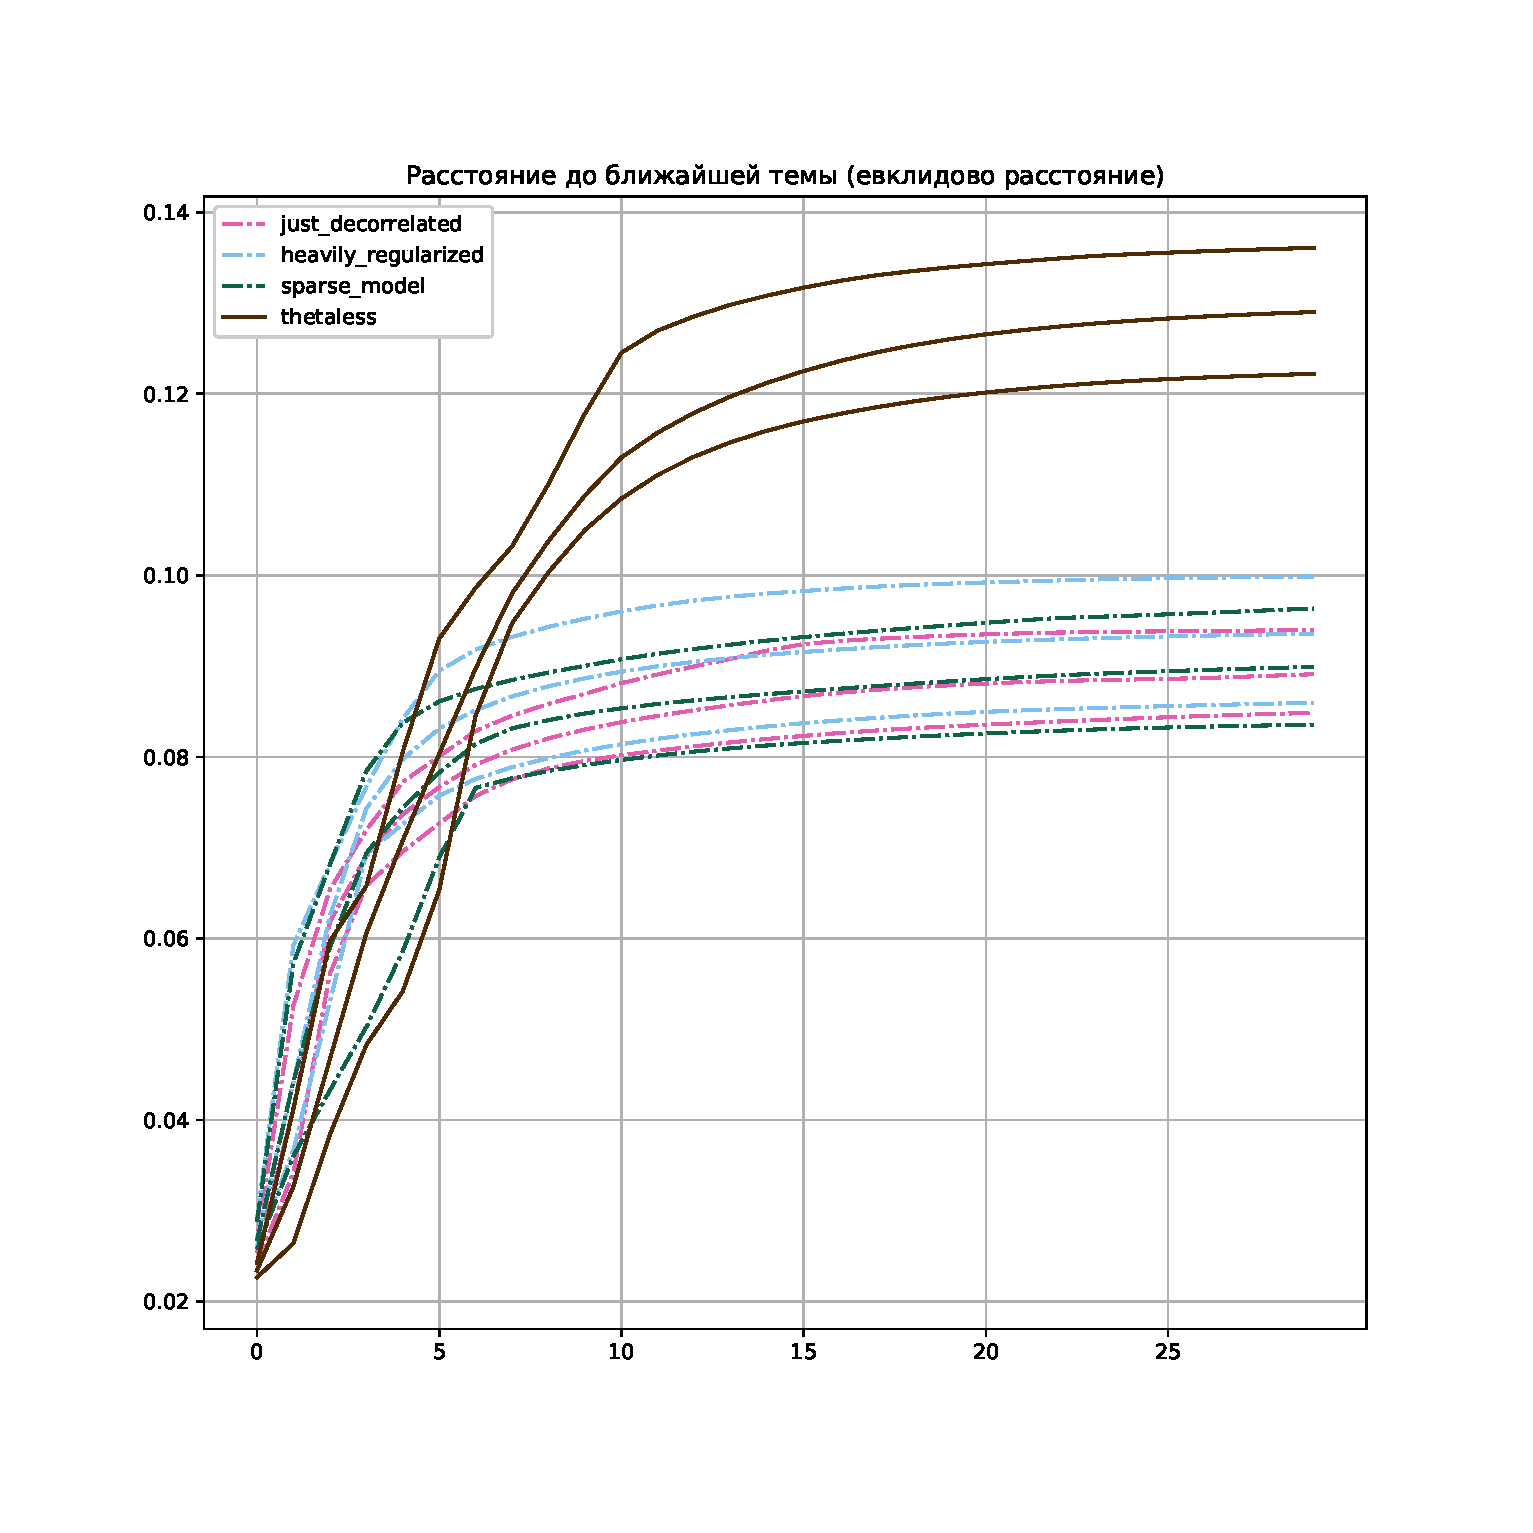
\includegraphics[width=55mm]{images/CH4_vs_regularized_diversity_euclidean_True.eps} & 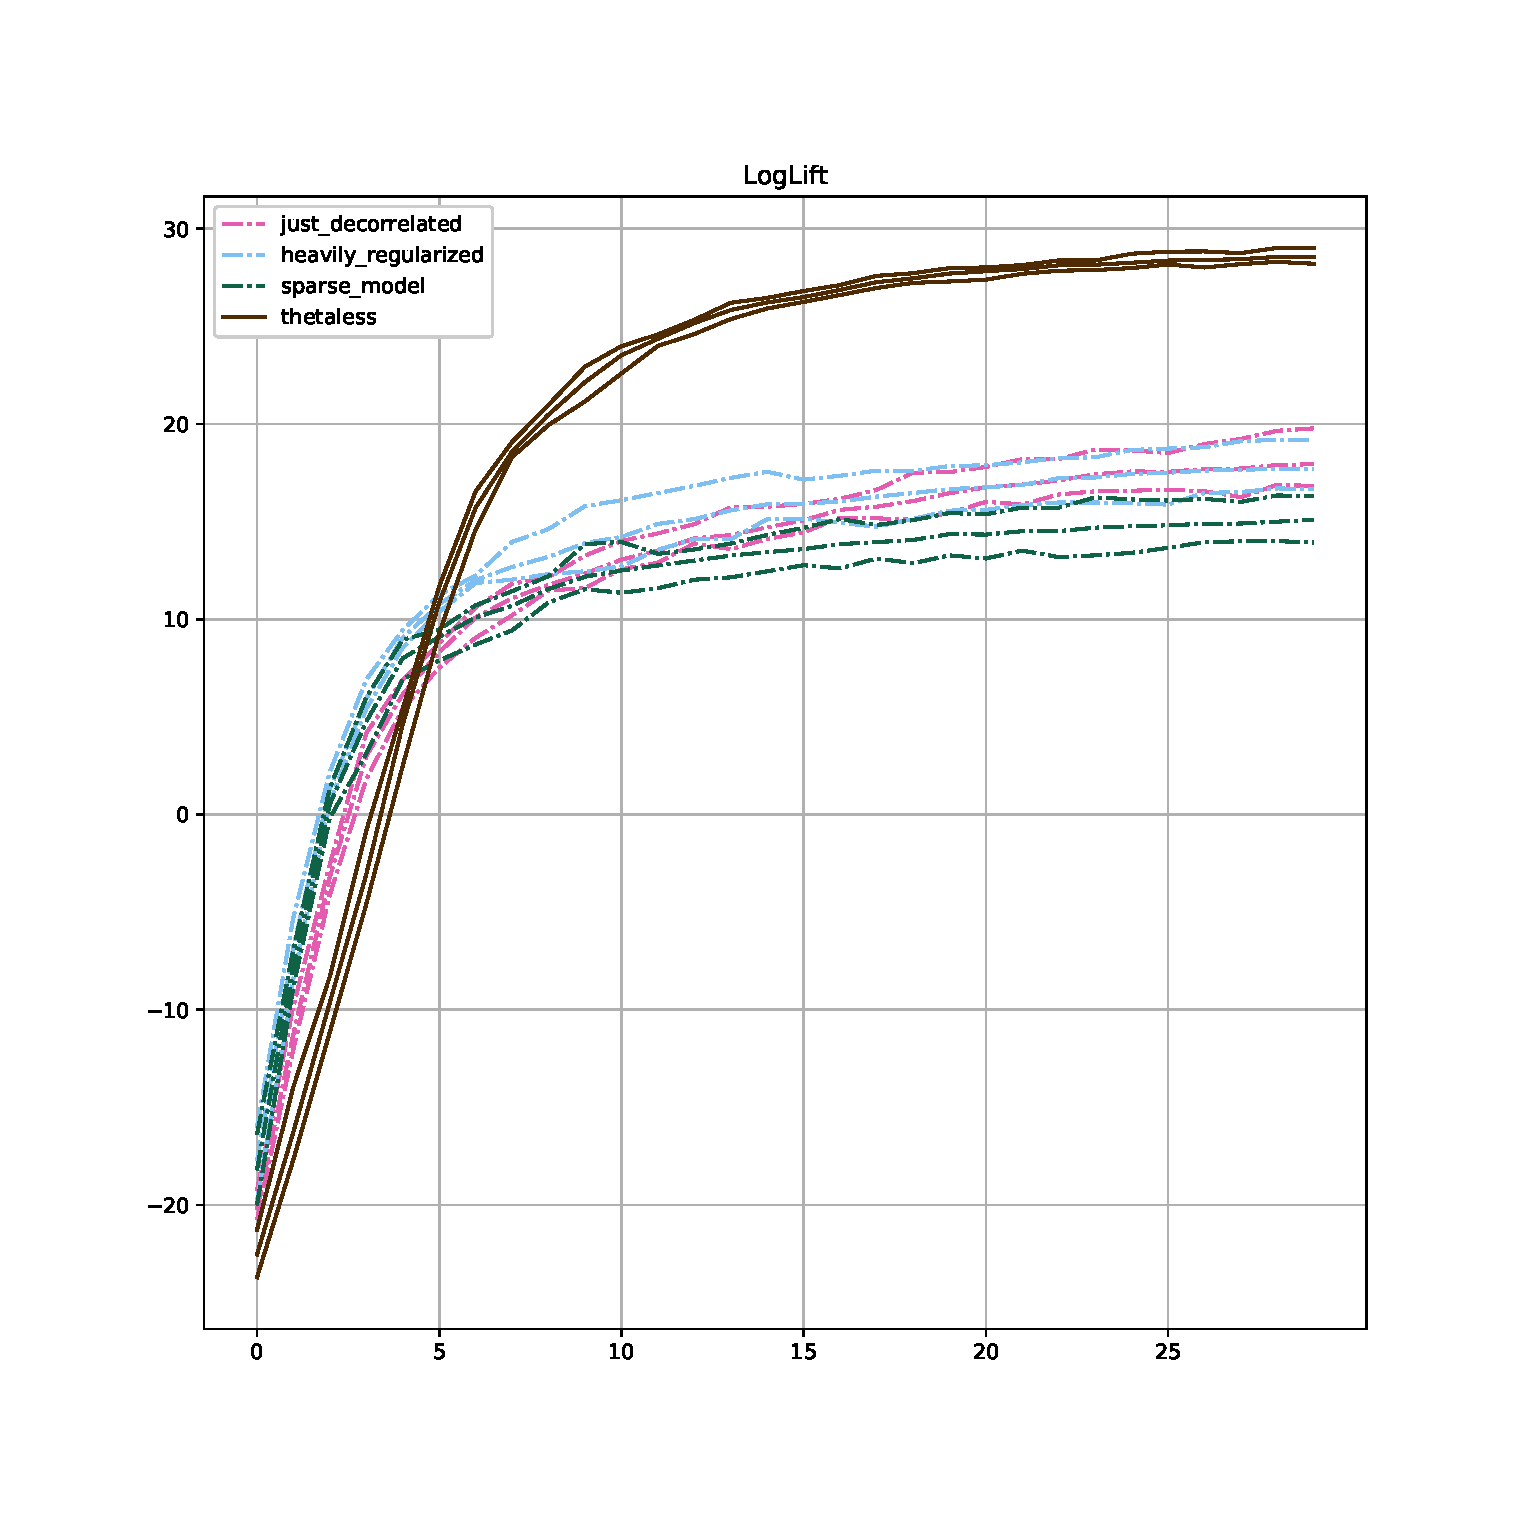
\includegraphics[width=55mm]{images/CH4_vs_regularized_loglift30.eps} \\
 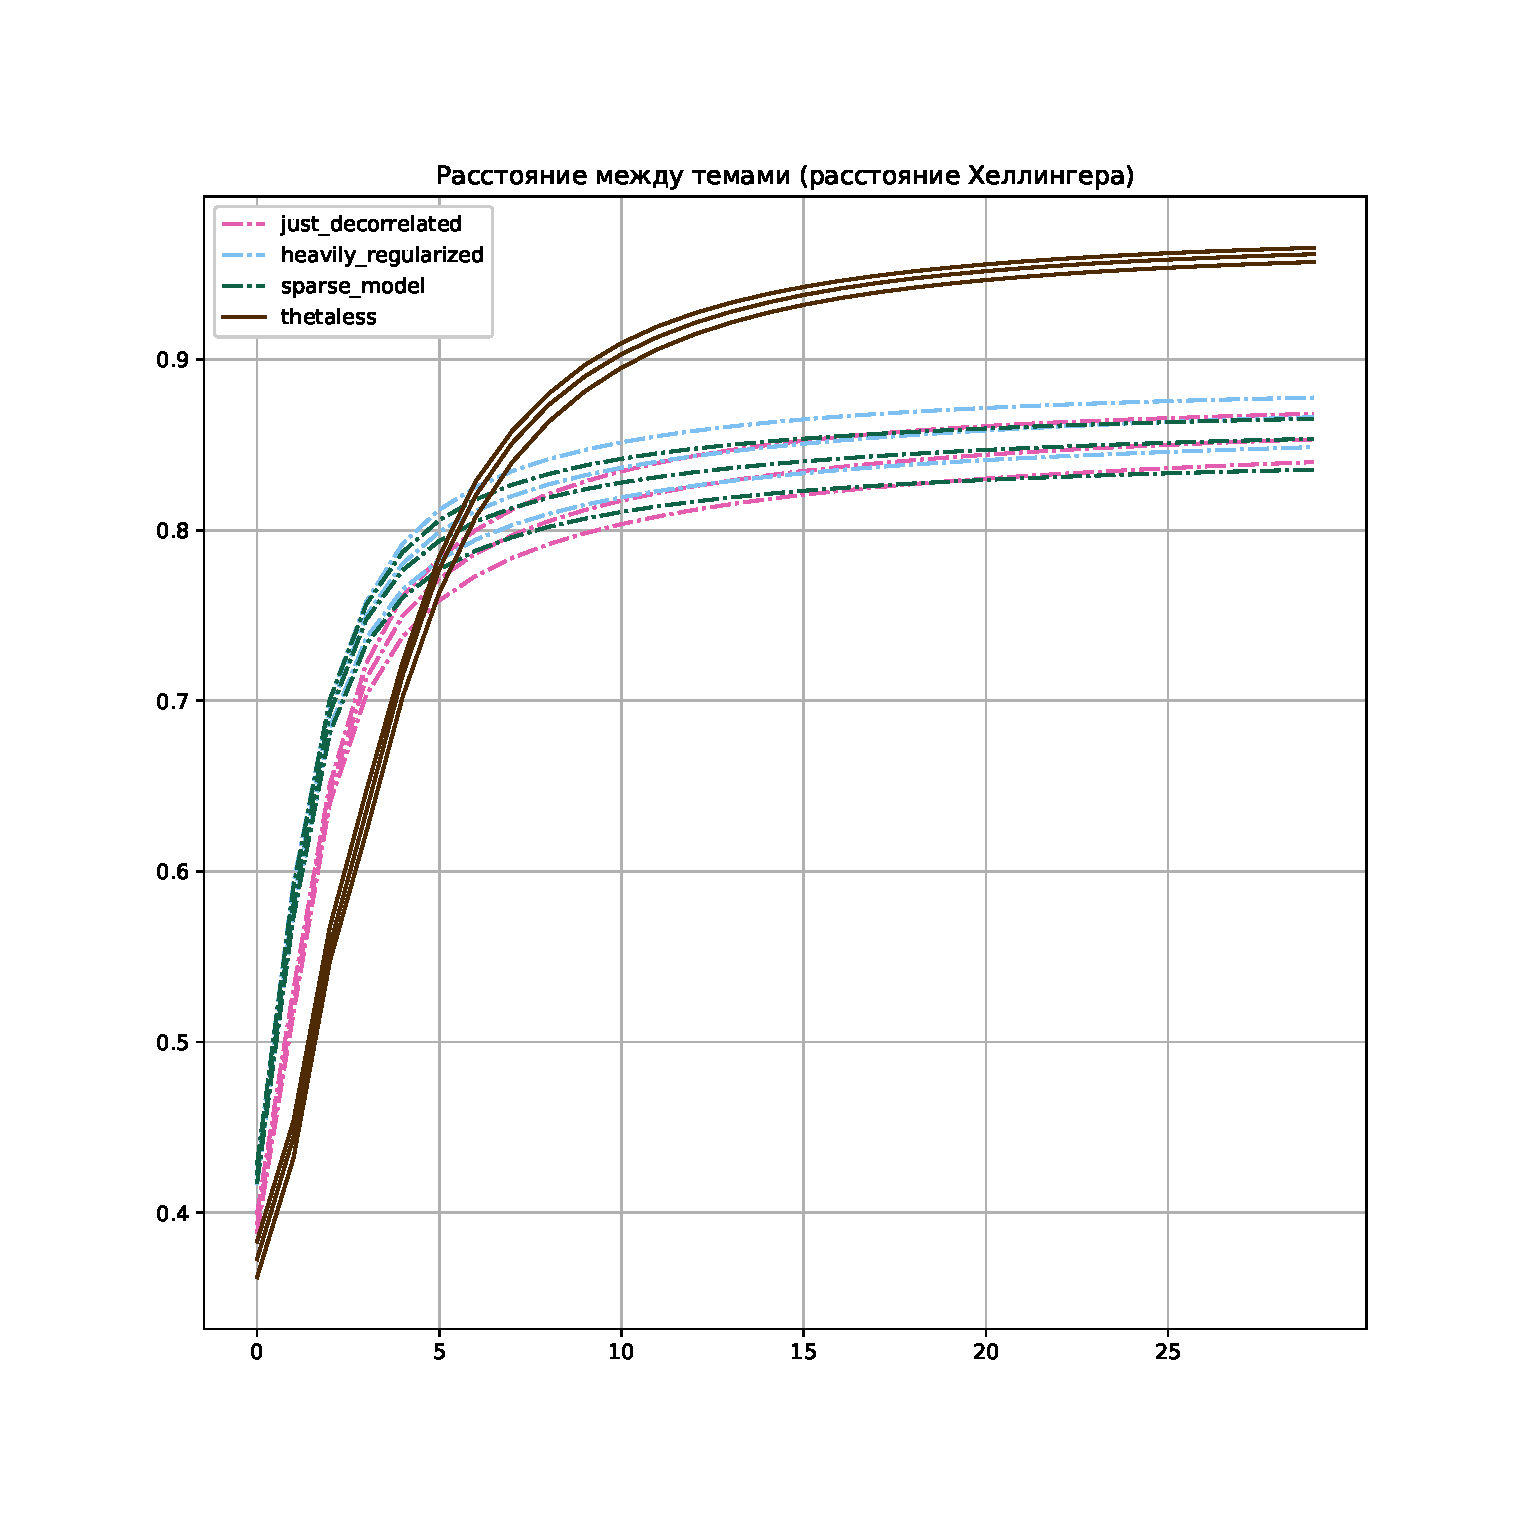
\includegraphics[width=55mm]{images/CH4_vs_regularized_diversity_hellinger_False.eps} &   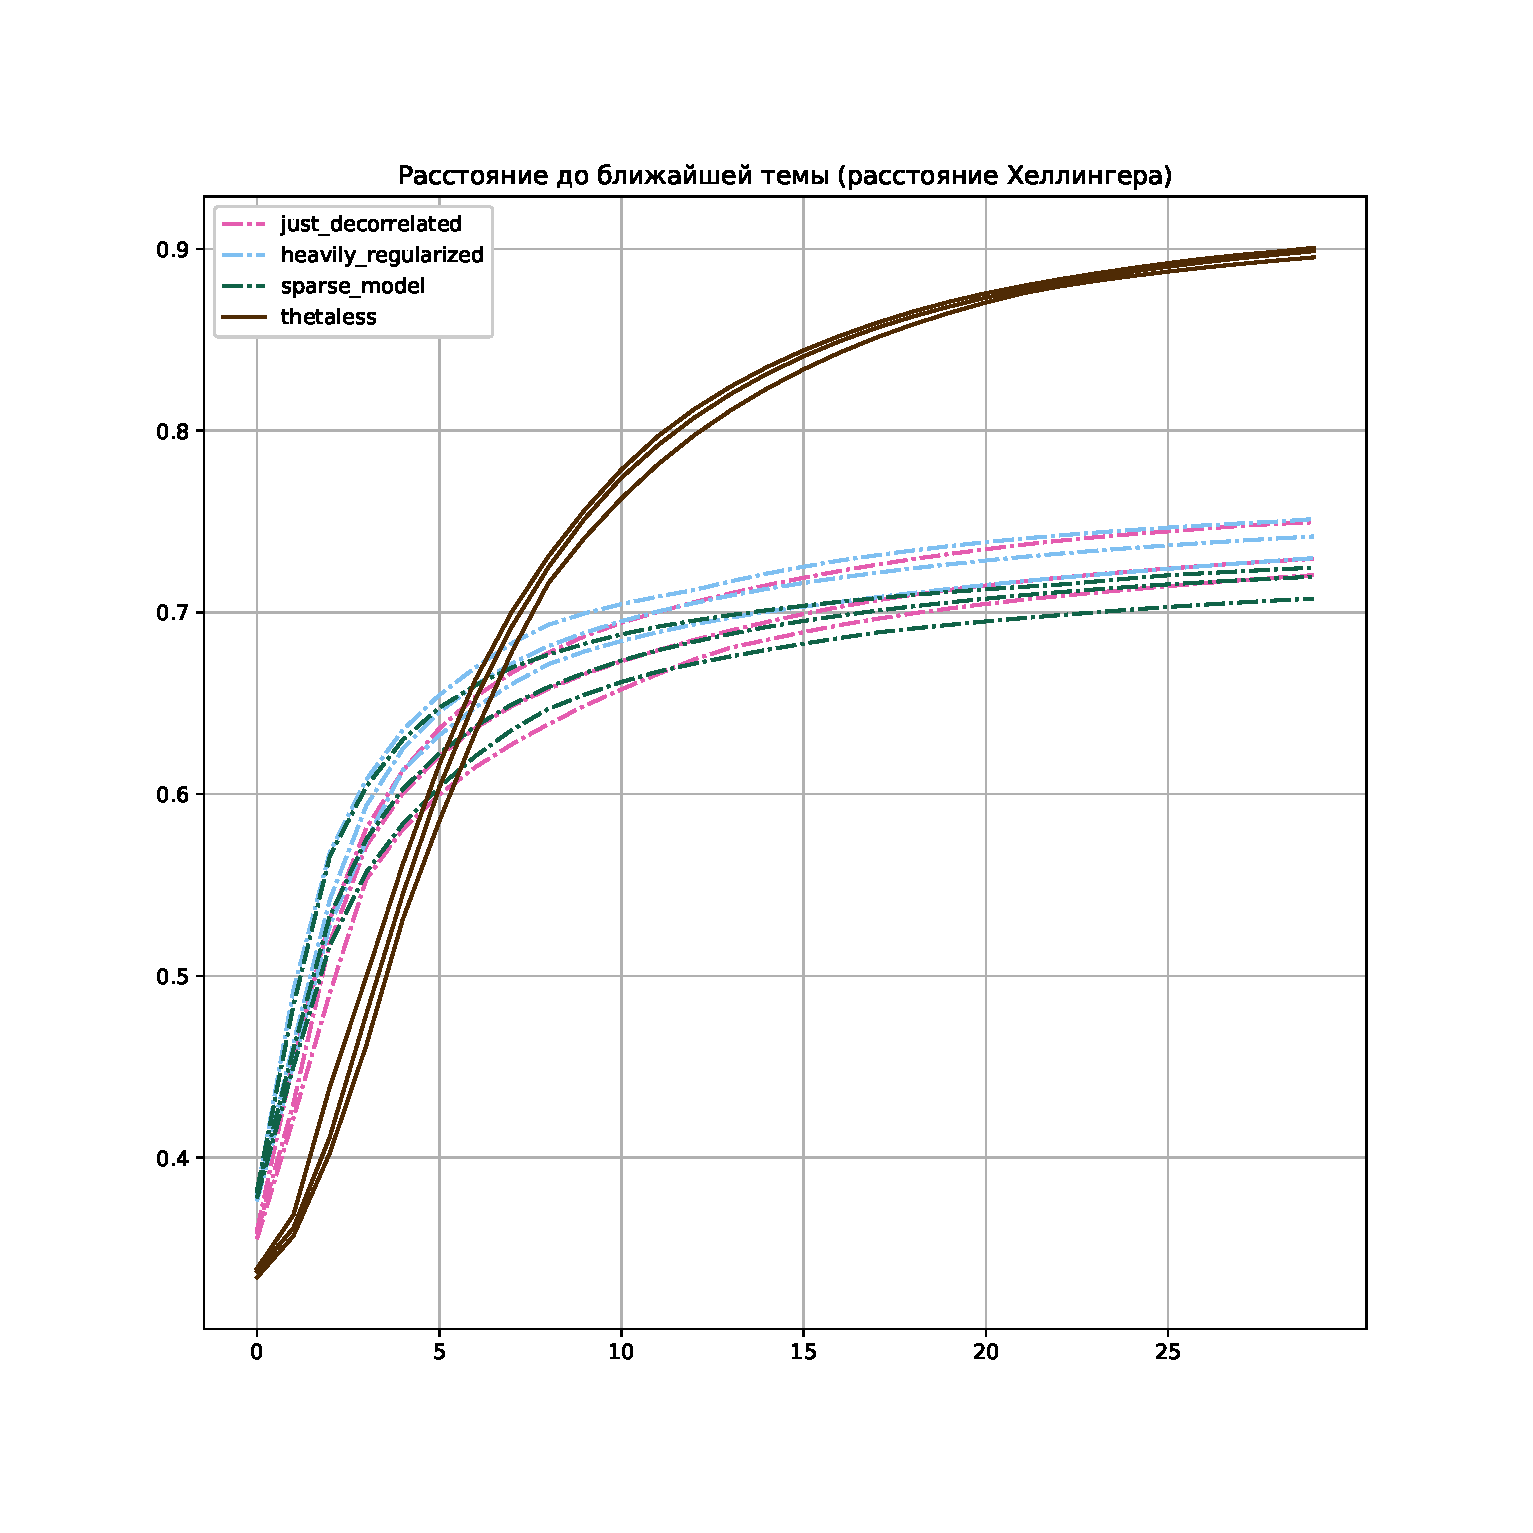
\includegraphics[width=55mm]{images/CH4_vs_regularized_diversity_hellinger_True.eps} & 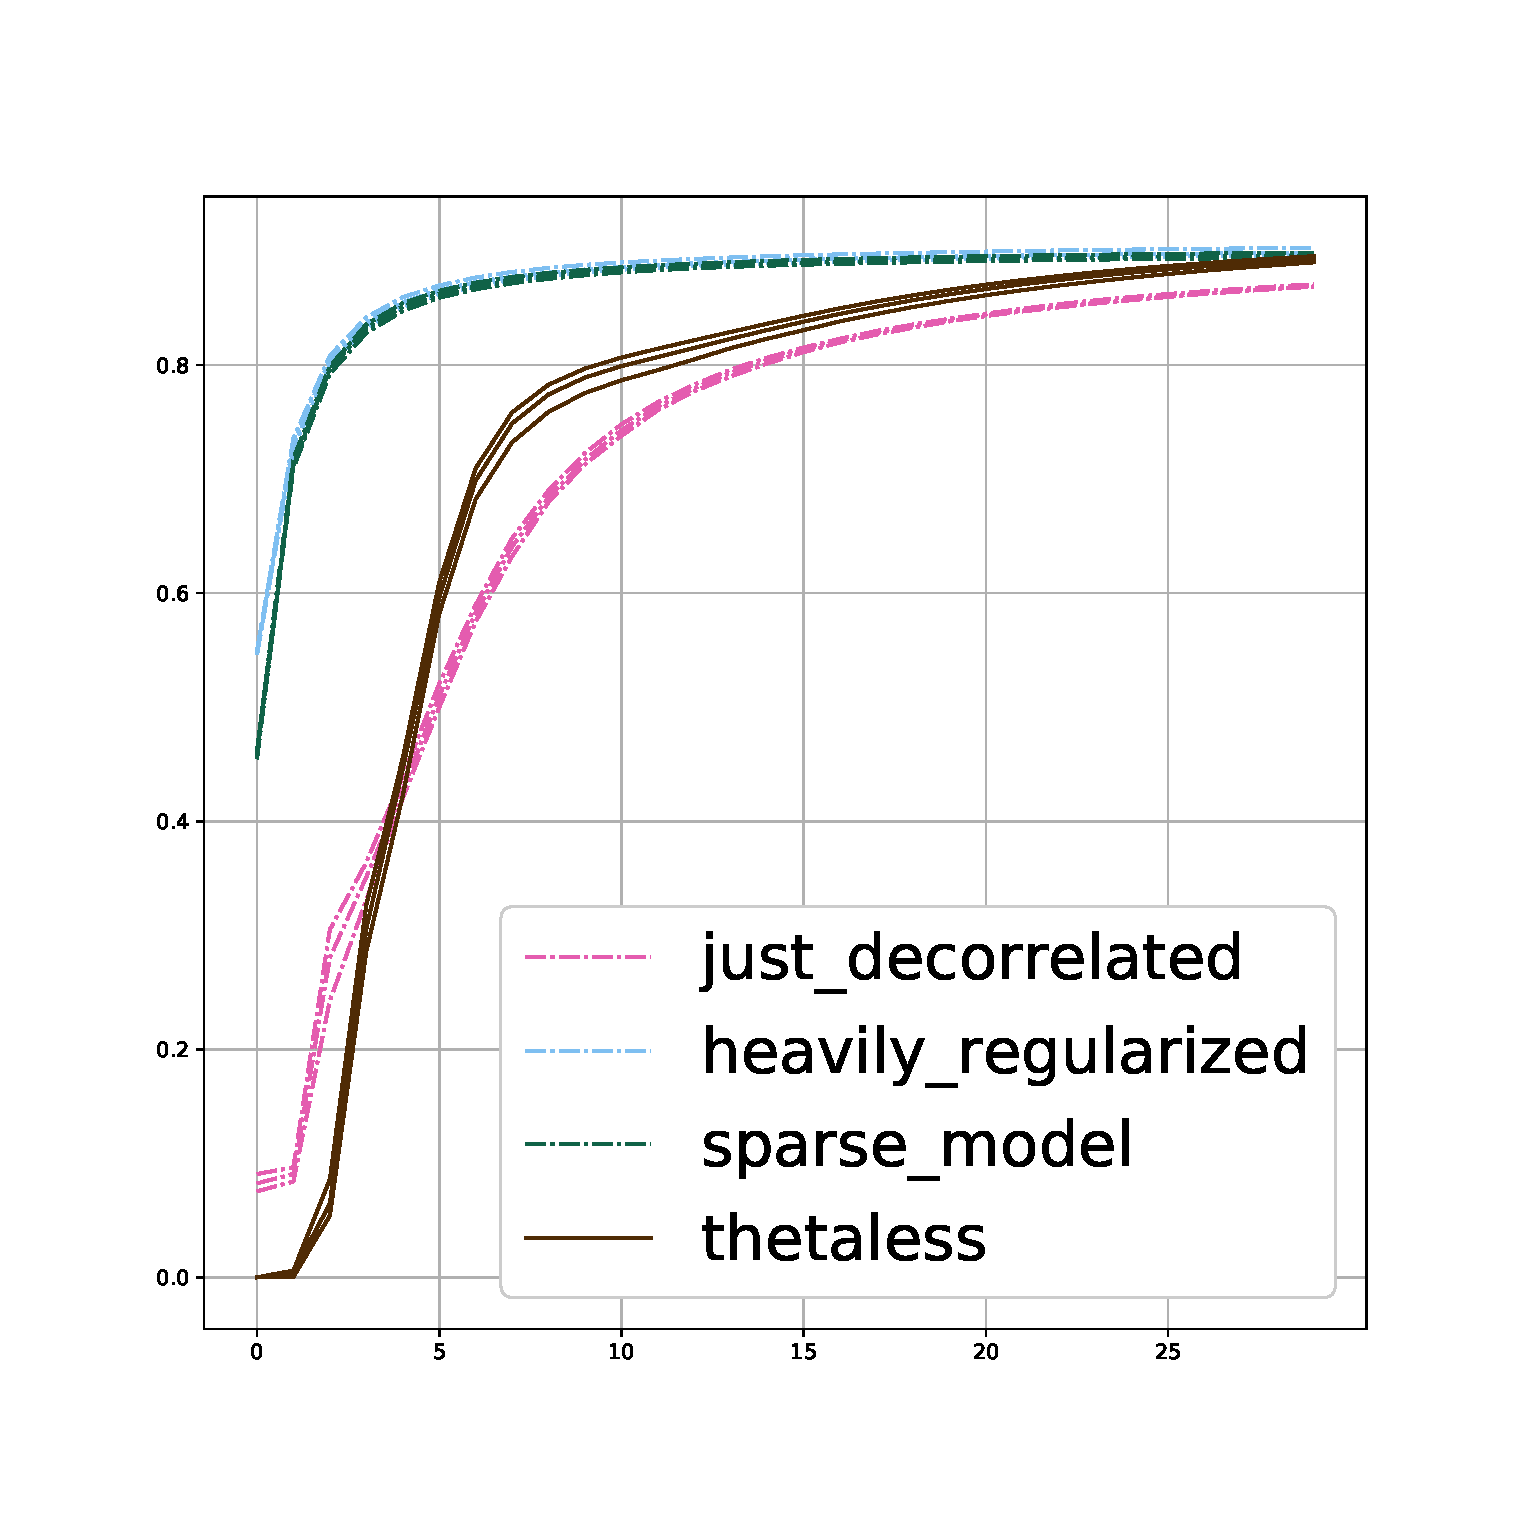
\includegraphics[width=55mm]{images/CH4_vs_regularized_SparsityPhiScore.eps} \\    
    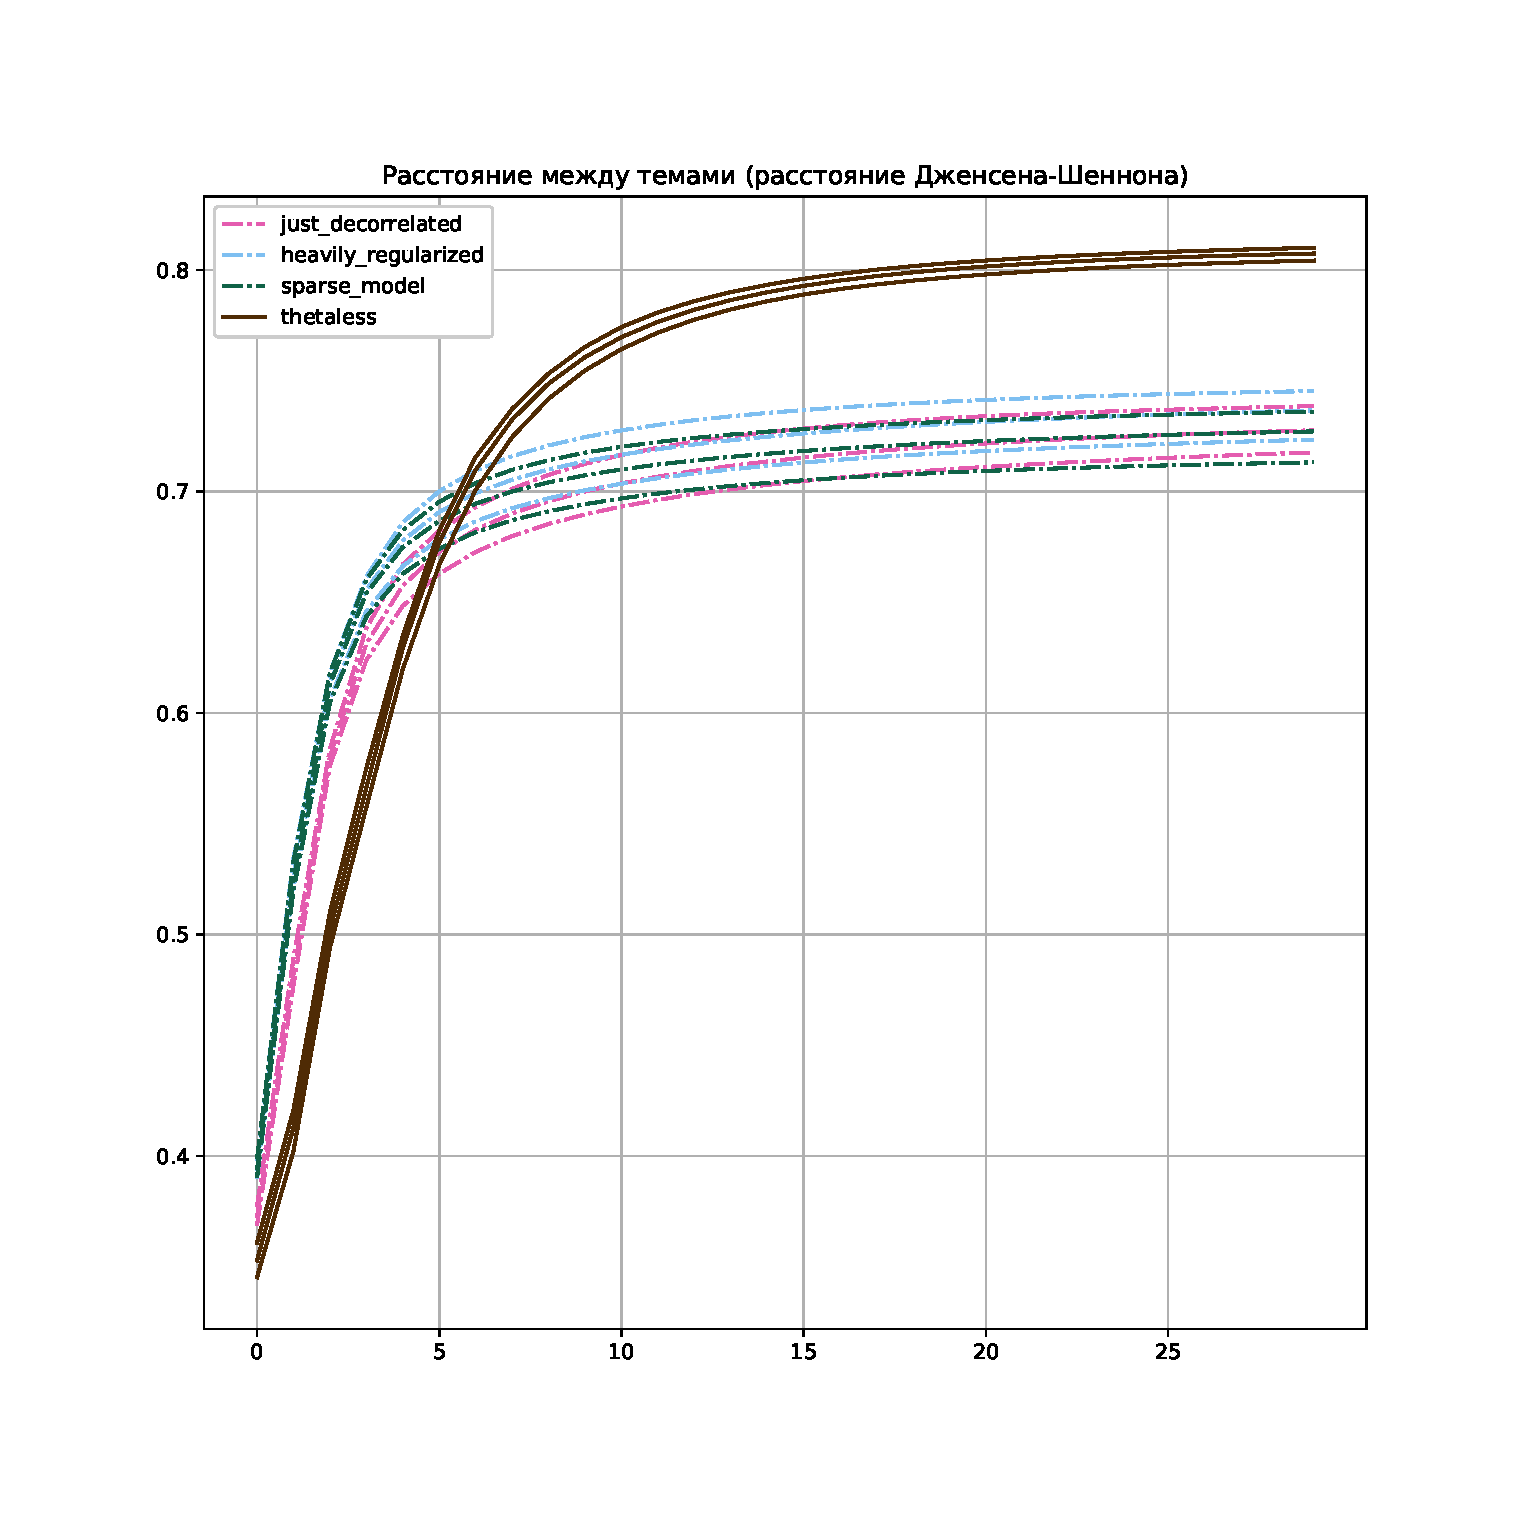
\includegraphics[width=55mm]{images/CH4_vs_regularized_diversity_jensenshannon_False.eps} &   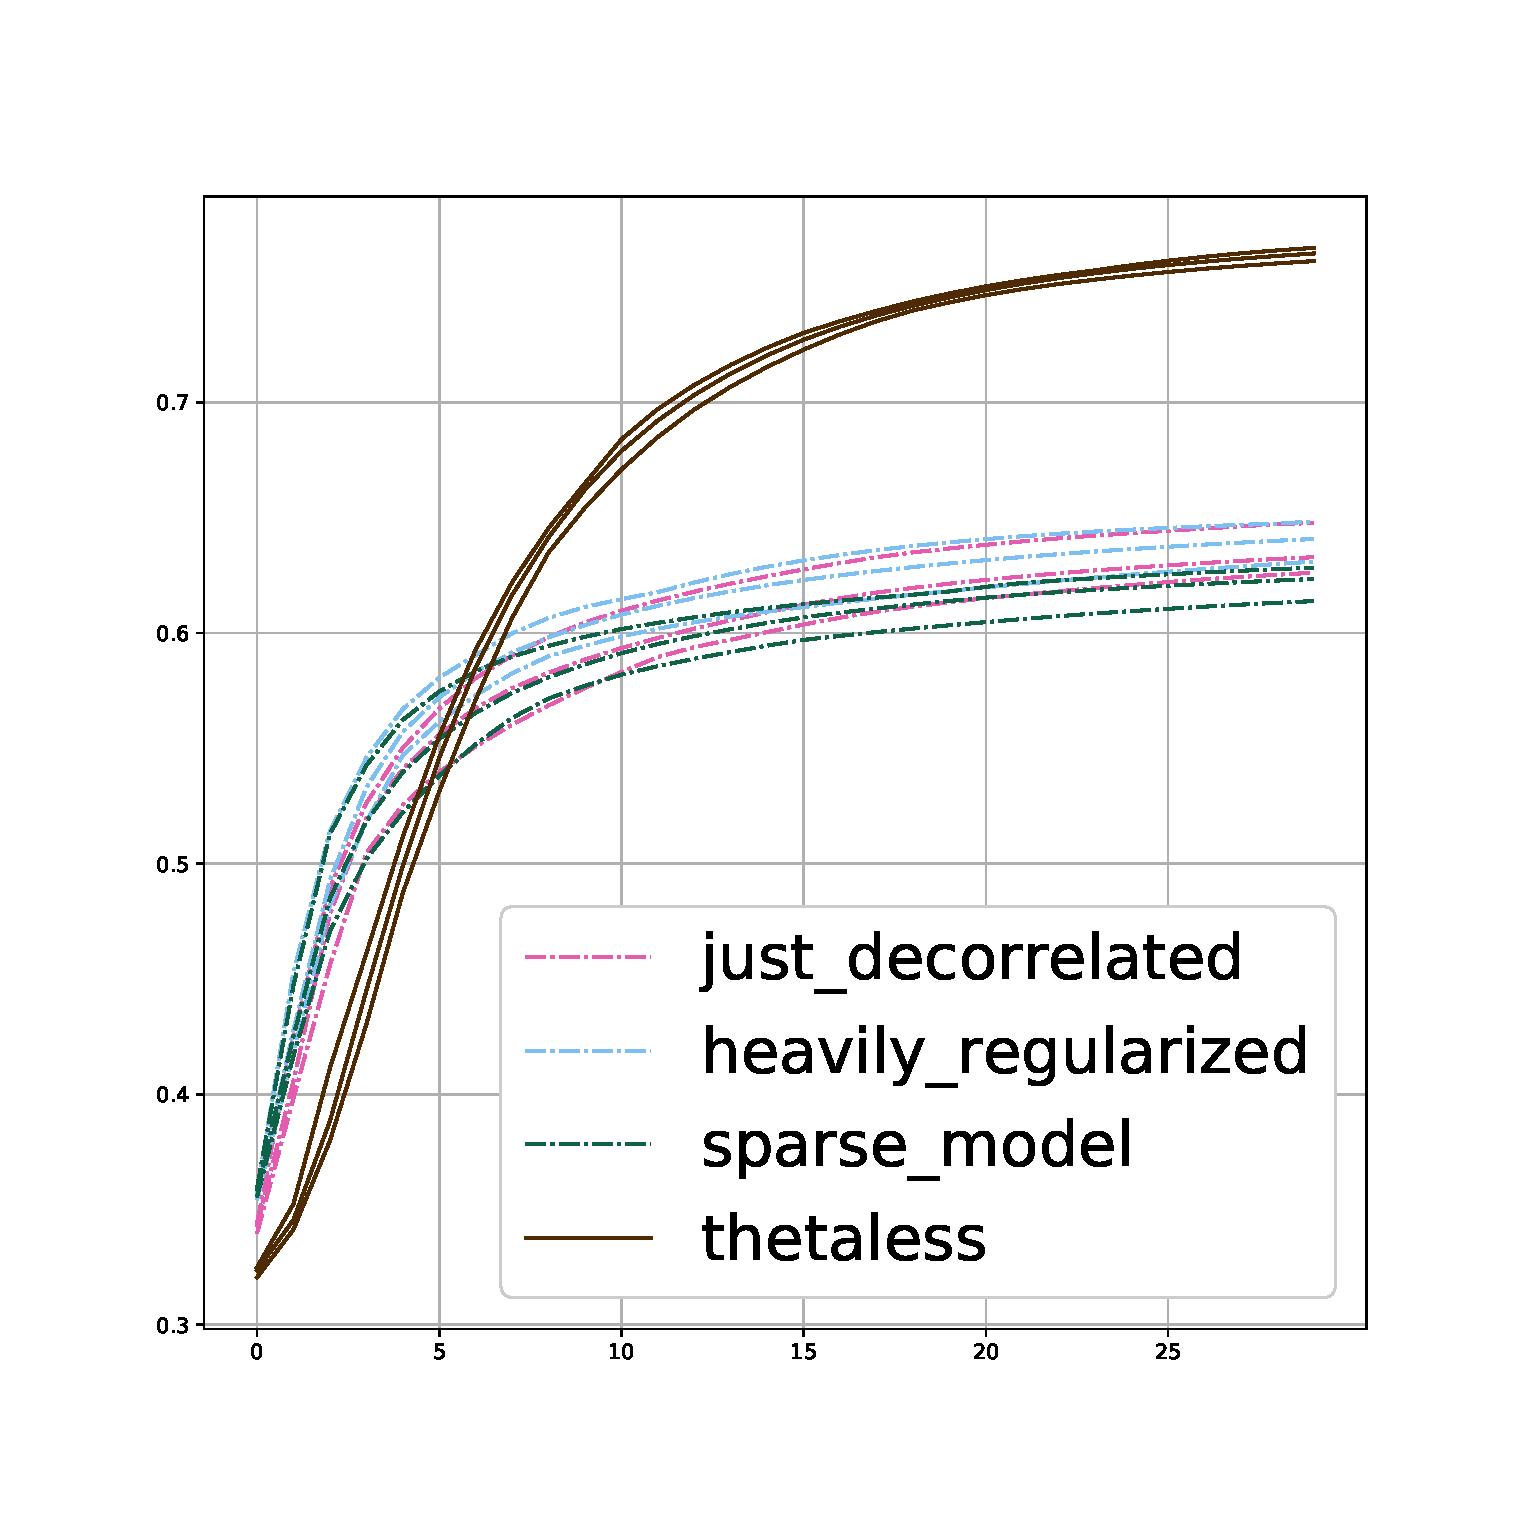
\includegraphics[width=55mm]{images/CH4_vs_regularized_diversity_jensenshannon_True.eps} & 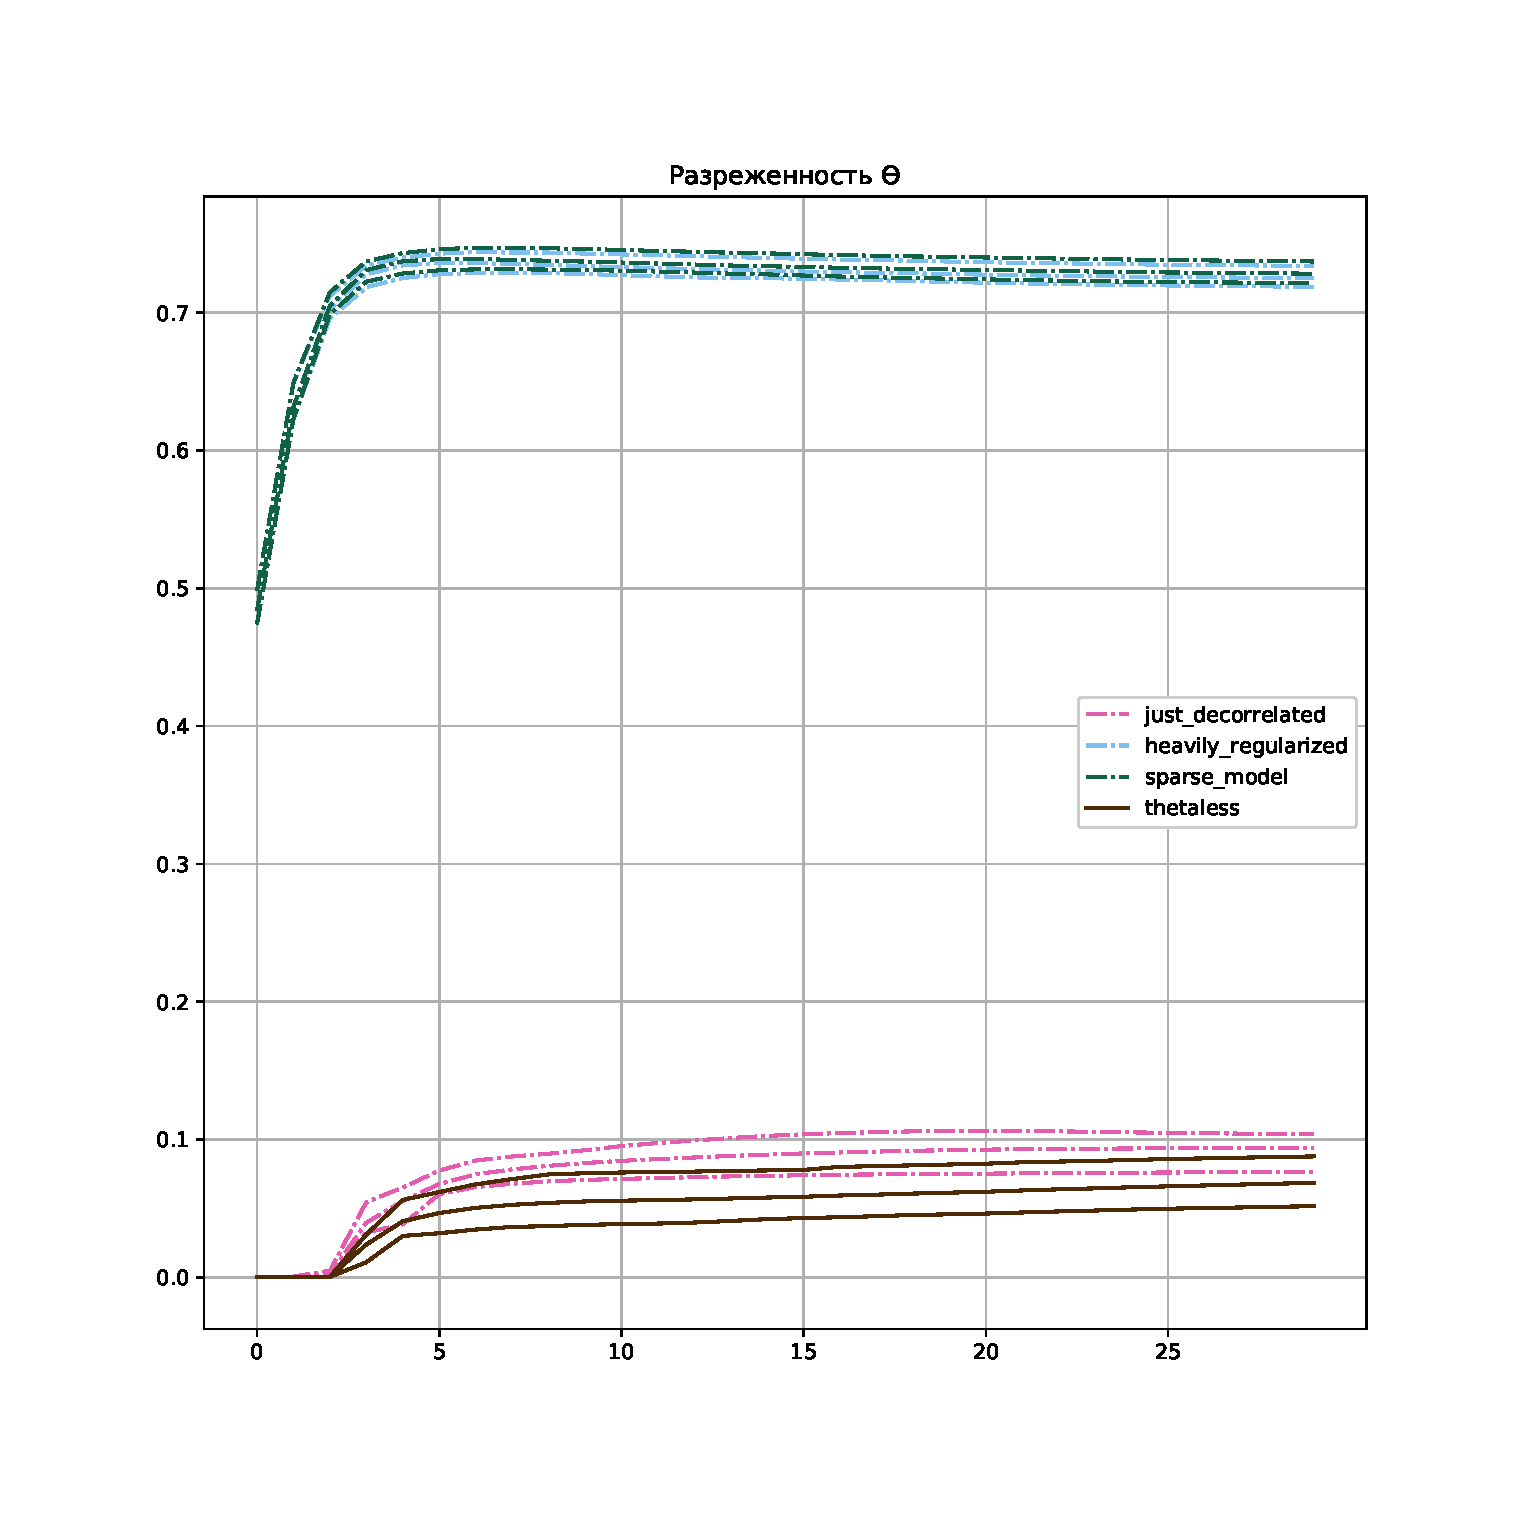
\includegraphics[width=55mm]{images/CH4_vs_regularized_SparsityThetaScore.eps} \\
\end{tabular}
    \caption{Графики зависимости различных критериев качества тематических моделей для пяти моделей (TARTM, PLSA, LDA с 3 видами приоров). Каждой модели соответствуют три линии: среднее значение, минимум и максимум (по пяти случайным перезапускам).}
\label{fig:ch4_vs_reg}
\end{figure}


\begin{figure}
\begin{tabular}{ccc}
    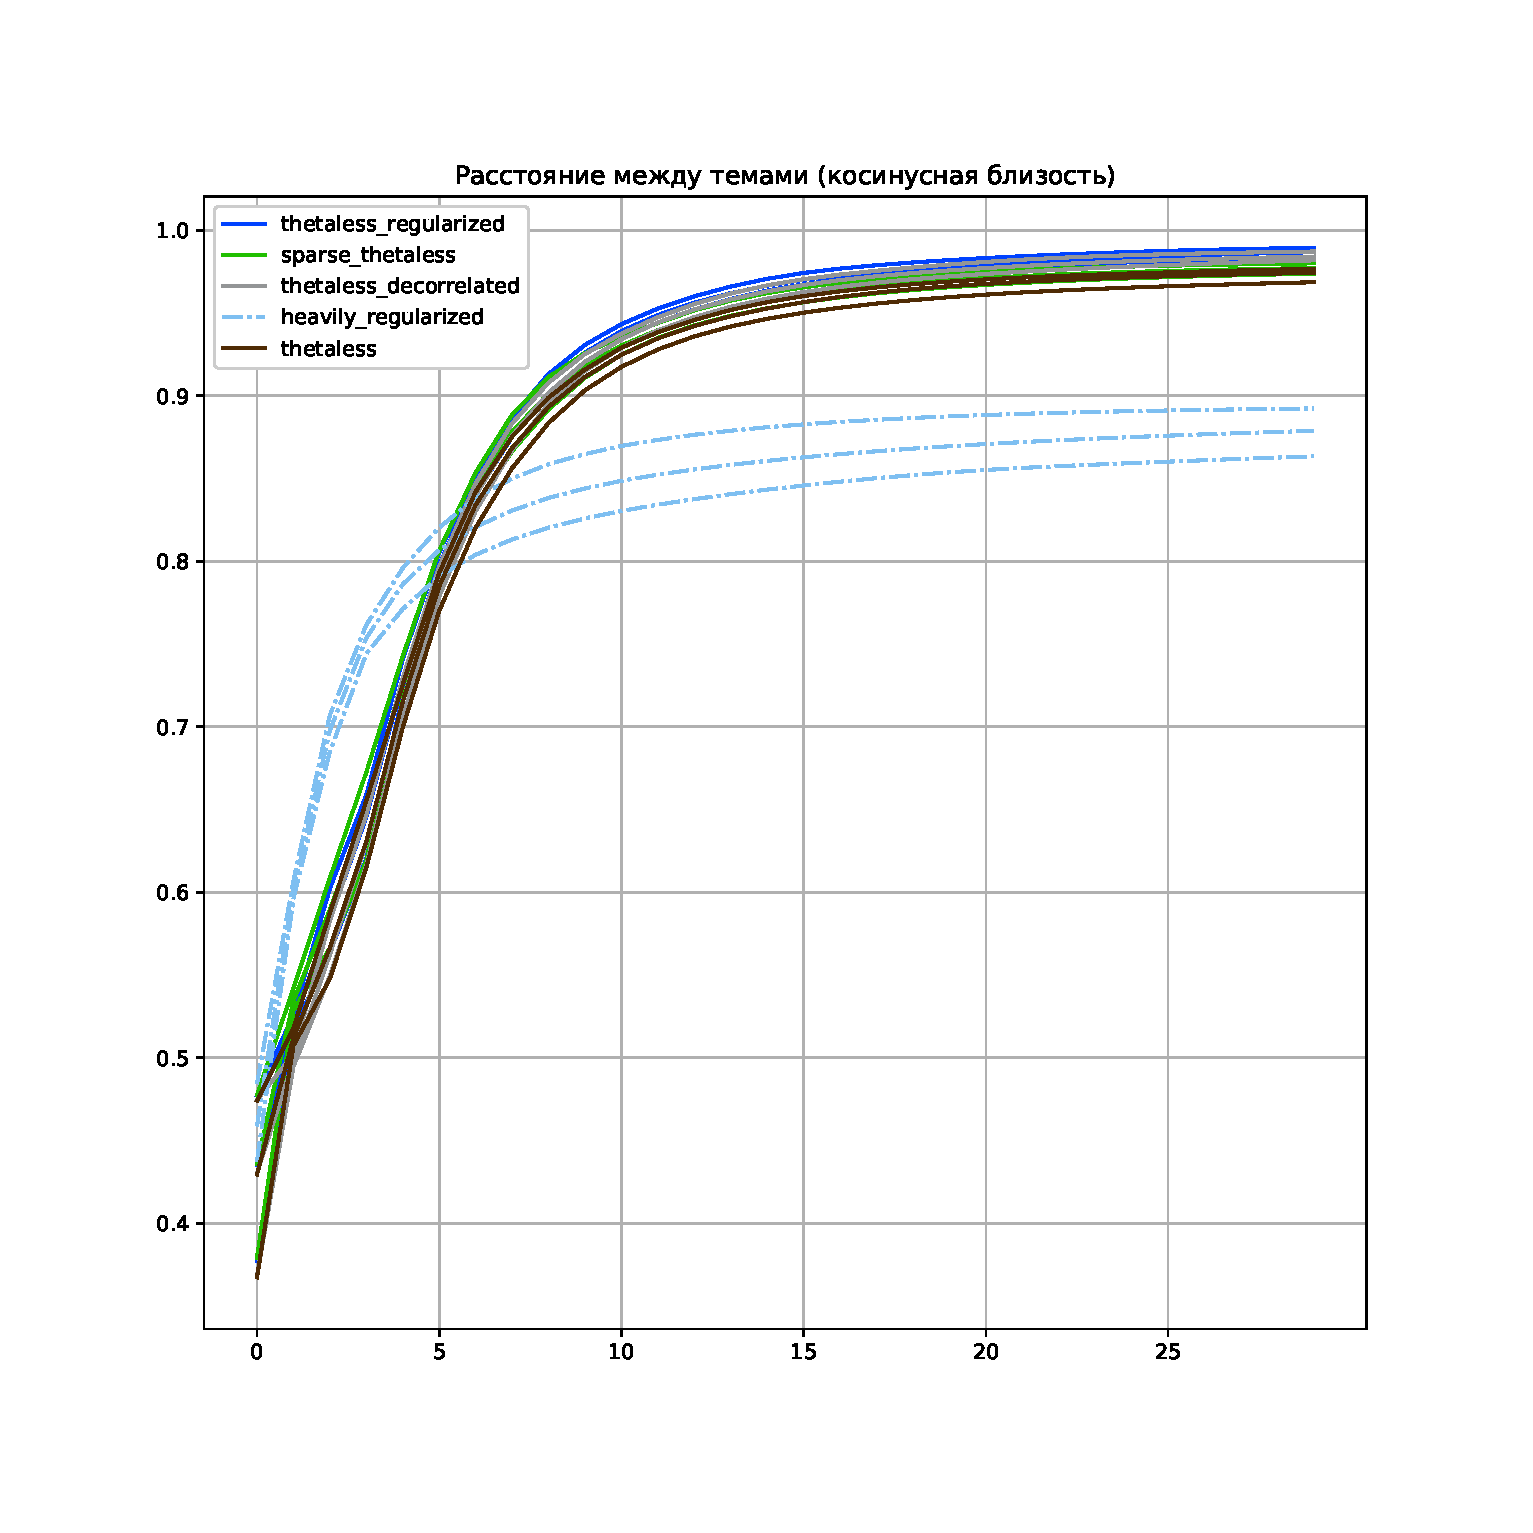
\includegraphics[width=55mm]{images/CH4_improved_diversity_cosine_False.eps} &   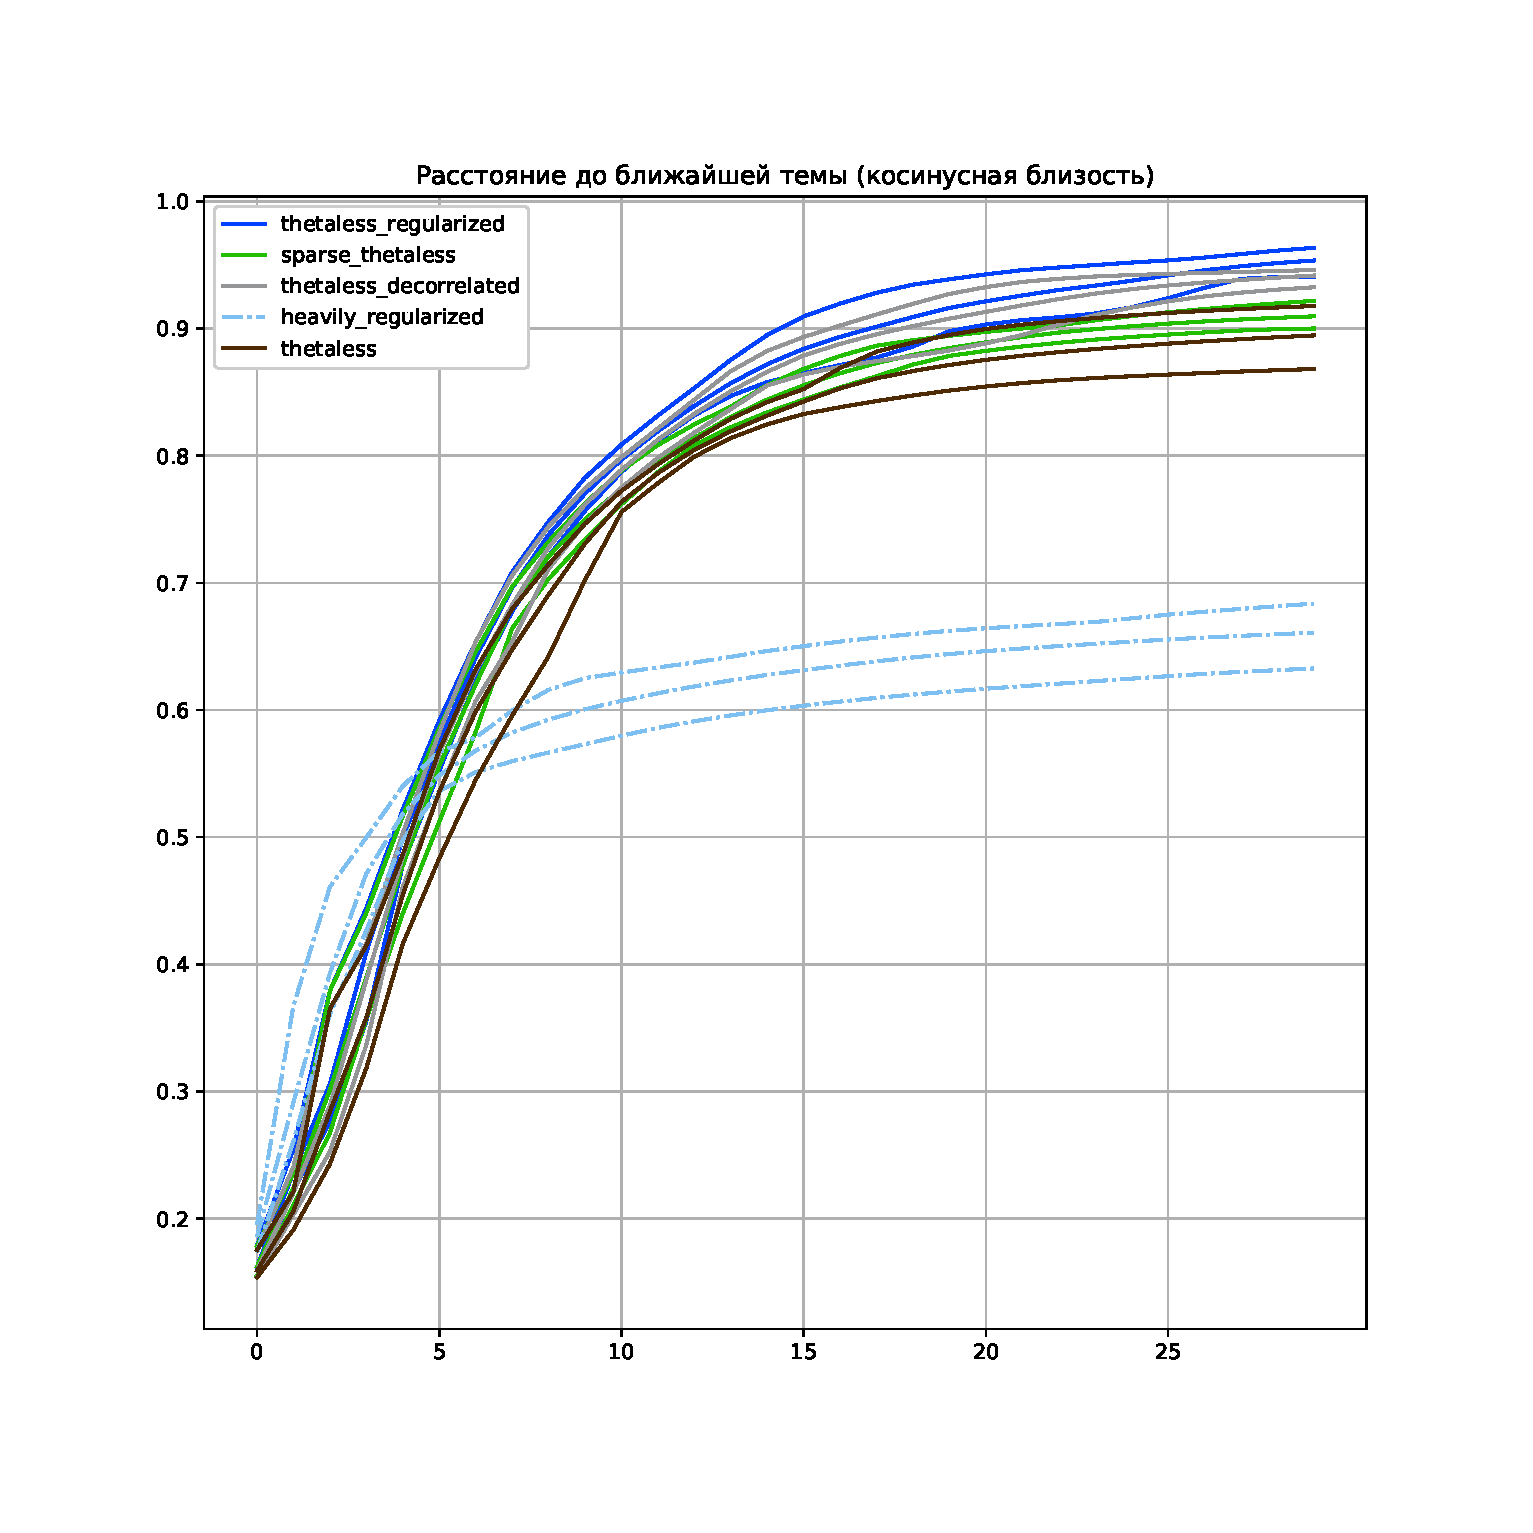
\includegraphics[width=55mm]{images/CH4_improved_diversity_cosine_True.eps} & 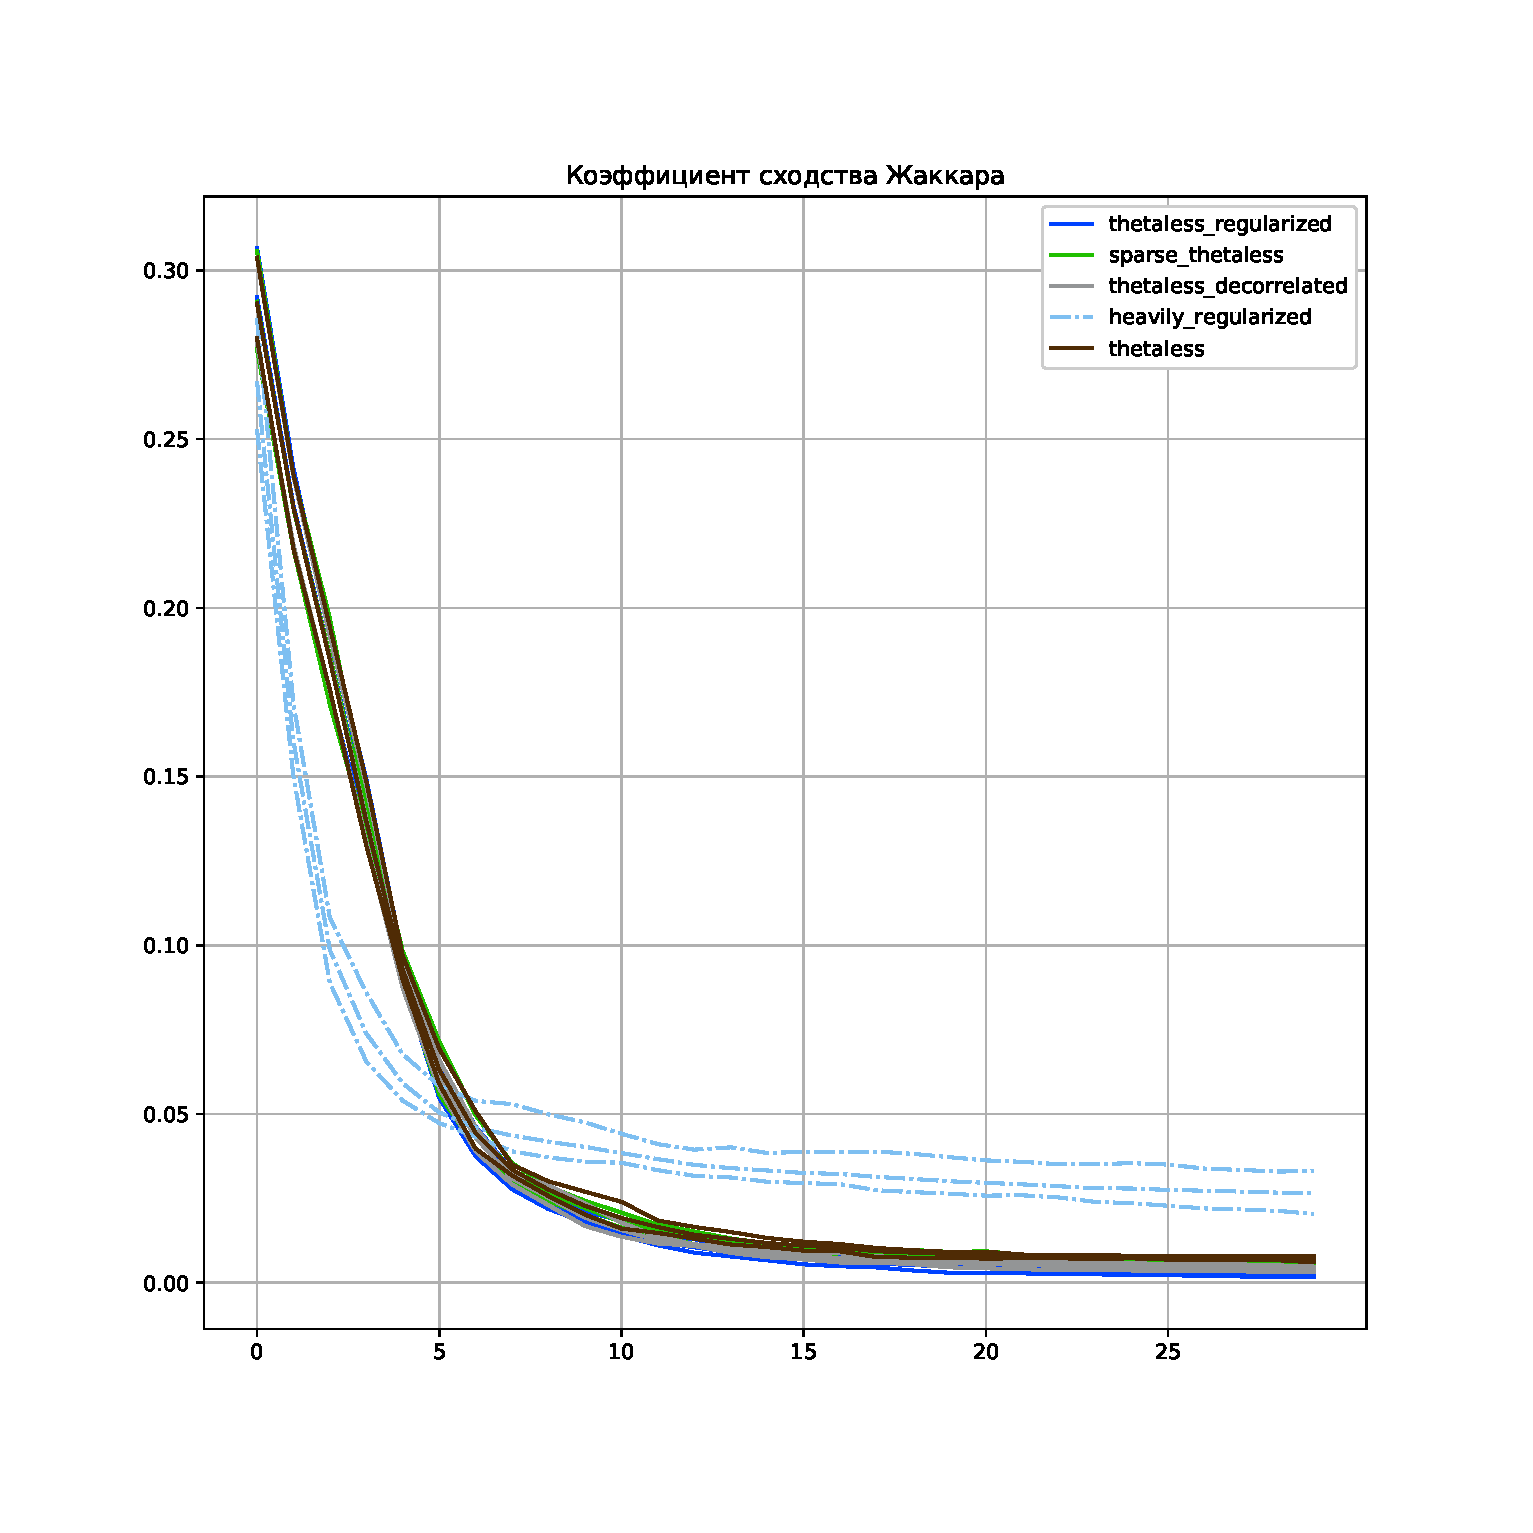
\includegraphics[width=55mm]{images/CH4_improved_jaccard_sim_30.eps} \\
    
    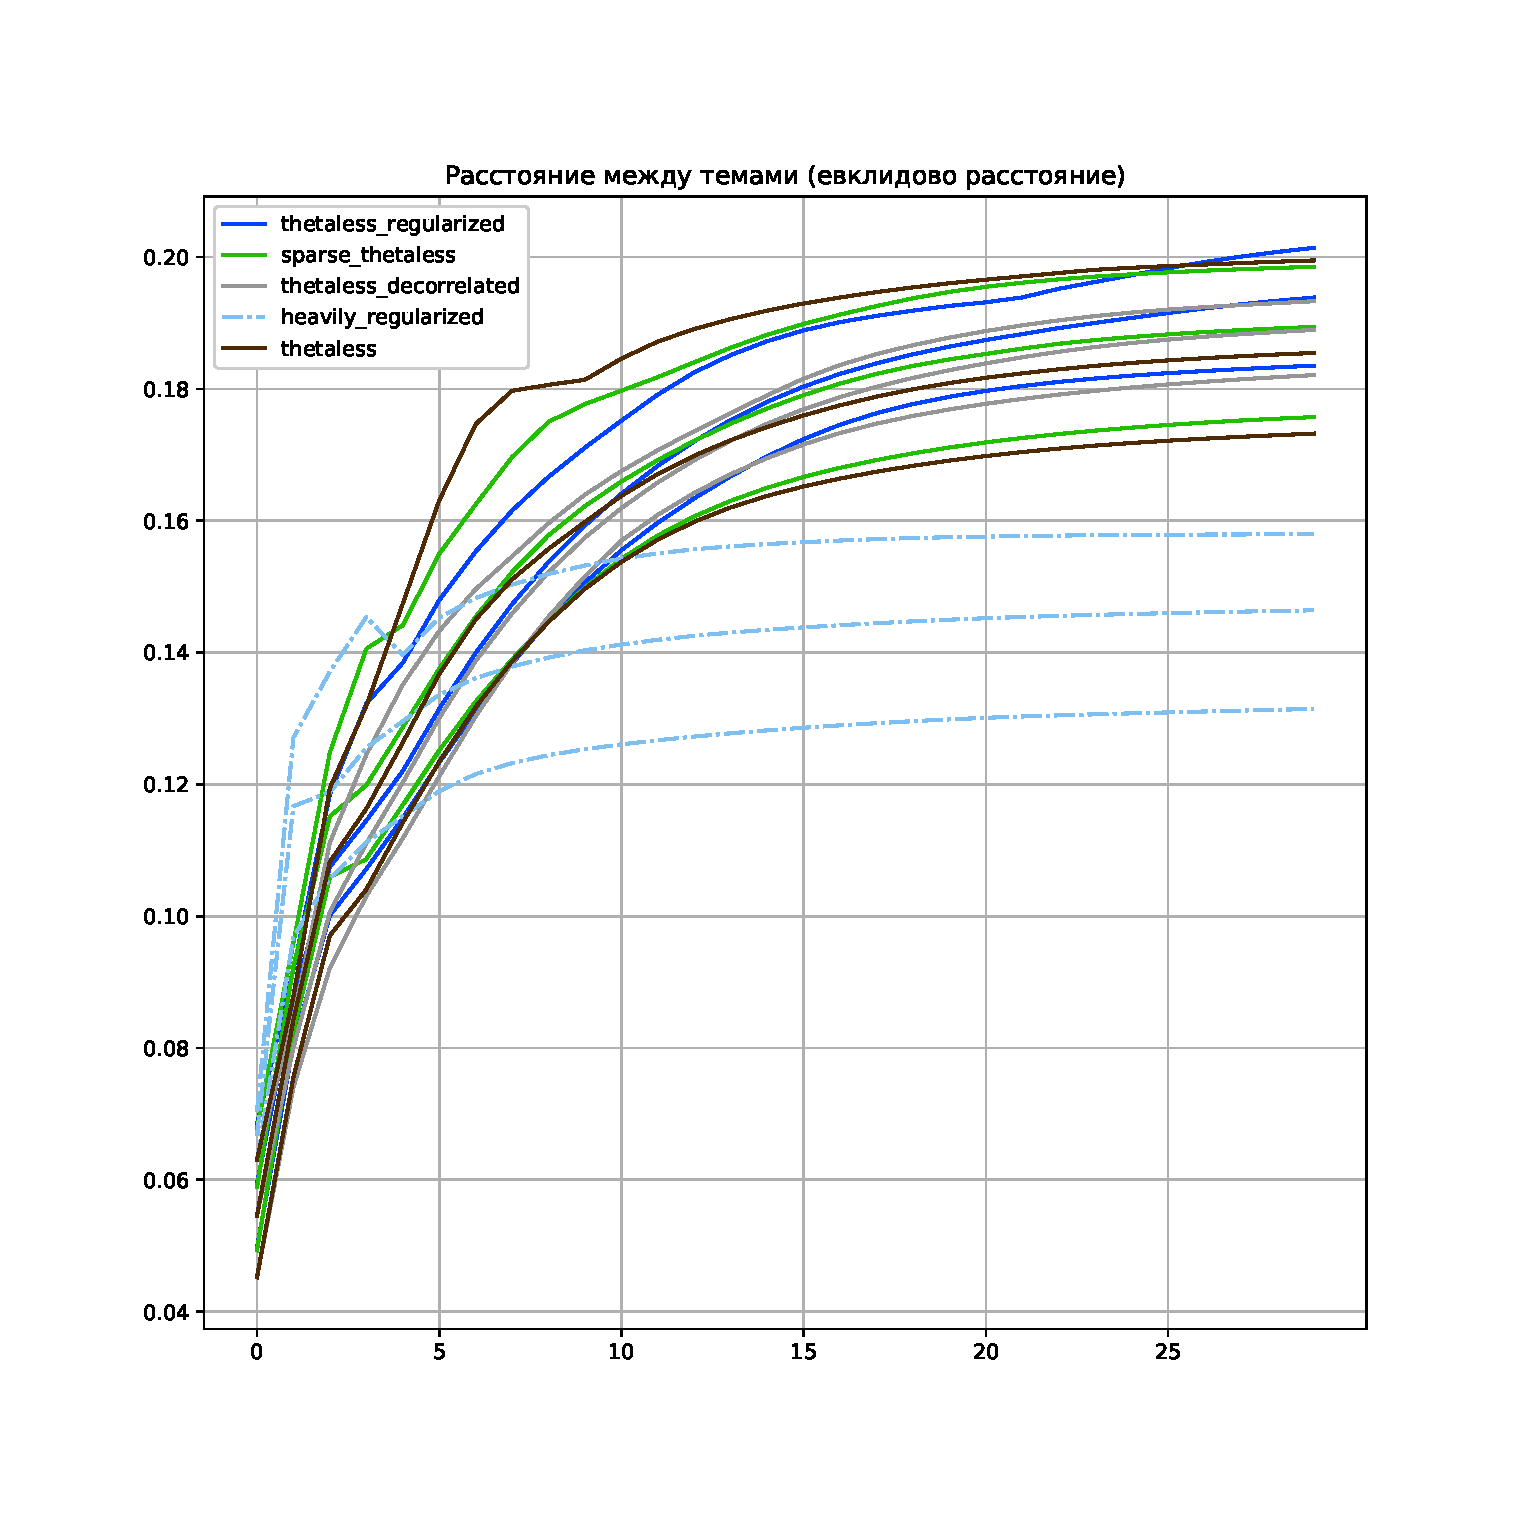
\includegraphics[width=55mm]{images/CH4_improved_diversity_euclidean_False.eps} &   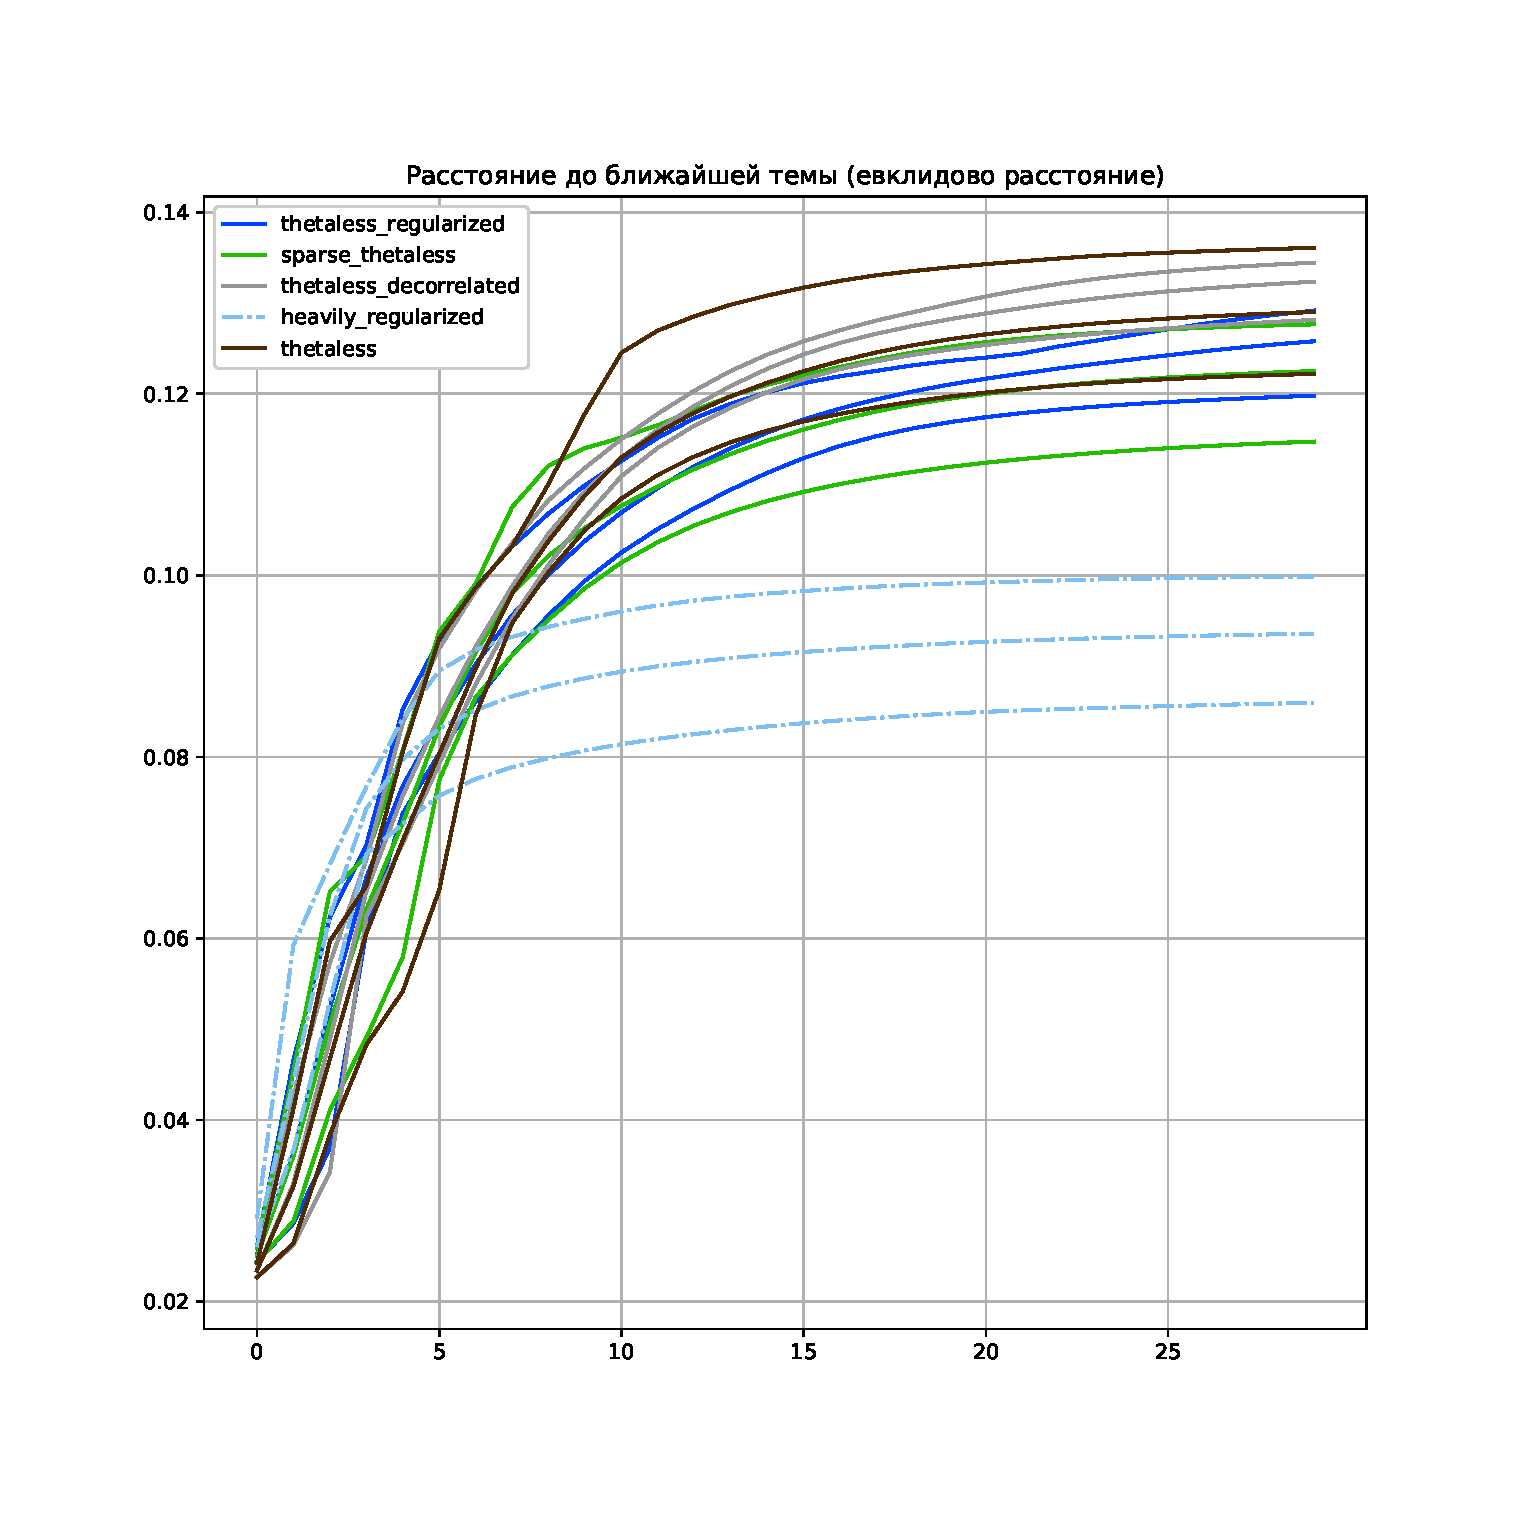
\includegraphics[width=55mm]{images/CH4_improved_diversity_euclidean_True.eps} & 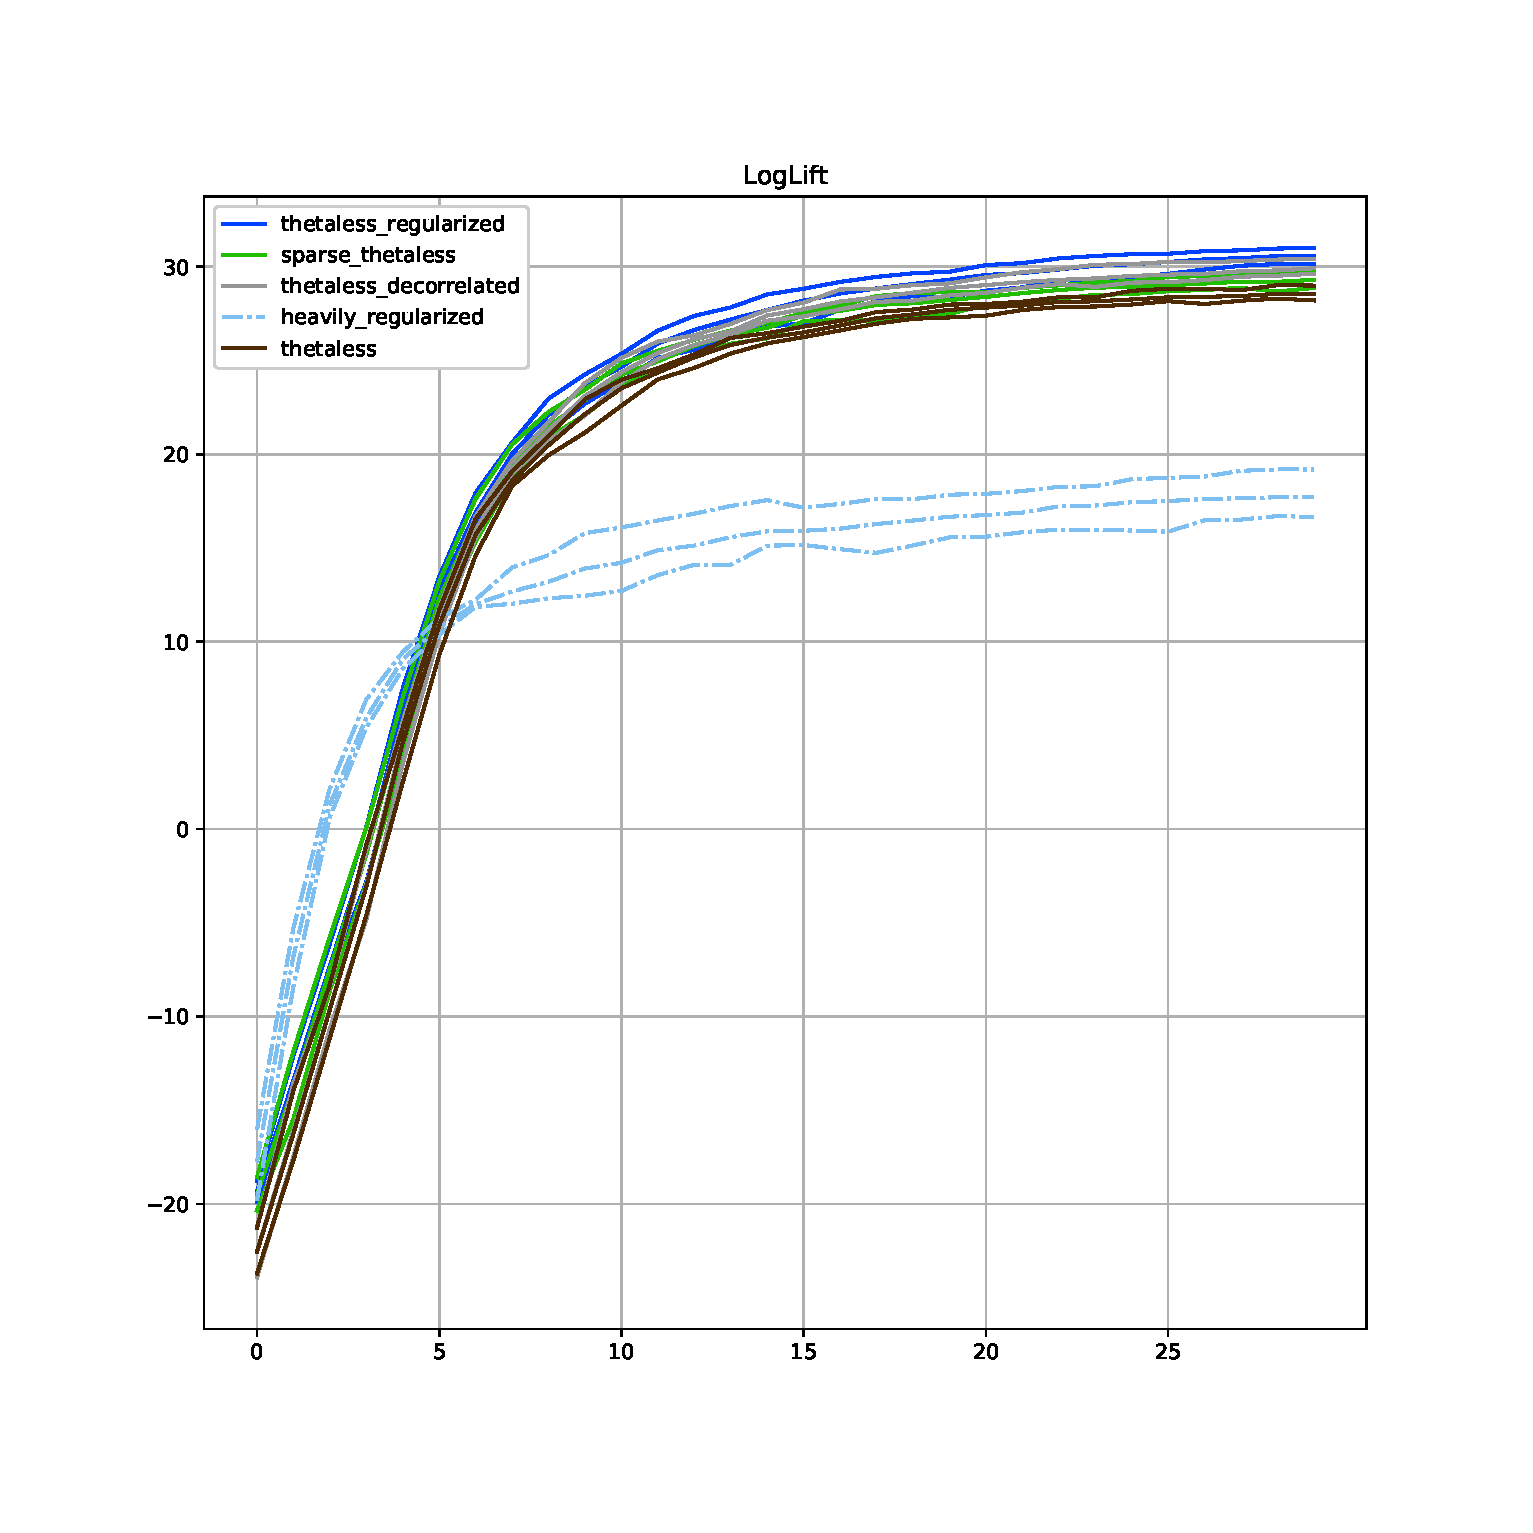
\includegraphics[width=55mm]{images/CH4_improved_loglift30.eps} \\
 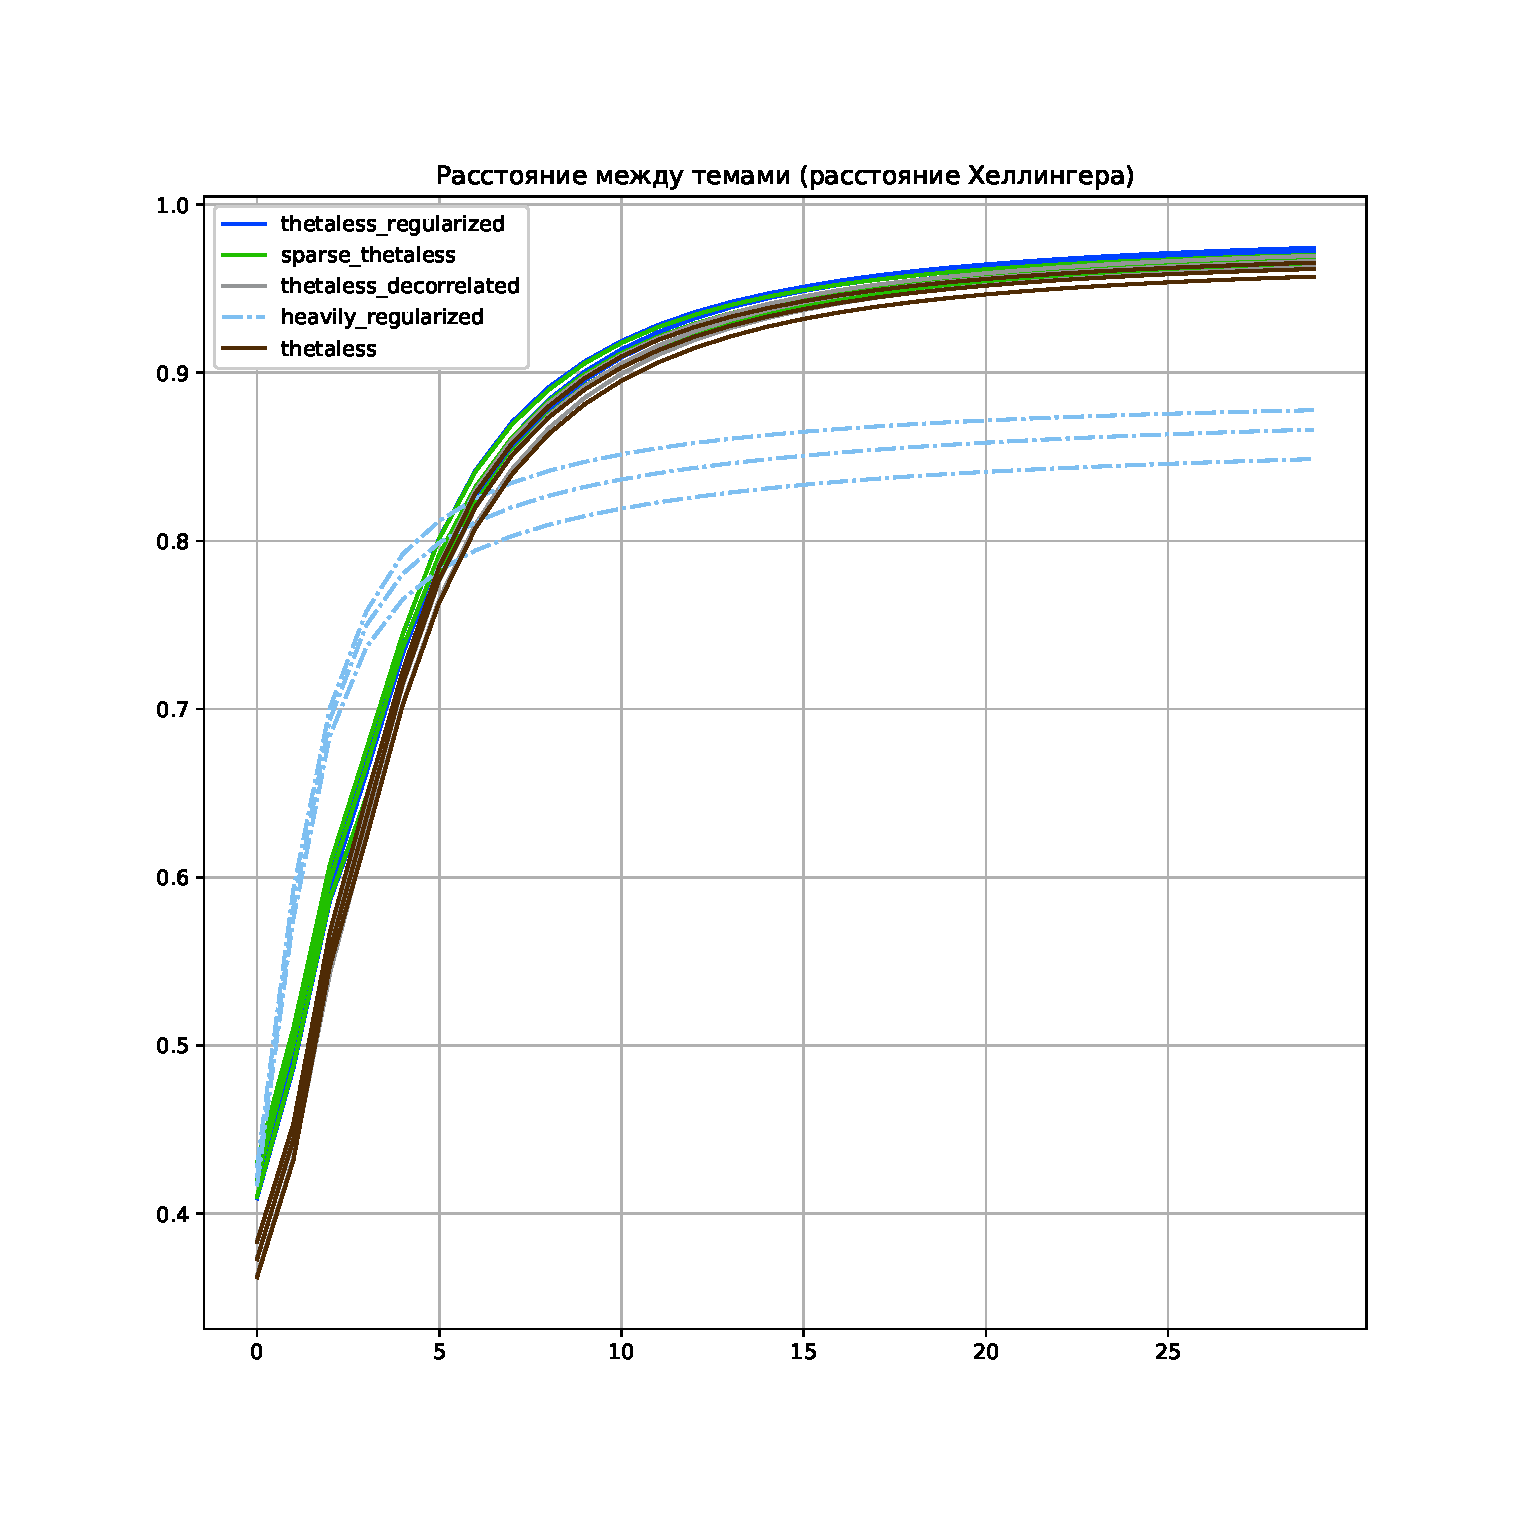
\includegraphics[width=55mm]{images/CH4_improved_diversity_hellinger_False.eps} &   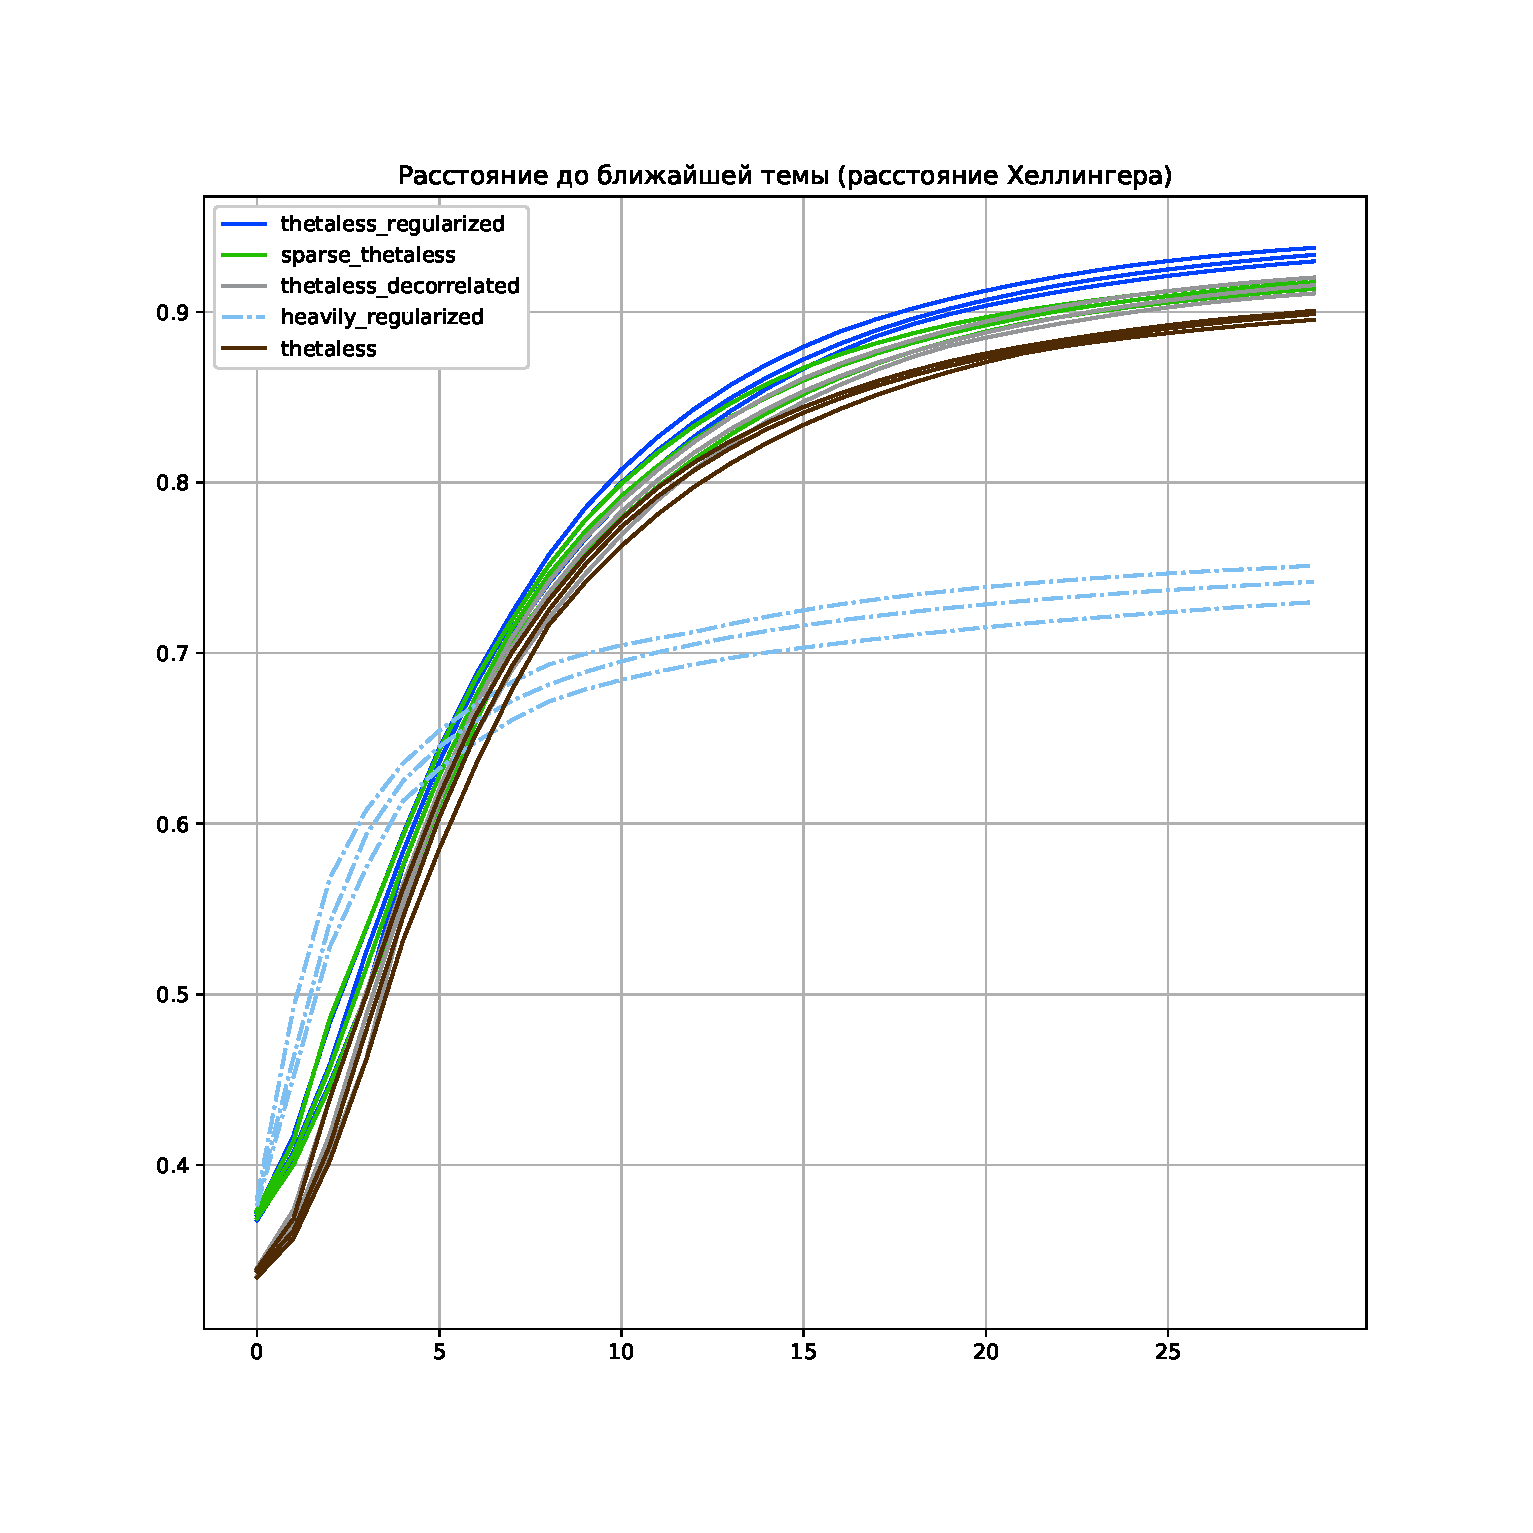
\includegraphics[width=55mm]{images/CH4_improved_diversity_hellinger_True.eps} & 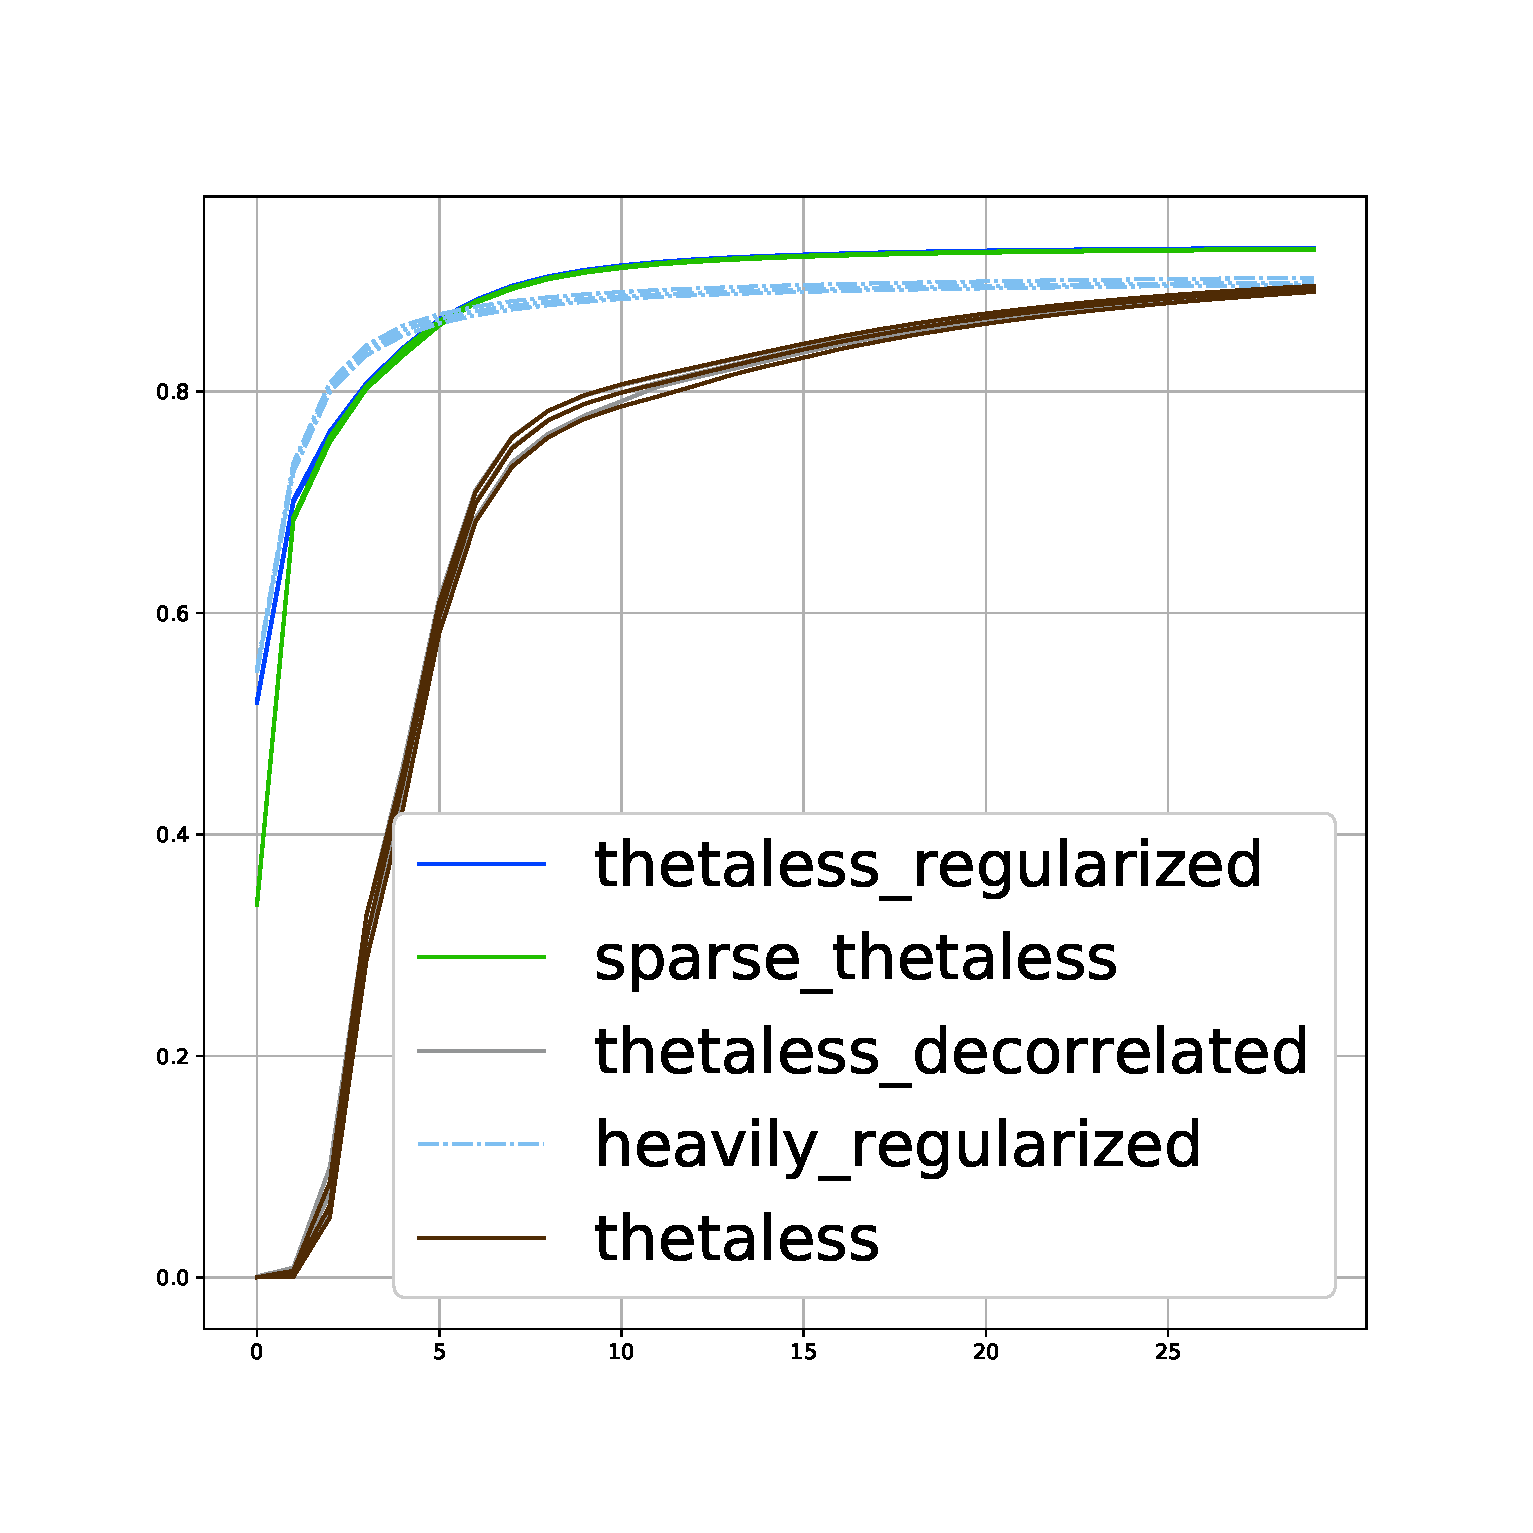
\includegraphics[width=55mm]{images/CH4_improved_SparsityPhiScore.eps} \\    
    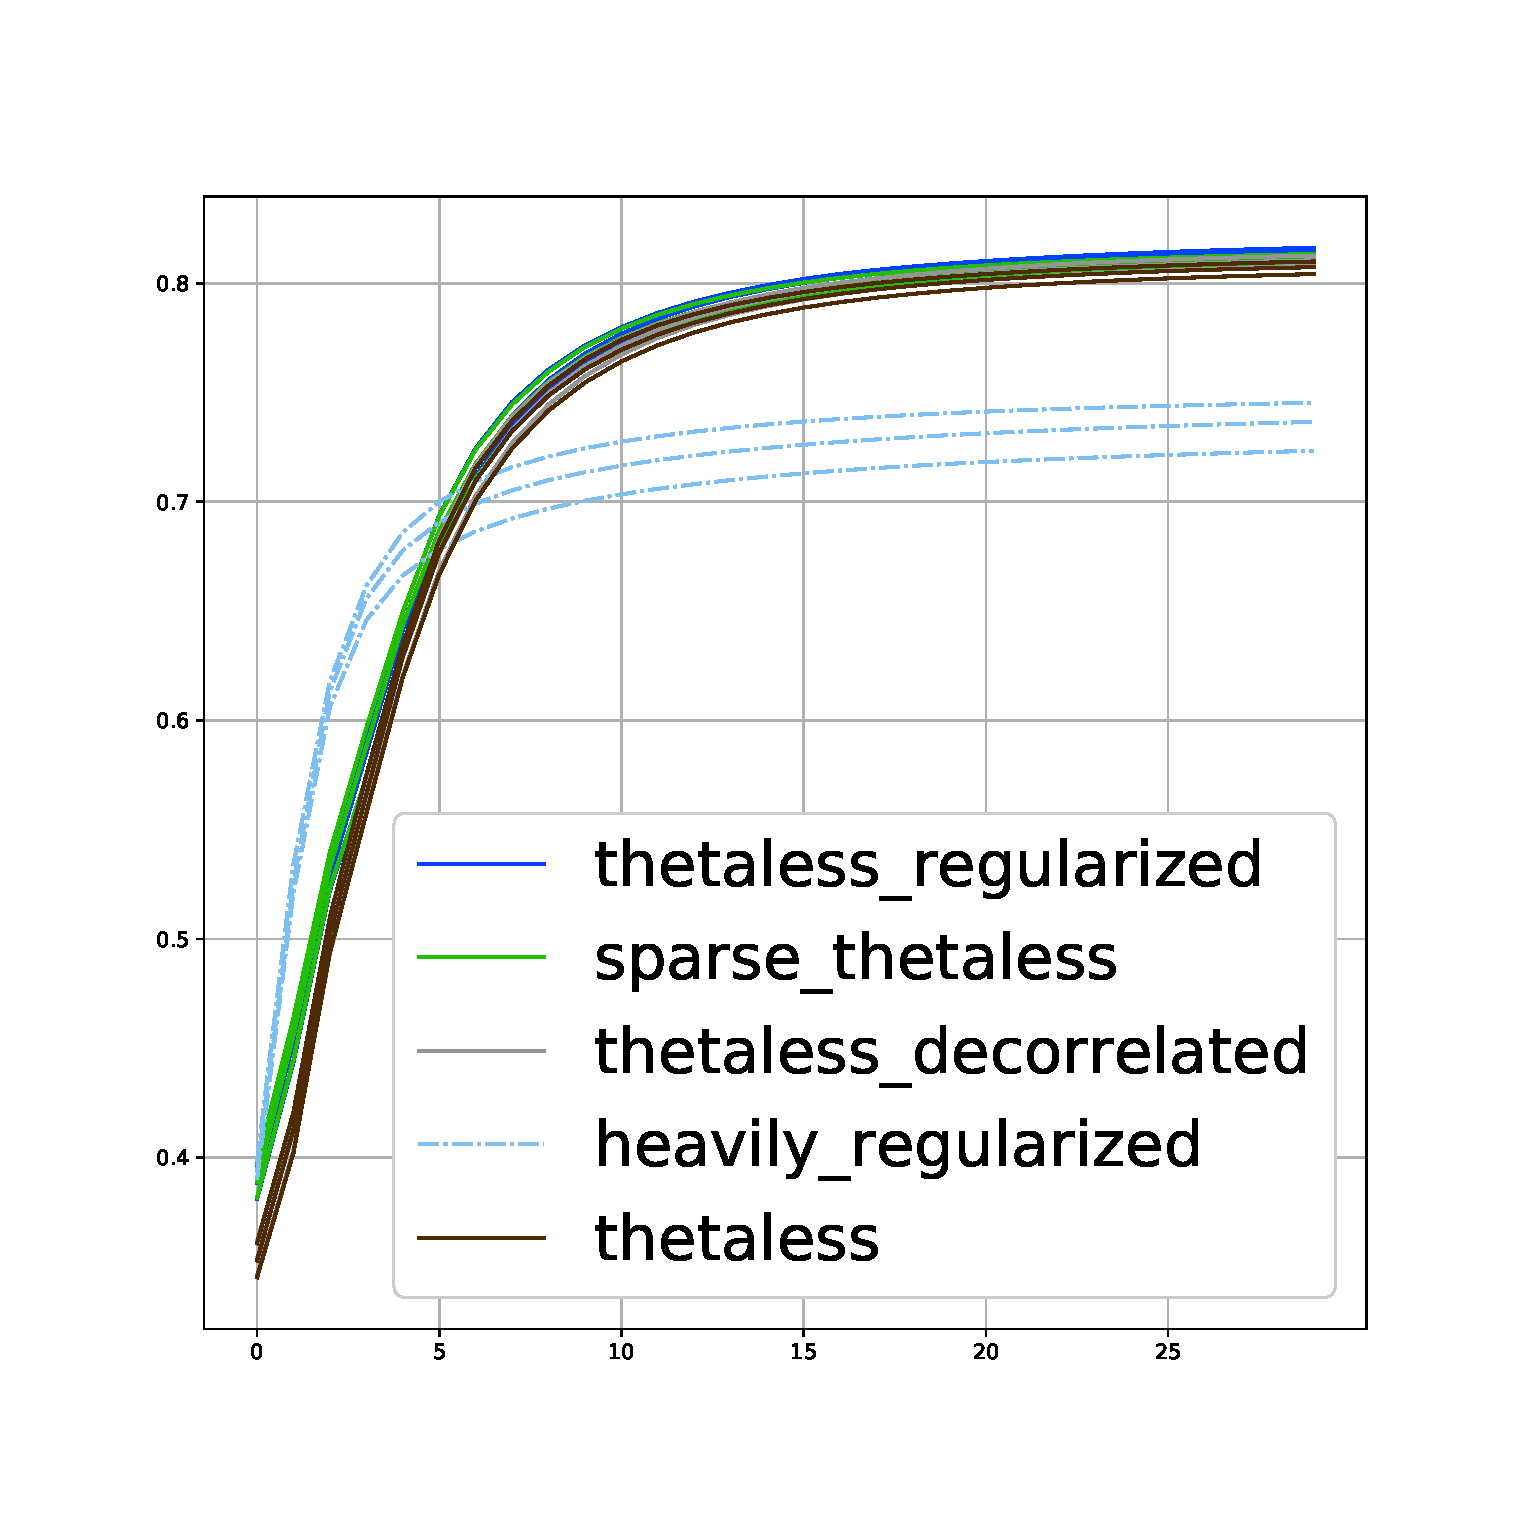
\includegraphics[width=55mm]{images/CH4_improved_diversity_jensenshannon_False.eps} &   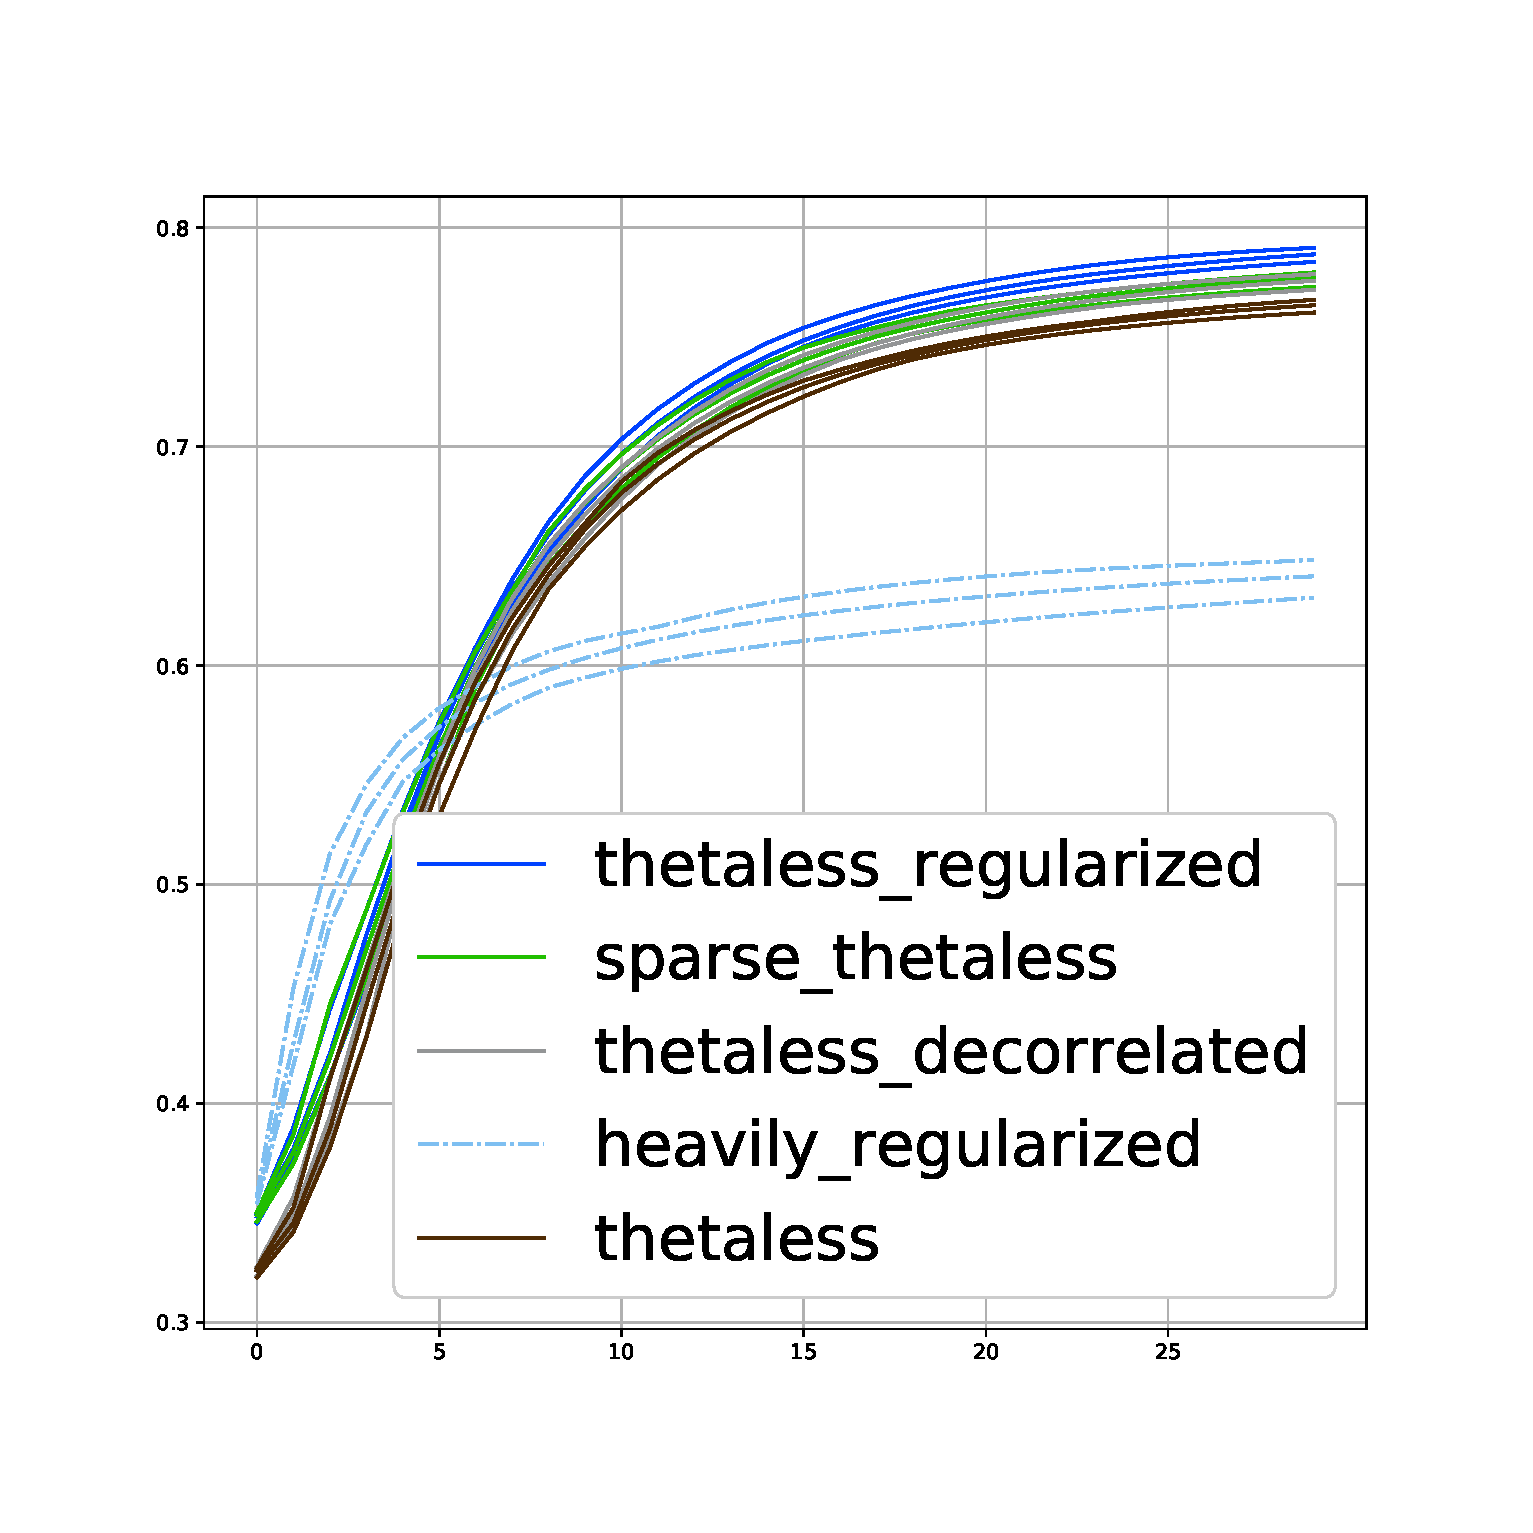
\includegraphics[width=55mm]{images/CH4_improved_diversity_jensenshannon_True.eps} & 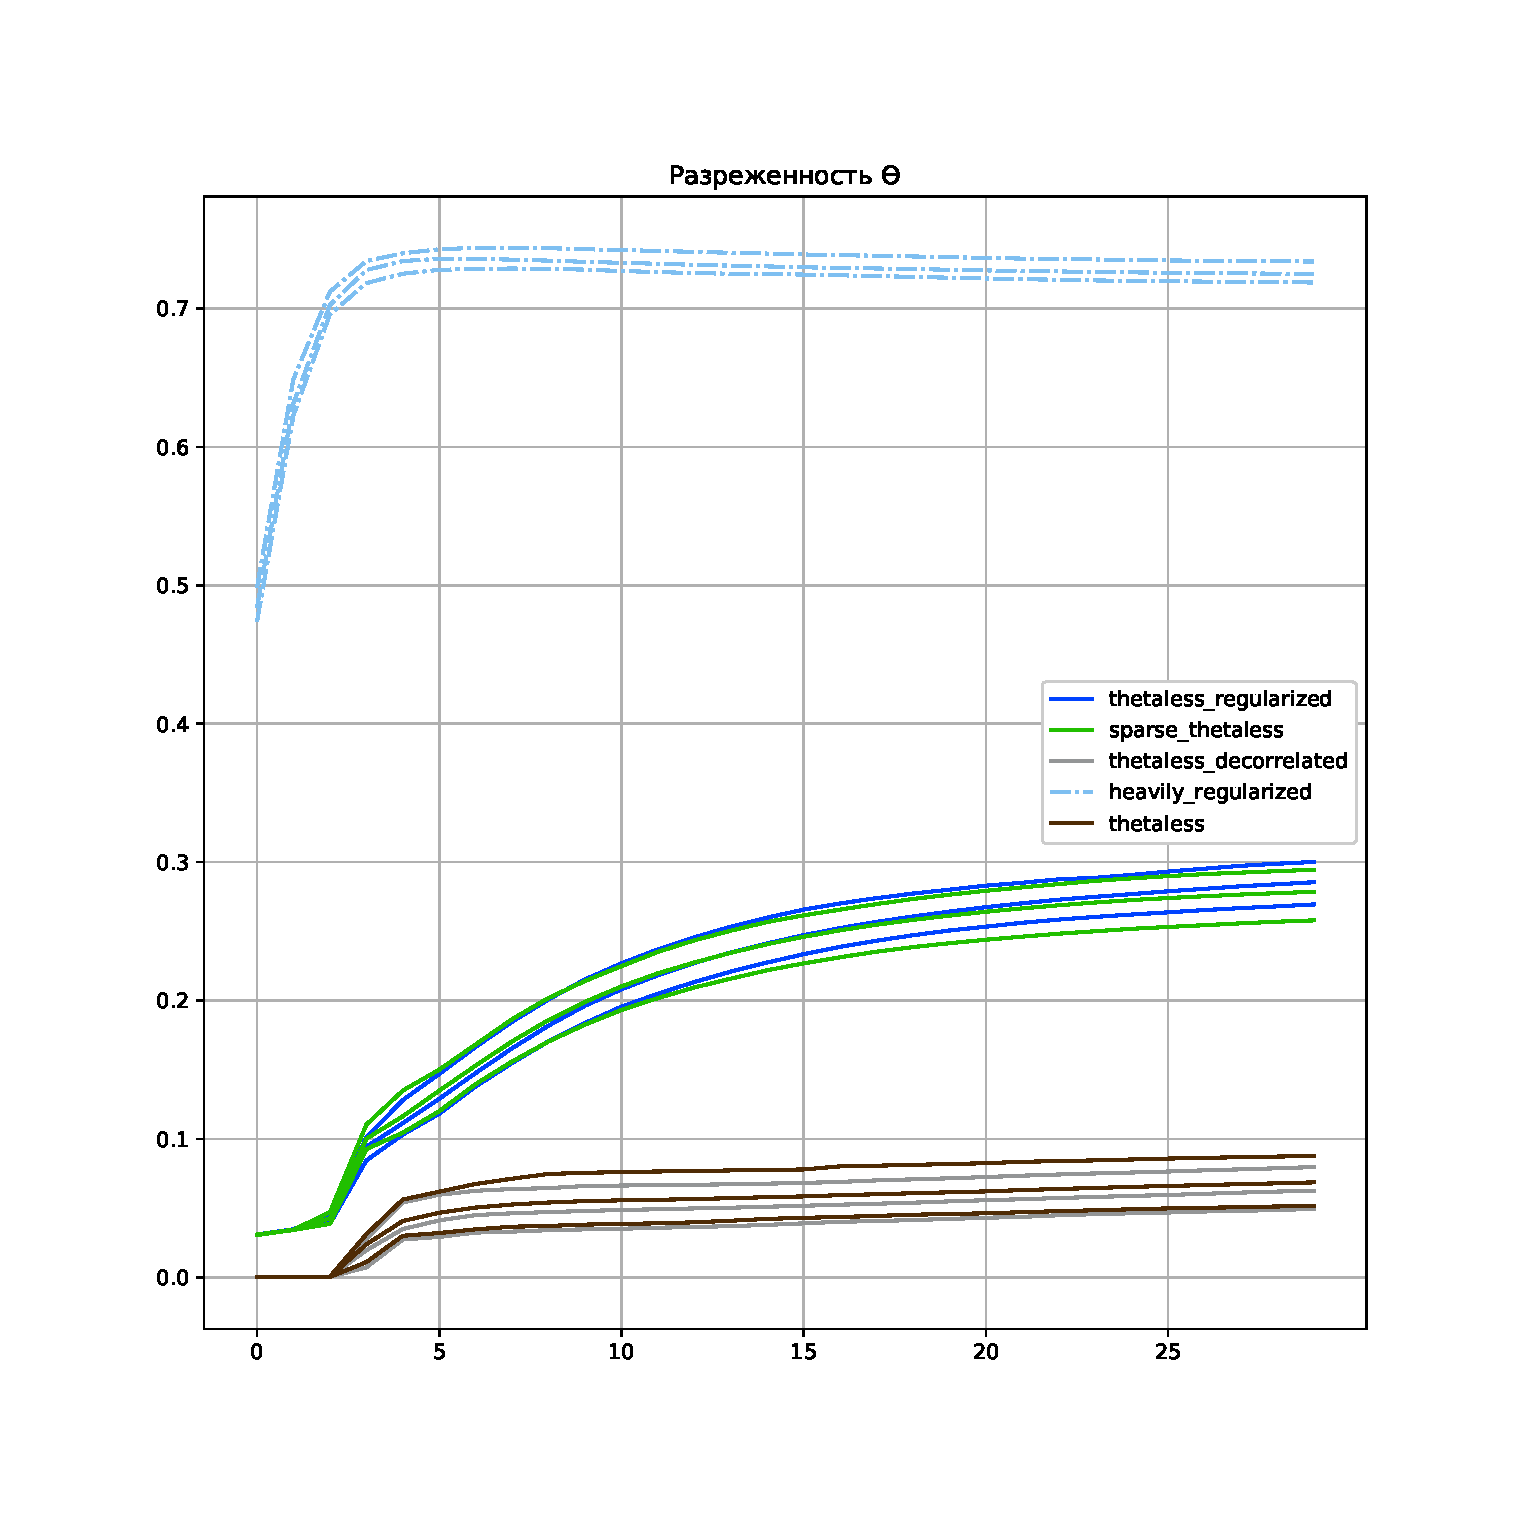
\includegraphics[width=55mm]{images/CH4_improved_SparsityThetaScore.eps} \\
\end{tabular}
    \caption{Графики зависимости различных критериев качества тематических моделей для пяти моделей (TARTM, PLSA, LDA с 3 видами приоров). Каждой модели соответствуют три линии: среднее значение, минимум и максимум (по пяти случайным перезапускам).}
\label{fig:ch4_improved}
\end{figure}


\begin{figure}
\begin{tabular}{ccc}
    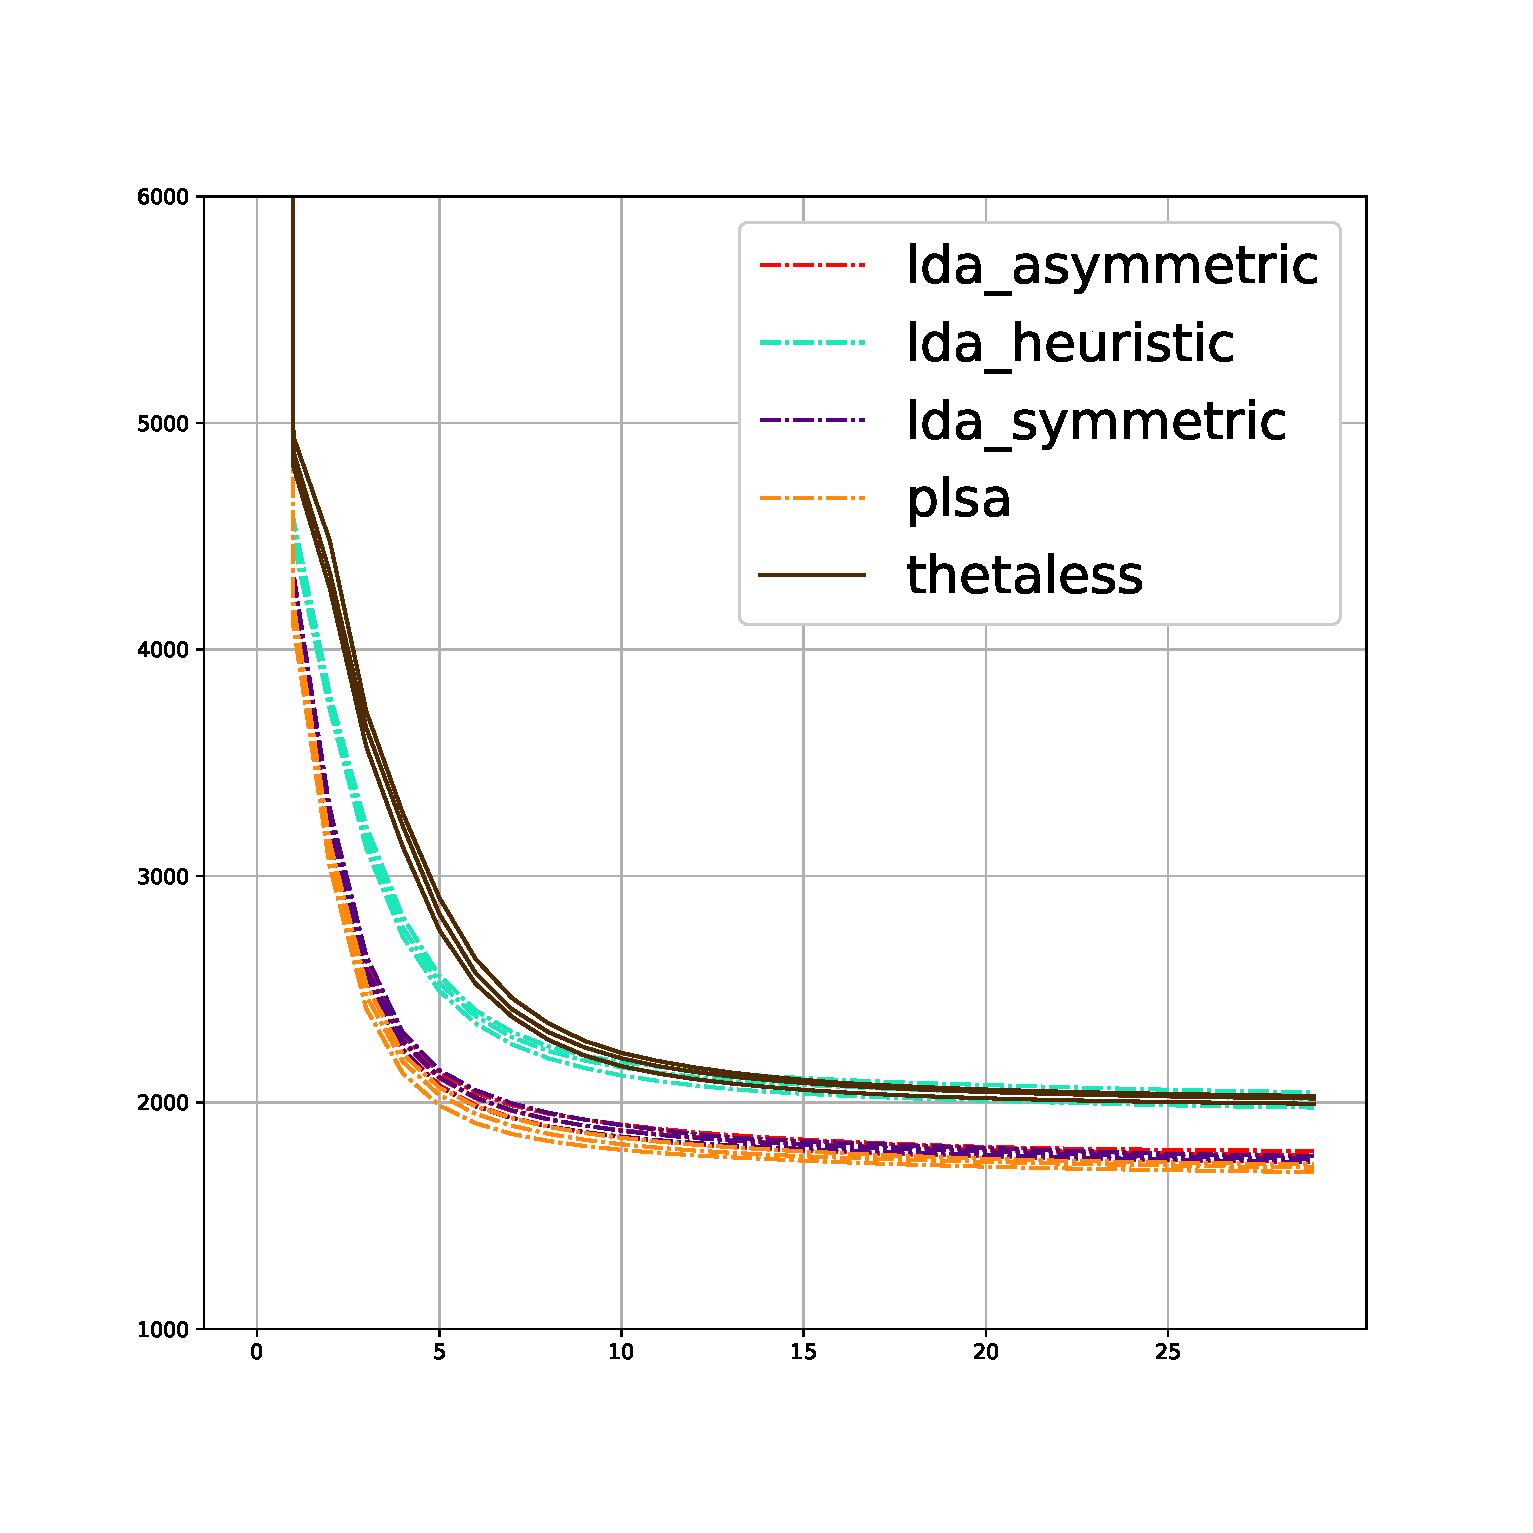
\includegraphics[width=55mm]{images/CH4_baselines_PerplexityScore.eps} &   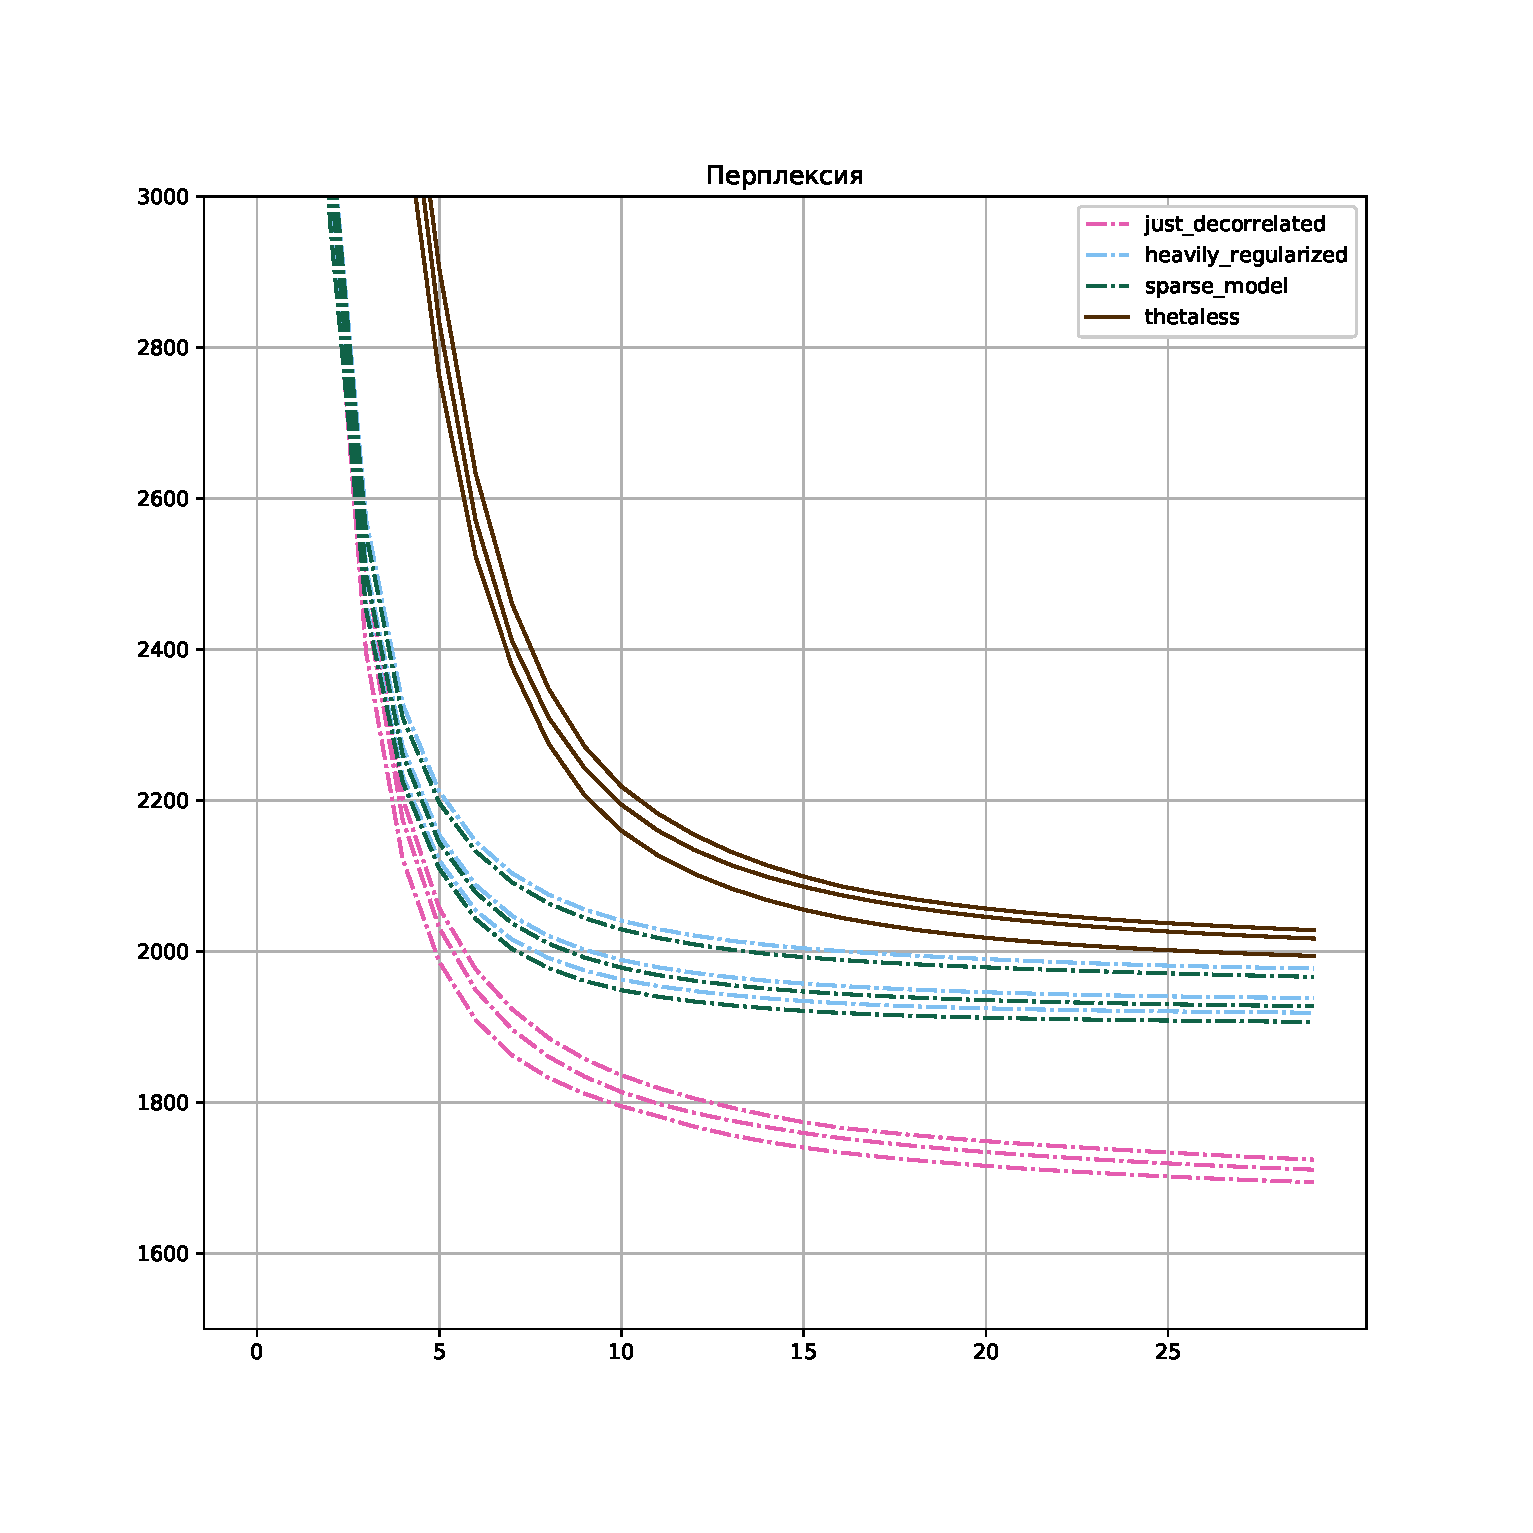
\includegraphics[width=55mm]{images/CH4_vs_regularized_PerplexityScore.eps} & 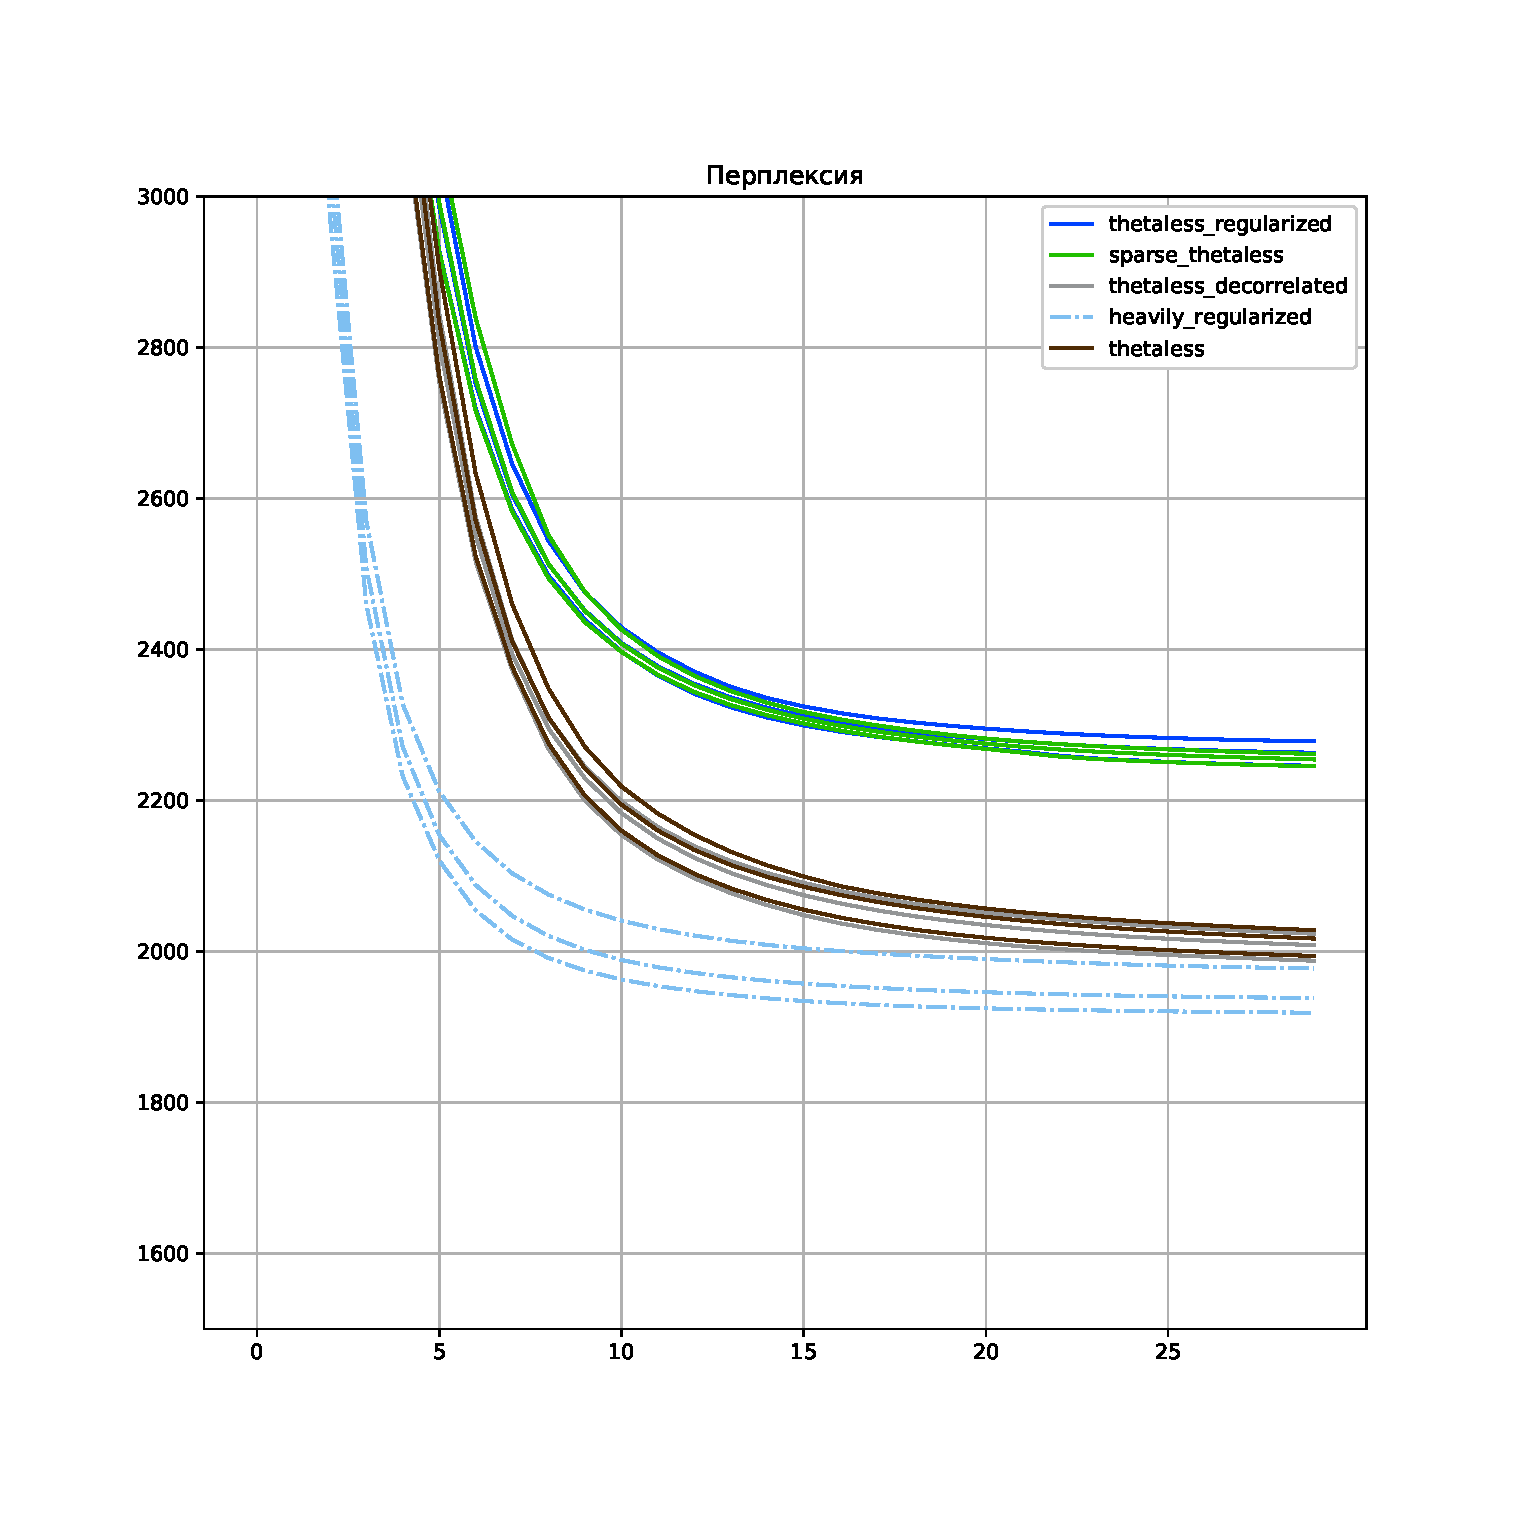
\includegraphics[width=55mm]{images/CH4_improved_PerplexityScore.eps} \\
    (a) first & (b) second & (c) third \\[6pt]
\end{tabular}
\label{fig:Perple3x}
\end{figure}



\textbf{Сравнение с PLSA/LDA}. На рисунке \ref{fig:ch4_base} видно, что предлагаемый псевдорегуляризатор позволяет строить модели, темы которых более уникальны, чем темы классических моделей (среднее расстояние между темами и среднее расстояние до ближайшей темы у TARTM больше, чем у других моделей; коэффициент подобия Жаккара, напротив, меньше). Также можно заметить, что введение певдорегуляризатора не слишком негативно сказалось на перплексии (конечная перплексия сравнима с перплексией \texttt{lda\_heuristic}). Мера качества LogLift показывает улучшение более чем в два раза.

Предлагаемая модель уступает лишь в разреженности матрицы $\Theta$, что вполне ожидаемо (в самом деле, матрица $\Theta$ уже не оптимизируется моделью в явном виде). Заметим при этом что она показывает наилучший результат по разреженности матрицы $\Phi$.

\textbf{Сравнение с регуляризованными моделями}. Рисунок \ref{fig:ch4_vs_reg} демонстрирует схожую картину: рассматриваемый псевдорегуляризатор превосходит остальные модели по LogLift и по критериям качества, связанным с различностью тем.

Две модели, в которых явно введён регуляризатор разреживания, показывают наилучший результат по разреженности матриц $\Theta$ и $\Phi$. Тем не менее, TARTM имеет сравнимую разреженность матрицы $\Phi$ (но этот результат достигается за большее число итераций). 

\textbf{Взаимодействие с дополнительными регуляризаторами}. Рисунок \ref{fig:ch4_improved} показывает, что формула \ref{eq:Mstep_noTheta} успешно комбинируется с другими регуляризаторами ARTM, за счёт чего можно улучшить критерии качества ещё больше. TARTM с традиционным набором регуляризаторов (сглаживание фоновых тем, разреживание предметных тем, декорреляция) выигрывает у аналогичного ARTM по разреженности.

% Это говорит о том, что описанная здесь комбинация осмысленна.
% и проверить взаимодействие предложенной формулы с дополнительными регуляризаторами.
% что позволяет дополнительно .

\textbf{Сравнение по когерентности}. У построенных моделей была несколькими способами измерена когерентность. 

Поточечная взаимная информация (Pointwise Mutual Information, PMI) и положительная поточечная взаимная информация (Positive Pointwise Mutual Information, PPMI) расчитывались как $\log\frac{|D| N(w,v)}{N(w)N(v)}$. В этой формуле участвует $N(w,v)$~--- число документов, в~которых встречаются оба слова $w$~и~$v$,
$N(w)$~--- число документов, содержащих слово~$w$ ($N(w,v)$ и $N(w)$ замерены по той же коллекции что и обучалась модель). Разница между PMI и PPMI состоит в том, что для последнего отрицательные значения логарифма заменяются на нули. Когерентность модели определяется как средние $\mathrm{PMI}(w,v)$ и $\mathrm{PPMI}(w,v)$ по~всем темам и всем парам верхних слов в~каждой теме.

Для подсчёта UMass-когерентности использовался онлайн-сервис Palmetto. Palmetto позволяет оценивать когерентность множества слов при помощи статистики совстречаемости, собранной на английской Википедии. Когерентность множеств из 10 верхних слов каждой темы измерялась по отдельности. На основе полученной выборки из 20 (или 21) чисел были рассчитаны среднее, медиана, стандартное отклонение.

Приведённые в таблице \ref{tab:theta_coh} результаты (все приведённые числа --- усреднения по пяти перезапускам) показывают, что TARTM превосходит остальные модели в терминах документной совстречаемости верхних слов; дополнительная регуляризация незначительно улучшает это далее. Отдельно стоит обсудить значения UMass-когерентности: как видно из сравнения среднего, медианы и стандартного отклонения, регуляризация ухудшает ``среднее'' качество тем, но усиливает разрыв между хорошими и плохими темами. Это можно объяснить тем, что TARTM имеет тенденцию выделять частые, но неинформативные слова в отдельную тему; Рис \ref{fig:2topics} демонстрирует это на примере двух сравнимых тем.

\begin{figure}
\begin{tabular}{lrrrrr}
\toprule
{} &  umass &   pmi &  ppmi &  median\_umass &  std\_umass \\
model\_type            &        &       &       &               &            \\
\midrule
heavily\_regularized   & -2.121 & 1.625 & 1.710 &        -1.964 &      1.021 \\
plsa                  & -1.850 & 1.483 & 1.517 &        -1.826 &      0.671 \\
thetaless             & -1.914 & 1.694 & 1.716 &        -1.709 &      0.831 \\
thetaless\_regularized & -2.195 & 1.729 & 1.788 &        -1.826 &      1.220 \\
\bottomrule
\end{tabular}
    \label{tab:theta_coh}
\end{figure}

\begin{table}[t]
    \caption{Примеры верхних слов в двух сравнимых темах.
        Слова общей лексики выделены жирным шрифтом.
        TARTM выделяет слова общей лексики в~отдельные темы, в~отличие от модели~PLSA.}
    \label{fig:2topics}
    \small
    \begin{tabular}{ | p{7.5cm}| p{7.5cm} |}
    \hline
    TARTM &  PLSA
    \\ \hline	
game play team win player hit season lose fan league & \textbf{year} game \textbf{last} win play lose team hit player \textbf{guy}
    \\ \hline
\textbf{make} \textbf{point} \textbf{even} \textbf{case} \textbf{mean} \textbf{keep} \textbf{long} \textbf{actually} \textbf{consider} \textbf{every} & \textbf{make} \textbf{even} \textbf{may}  \textbf{case}  \textbf{consider}  fire  \textbf{less}  \textbf{mean}  \textbf{long}  force
    \\ \hline
    \end{tabular}
\end{table}

\subsection{Интуитивное объяснение особенностей TARTM}

Основное объяснение полученных результатов следующее. PLSA и LDA предсказывают появление слов в документах как с помощью матрицы $\Phi$, так и с помощью матрицы $\Theta$, в то время как TARTM использует только матрицу $\Phi$. Это означает, что PLSA и LDA могут ``скорректировать'' недостатки матрицы $\Phi$ за счёт правильного подбора матрицы $\Theta$, а TARTM может ``исправлять'' эти недостаки только меняя саму $\Phi$.

Приведём простой пример, иллюстрирующий данные рассуждения. Допустим, коллекция состоит из 4 слов и 3 документов: \texttt{herbs and spices}, \texttt{spices and medicine}, \texttt{herbs and medicine}. Таким образом, матрица $n_{dw}$ равна

\begin{center}
\begin{tabular}{l|llll}
$n_{dw}$   & and & herbs & spices & medicine \\ \hline
doc1       & 1   & 1     & 1      & 0        \\
doc2       & 1   & 0     & 1      & 1        \\
doc3       & 1   & 1     & 0      & 1       
\end{tabular}
\end{center}

Предположим, что мы хотим построить тематическую модель с четырьмя темами. Тематическая модель, наиболее простая из всех возможных, выделяет каждое слово в отдельную тему (иными словами, $\Phi = I$, а $\Theta = \frac{1}{3} n_{dw}$):
\begin{minipage}[t]{0.25\textwidth}
\[
\Phi_{tw} = 
\begin{pmatrix}
    1 & 0 & 0 & 0 \\
    0 & 1 & 0 & 0 \\
    0 & 0 & 1 & 0 \\
    0 & 0 & 0 & 1 \\
\end{pmatrix},
\]
\end{minipage}\begin{minipage}[t]{0.2\textwidth}
\[
\Theta_{td} = \frac{1}{3} 
\begin{pmatrix}
    1 & 1 & 1 & 0 \\
    1 & 0 & 1 & 1 \\
    1 & 1 & 0 & 1 \\
\end{pmatrix}.
\]
\end{minipage}

Проведённый численный эксперимент показал, что TARTM успешно восстанавливает описанное выше решение в 998 из 1000 случаев. Тем не менее, это решение не является единственным. Большинство найденных при помощи PLSA тематических моделей содержат коэффициенты, не кратные $\frac1{3}$. Ни один из 1000 случайных перезапусков PLSA не дал описанную выше естественную тематическую модель. В качестве примера приведём такую модель:
\[
\Phi_{tw} = 
\begin{pmatrix}
    0.044 & 0.956 & 0 & 0 \\
    0.488 & 0 &  0 & 0.512 \\
    0.488 & 0 & 0.512 & 0 \\
    0.281 & 0 & 0.279 & 0.44 \\
\end{pmatrix},
\]
\[
\Theta_{td} = 
\begin{pmatrix}
    0.349 & 0 & 0.651 & 0 \\
    0 & 0.008 & 0.244 & 0.748 \\
    0.348 & 0.652 & 0 & 0 \\
\end{pmatrix}.
\]
Несмотря на то, что матрица $\Phi$ не разделяет искомые ``идеальные'' темы и является зашумлённой, комбинация $\Phi$ и $\Theta$ адекватно описывает $n_{dw}$ (нетрудно убедиться, что $\Phi \cdot \Theta \approx \frac{1}{3} n_{dw}$).\\

Недостатком этого примера является его искусственность: поскольку $|W|=|T|$, $|T|>|D|$, то задача матричного разложения допускает точное (а не приближённое) решение. Можно привести и более правдоподобный пример, демонстрирующий то же явление. Рассмотрим следующую коллекцию из 7 слов и 6 документов:
\begin{verbatim}
medicine and spices
herbs and spices
herbs and spices and chicken
honey and spices
medicine and herbs
medicine and honey 
\end{verbatim}

Как могла бы выглядеть ``хорошая'' тематическая модель из 4 тем, построенная на этой коллекции? Неинформативное слово \texttt{"and"} может либо лежать в какой-то единственной ``фоновой'' теме ($\exists t_0: \phi_{wt_0} > 0, \phi_{w\ast} = 0$ для $w=$\texttt{"and"}), либо распределиться между несколькими ``информативными'' темами. Первый вариант кажется более естественным. Из 1000 запусков PLSA и TARTM с разными начальными приближениями PLSA ни разу не выделил \texttt{"and"} в отдельную тему, в то время как TARTM сделал это в 365 случаях. При этом матрица $\Theta$, полученная в TARTM содержала от 3 до 7 нулей, а в PLSA от 12 до 17. Это показывает как PLSA с помощью нулей в матрице $\Theta$ ``прячет'' недостатки, вызванные шумами в виде наличия \texttt{"and"} во всех темах.

\section{Заключение}

В данной работе была предложена модификация оптимизационной задачи в тематическом моделировании, которая уменьшает количество оптимизируемых параметров и повышает уникальность и когерентность получаемых тем. Предложенный алгоритм не увеличивает вычислительную сложность или количество необходимых обучающих примеров. Эксперименты на реальных данных показывают, что предложенный алгоритм действительно улучшает качество тем.

Важным аспектом предлагаемого алгоритма является его совместимость с подходом ARTM, что позволяет включать произвольное количество дополнительных регуляризаторов, чтобы точно настроить решение поставленной задачи.